% test comment
\documentclass[12pt,letterpaper]{report}

\usepackage[utf8]{inputenc}
\usepackage{preamble}	%a local package of packages used in this document
	% All packages from this preamble were moved to the main file. 




\title{
	{\textbf{Orientation-dependent Surface Energy Characterization of Rare-Earth-Free Magnetostrictive Alloys for Abnormal Grain Growth Modeling }}\\
	{\large University of Maryland, College Park}\\
}
\author{\makebox[.9\textwidth]{\textbf{Michael N. Van Order}\thanks{Funded by the \NSF SUSCHEM - Collaborative Research program (grant number: DMR-1310447)}}\\~\\
	%		Materials Science and Engineering\\
	%		University of Maryland
	\and Dr. Alison Flatau\\
	%		Aerospace Engineering\\
	%		Univeristy of Maryland
	\and Dr. Suok-Min Na\\
	%		Aerospace Engineering\\
	%		University of Maryland
}
\date{20 February 2017}

\doublespacing

\begin{document}	


\chapter*{Abstract}
Abstract goes here. Yeah. You will do this last. 

High sensitivity semiconductor, optical, and sensing devices require single crystal metals for their isotropy which allows for unique material properties. However they are expensive and difficult to produce. By using abnormal grain growth (AGG) techniques, our group can produce single-crystal-like materials that achieve ~90\% performance of true single-crystals at ~5\% of the cost. Fully understanding AGG mechanisms is crucial to the growth of high quality, cost effective alloy fabrication. Many advances have been made to understand key parameters of AGG, and we postulate that the final piece lies in understanding the surface energy of our alloys. While several surface energy measurement techniques have been developed for low-energy plastic surfaces, high-energy metal surfaces have largely been ignored due to the complexity of sample preparation and experimentation. This dissertation investigates three measurement techniques targeted for high-surface-energy iron-alloy crystal facets. \par
The first of these techniques, the gallium drop contact angle method, examined a droplet of liquid metal gallium resting on our metal sample. By recording shape of this droplet, a value for surface energy of targeted crystal orientations is acquired using our derived thermodynamically-based mathematical model. This study experimentally confirmed trends that are predicted in theoretical models, but identified that oxide formation on the sample surface interferes with acquisition of accurate quantitative results. This revelation led to a more robust study that expands on classic drop shape analysis techniques and eliminates complications associated with oxide layer formation. I performed and analyzed multiple oxide removal procedures using X-ray photoelectron spectroscopy. The most promising procedures are polishing in an inert atmosphere and ion bombardment cleaning. Immersing the sample in an oil environment isolates this unstable iron-alloy surface from air and prevents oxidation. While in this environment, samples are probed with a deionized water droplet and a shape analysis is performed to calculate surface energy values using the Schultz method. I modified this method by utilizing a technique previous only used on plastics to prevent water from spreading. I hypothesize that patterning sample surfaces with an ion mill will stabilize droplets during shape measurements, thus generating reliable surface energy calculations. Success of this experiment could allow metallurgists to finally experimentally measure surface energy for any metal surface, thus providing confirmations of theory and sparking new ideas of how grain growth in metals can be controlled and even manipulated. \par 
A study suggested by my committee to expand the scope of my dissertation utilizes the micro-features of my patterned samples from the previous experiment growing equilibrium crystals at high temperatures. This seldom observed phenomenon can identify the temperatures at which specific metal crystals will grow and allow for a fundamental surface energy characterization. This complex and readily available technique will provide completeness to my dissertation and provide a basis for future researchers. This study will ultimately bolster my dissertation for the betterment of the surface science community as well as my own group’s goals of perfecting AGG. 



\begin{titlepage}
	\clearpage 
	\maketitle
	
	\thispagestyle{empty}
\end{titlepage}

\chapter*{Copyright Statement}
I declare that...

\chapter*{Dedication}
To mom, dad, sister, Alyson, and cats.



\chapter*{Acknowledgments}
I want to thank...mom, dad, sister, Alyson. 

Also to James Willems, Elyse Willems, Bruce Greene, Lawrence Sonntag, Adam Kovic, and Matt Peake, in no particular order, from Funhaus, for encouraging this stranger on the internet to do his best and be diligent with his work. Your work ethic is truly something I try to emulate everyday. 

\tableofcontents
\listoffigures
\listoftables

\chapter{Introduction}\label{chapter1}
\section{Background}\label{section1}
%\subsection{Magnetostriction} %without * gives numbered section

\begin{outline}[enumerate]
\1 Magnetostriction
	\2 History and Discovery
		\3 Joule effect
		\3 Villari Effect
	\2 Materials
		\3 Terfenol-D
		\3 Galfenol
		\3 Alfenol
	\2 Uses and Applications
		\3 Sensors
			\4 Whiskers
			\4 Non-contact torque sensors
\1 Galfenol
	\2 Manufacturing 
		\3 Single crystal 
			\4 Arc melting
			\4 Directional solidification
		\3 Polycrystalline rolled thin sheets
			\4 Rolling (hot, warm, cold)
			\4 Atmospheric annealing 
				 Argon\\
				 Sulfur\\
			\4 Benefits
				 Rolling is much cheaper\\
				 Can grow grains to 90\% of sample surface
			\4 Restrictions
\1 Abnormal Grain Growth (AGG)
	\2 Theory
	\2 Proposed Mechanisms
	\2 Latest Research for AGG in Fe-based alloys
	\2 Need for Orientation-dependent Surface Analysis/Surface Energy Measurements
		\3 Latest Research on FeGa Surface Energy 
\1 Surface Energy
	\2 Surface Energy vs. Surface Tension
		\3 solids vs. liquids
		\3 no real difference, same unites but different nomenclature
\1 Methods of Surface Energy Measurement Techniques
	\2 Contact Angles
		\3 Low Energy Surfaces
			\4 Owens-Wendt Method
		\3 High Energy Surfaces
			\4 Cleavage energy\cite{Gilman1960}
			\4 Atomic force curve measurement\cite{Drelich2004}
			\4 Schultz method\cite{Schultz1977,Schultz1977a,Schultz1992}
		\3 
\end{outline}

%\subsection{Physics of Magnetostriction}
%

This section will talk about Magnetostriction and the physics involved in it. 

Unpaired electrons in the valence shell, or unbalanced spins, can produce significant magnetism in an atom.  However, these electrons are used in bonding when forming a solid making their contribution to magnetism in a solid is negligible\cite{Breu2008}.  The preserved magnetic moments in solids are more characteristic of an element’s ionic electron configuration (Fe{$^{3+}$} rather than Fe) or with sufficient bonding electrons added to complete the shell.  The only groups of elements in the periodic table which exhibit magnetic moments in solids are those in which the unbalanced electron populations occur in an inner shell, namely the transition metals (3\textit{d}, 4\textit{d}, and 5\textit{d}), rare earths (4\textit{f}), and actinides (5\textit{f}).  It is clear that the more tightly bound an unfilled orbital shell is, the less the unpaired electrons will have to do with bonding and the more they will contribute to magnetism.  This is why we see very strong magnetic responses in rare earth materials which use 6\textit{s} and 5\textit{d} shells for bonding before using the very tightly bound 4\textit{f} shell electrons.  The 3\textit{d} electrons in transition metals are less tightly bound to the nucleus, and sometimes 3\textit{d} electrons are used for bonding.  \\

\begin{figure}[h] 
	\centering
	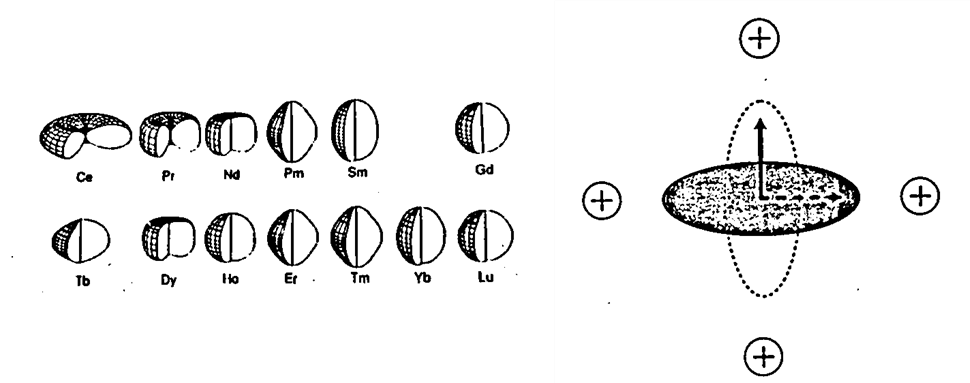
\includegraphics[trim=0pt 10pt 0pt 0pt,scale=1.0]{electron_cloud_density}
	\caption{(a) 4f electron charge cloud densities for a number of rare earth elements. (b) Schematic of oblate 4f charge density of a rare earth element with + nearest neighbors, such as Tb, rotating in a magnetic field. \cite{Engdahl1999} 
	}
	\label{fig:electron_cloud_density}		
\end{figure}

Magneto-elasticity is the coupling between a material’s classical properties of elasticity and strain and the quantum mechanical and relativistic phenomena of magnetism.  When a spin imbalance occurs, electrons can order in such a way that the net magnetic moment points in a particular direction which lowers the crystal symmetry and produces new properties, like magnetostriction.\cite{Breu2008} This coupling between magnetism and elasticity derives from the large contribution of the spin moment to the magnetic moment.  Hence, coupling occurs if there is a strong coupling between the \textit{direction} of the atom’s spin moment and the \textit{orientation} of its anisotropically shaped electron charge cloud, as seen in Figure 1a.  This coupling that exists at the individual electron level is called “spin-orbit coupling,” and since it derives from relativistic aspects of the electron motion, it is one of the smallest energies used to describe the state of an atom.  It is easiest to see this coupling in rare earth elements where the spin directions of rapidly moving 4\textit{f} electrons are strongly coupled to the orientation of their orbits.  This individual electron spin-orbit coupling leads to strong coupling between the total spin moment and the total electron density.  Thus, in rare earth elements the spin moment can be envisioned as rigidly attached to the anisotropically shaped electron charge cloud.  We can now define magnetic anisotropy as the tendency of a magnetic moment to point in a specific crystalline direction, the easy magnetization direction, because of the electrical attraction/repulsion between the rotating electronic charge cloud and neighboring charged ions, as seen in Figure 1b.  It is important to note that 3d electrons obey the same magnetoelastic trends, but with a factor of ten less for spin-orbit coupling.\cite{Engdahl1999}

%testasdasdasasdasdas
%test again
%\subsection{Materials for Magnetostriction}\label{magnetostrict-materials}
%
	
This section talks about commercial magnetostrictive materials, what alternatives are available, why we study them, and what we can do with them. 

\begin{figure}[h] 
	\centering
	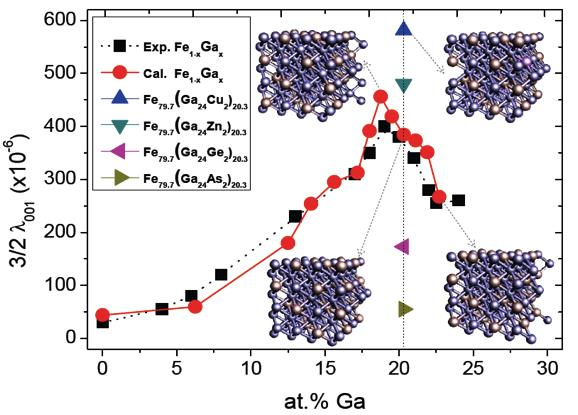
\includegraphics[trim=0pt 10pt 0pt 0pt,scale=1.5]{galfenol-composition-constant}
	\caption{Calculated tetragonal magnetostriction constant (3/2)$\lambda_{001}$ (red circles) and experimental data taken at room temperature (black squares at different Ga concentrations). Triangles show results of four ternary alloys with addition of Cu, Zn, Ge and As. %Insets give the crystal structures with purple and red balls for Fe and Ga atoms, respectively.%
	}
	\label{fig:galfenol-composition-constant}		
\end{figure}

Magnetostriction \cite{Ueno2015a} is the structural response of magnetic materials to an external magnetic field, which arises due to the dependence of the magnetocrystalline anisotropy energy on strain. The magnetostrictive coefficient $\lambda$, which is the ratio of the magnetoelastic coupling b to the shear modulus ($\lambda = b/C'$), serves as a figure of merit for magnetostrictive performance. Magnetostriction in Terfenol-D can be traced back to the strong spin-orbit (magnetoelastic) coupling of the lattice to the anisotropic electron cloud surrounding the Tb ion. The understanding of magnetostriction in Galfenol is more challenging, because spin-orbit coupling is generally weaker in the 3\textit{d} transition metals and the electron cloud surrounding the Fe ion is more deformable than for Tb or other rare-earth ions. Although some extrinsic origins have been proposed, it is believed that the enhanced magnetostrictive response of Galfenol results from intrinsic factors, namely, changes in the electronic structure due to Ga ordering. For Galfenol and  several related alloys with low Ga concentrations ($0\% < x < 14\%$), DFT calculations performed with the correct, experimentally observed ordered structures can satisfactorily reproduce the experimental dependence of $\lambda_{001}$ on alloy composition as shown in Fig. \ref{fig:galfenol-composition-constant}. 

When dealing with real alloys with varying degrees of chemical order, we used ab-initio AIMD for the determination of structures in a reasonably large supercell, and the trend of magnetostriction around $x=19\%$ can also be captured. Similar to the auxetic properties of Galfenol, growth of the magnetostriction can be explained, in part, by growing elastic anisotropy and the softening of the shear modulus, $C'$. However, the evolution of magnetoelastic coupling with composition is equally important. With the complete quantum mechanical information, we traced the origin of largely enhanced magnetostriction to individual atoms and pairs of electronic states. In particular, the local short range ordering such as the formation of B2 and D0$_{3}$ coordinates becomes an extremely important factor in the magnetostriction at high Ga concentrations. We expect that the composition ratios and atomic arrangements in the surface and interface regions differ from that in the bulk and can be modified with the exposure to different gases during high temperature anneal. 

%\subsubsection{Applications in Devices}
%
%\subsubsection{Commercially made by ETREMA}
%%TODO Research currently made products by ETREMA
%Woah Text

\subsection{Devices from Aerosmart Lab}

\subsubsection{Whiskers for bridge scour}

\subsubsection{Energy Harvester}
Energy harvesting from ambient vibrations has the potential to bring battery-free wireless electronics to fruition in the commercial sector. In vehicles, a tire pressure monitoring system equipped with the harvester can be operated without a button cell by using vibrations from the engine as power source. Self-powered autonomous wireless sensor systems can notify factories of structure or machine abnormalities without the need of external power or the hassle of battery replacement. The technology will also be applicable for battery-free remotes used in home automation by pushing a button to send on-off infrared signals, or powering hallway lights from floor vibrations as someone walks. Vibrational energy harvesters can work in conjunction with high capacitance devices, supercapacitors, for energy storage undergoing frequent charge and discharge cycles at high current and short duration, like a portable, self-charging cell phone charger. Technologies that convert vibrational energy into electrical power include piezoelectric materials \cite{Gonzalez2002}, electromagnetic induction\cite{Saha2008}, and magnetostriction\cite{Ueno2011}. 


There are few commercial energy harvesters being used effectively as barriers to widespread implementation exist. Specifically, piezoelectrics are brittle with poor robustness to bending and tension. They also suffer from high output impedance in the M$\Omega$ range, which is a result of their capacitive properties, that transfer only small amounts of electrical energy to external loads. In moving-magnet type harvesters, poor coupling and low resonant frequency up to several Hz results in low output voltage. 
\begin{figure}[h!] %this figure will be at the right with text wrapped around it
	\centering
	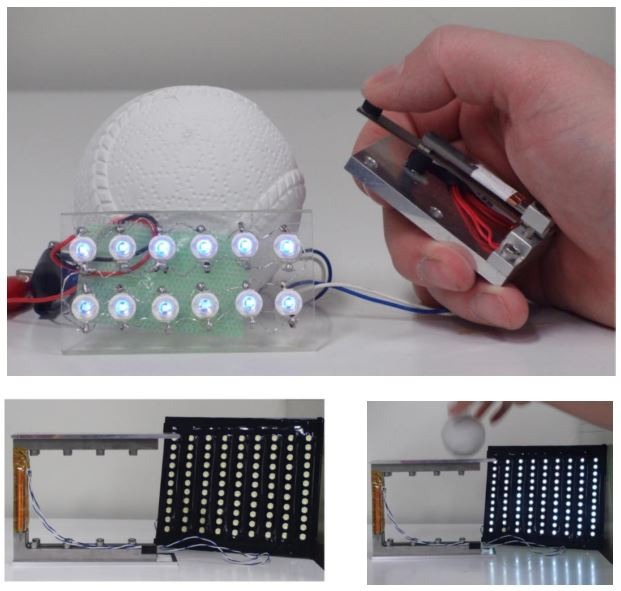
\includegraphics[width=0.5\textwidth]{energy-harvest-demo}
	\caption{Galfenol resonant beam energy harvester. Photo courtesy of Dr. Toshiyuki Ueno, Kanazawa University, Japan. Galfenol beams are in the same region as the coils and have dimensions of 3 mm thick x 15 mm width x 80 mm length.\cite{Slaughter2011}}
	\label{fig:energy-harvest-demo}
\end{figure}
The iron-based magnetostrictive alloy Fe-Ga (Galfenol, \fegacomp) is of interest for actuation, sensing and energy harvesting applications because in addition to its magnetostrictive properties, it is ductile and it has robust mechanical properties\cite{Clark2003}, relatively high permeability and good saturation magnetization (~1.7 T)\cite{Clark2002}. These properties allow our collaborator at Kanazawa University, Toshiyuki Ueno, to prototype highly-scalable Galfenol energy harvester devices with high efficiency, high power output, and low impedance\cite{Ueno2015a}, as seen in Figure \ref{fig:energy-harvest-demo}. Fe-Al (Alfenol, \fealcomp) has been overlooked as an actuactor because it has about half the magnetostriction of Fe-Ga alloys. However, Fe-Al has similar saturation magnetization ($\sim$1.5 T) and similar mechanical properties to Fe-Ga, making it an attractive energy harvester with the added benefit of being more earth abundant and less expensive than Fe-Ga\cite{Na2014a,Raghunath2014a}. 		

%TODO: get 3D figure of magnetic domains from Dr. Flatau
\begin{figure}[h]
	\centering
	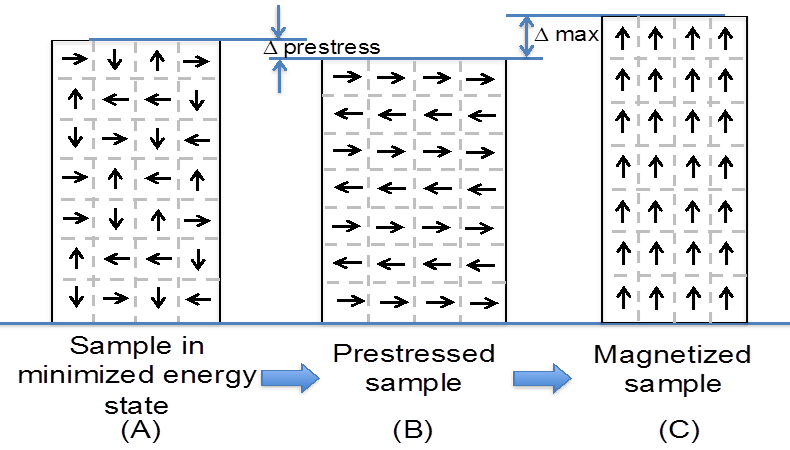
\includegraphics[width=0.5\textwidth]{prestressed-mag-anneal}
	\caption{Cartoons depicting a perfectly aligned cubic alloy with \hkl<100> magnetic easy axes as indicated. Arrows depict idealized orientation of magnetic domains.(A) Energy minimized state with closure domains randomly distributed throughout sample.  (B) Prestressed sample with aligned antiparallel magnetization vectors and sample length minimized due to stress-induced moment rotation. (C) Sample magnetized along length with $\Delta$max as the maximum achievable magnetostriction due to 90~$^{\circ}$ magnetic moment rotation.}
	\label{fig:prestressed-mag-anneal}
\end{figure}


Fe-Al is sufficiently magneto-elastic that coupling between bending stress and magnetic moment rotation yields readily observable time-varying magnetization changes in the alloy. In harvesters, power is generated in a copper coil that surrounds a magnetostrictive material when a time varying stress, e.g. vibration of the magnetostrictive material, produces a voltage in the coil (per Faraday’s law)\cite{Yoo2012}. Fe-Al is a body-centered cubic alloy textured to develop a  preferred orientation along the length of the strips by abnormal grain growth (AGG)\cite{Na2014,Na2014b,Na2013a}. The \hkl<100> directions are the magnetic easy axes. Subsequently, the stress annealing protocol was performed to introduce built-in uniaxial anisotropy perpendicular to the length of the strips\cite{Yoo2009}.  This was done to maximize 90$^{\circ}$ rotation of magnetic moments when the strip bends. Successful stress-anneal-induced magnetic anisotropy was achieved, but this stress annealing process could not provide uniform compressive stress on each tested sample leading to non-uniform magnetic flux change along the strip length. As a viable alternative for a uniform magnetic flux change, Brooks et al. have used magnetic field annealing to achieve nearly identical saturation magnetostriction under compressive and no preload values\cite{Brooks2012}. 





\subsection{Motivation}\label{abnormal-grain-growth}
%Describes Abnormal Grain Growth from Dr. Na's papers
%
Magnetostrictive Fe–Ga alloys (Galfenol) have promising attributes for application to sensors, actuators and energy harvesting as Clark et al. first reported in 2000\cite{clark2000magnetostrictive}. Single-crystal Galfenol has a body-centered
cubic (bcc) crystal structure, and along the \hkl<100> crystal orientations, it exhibits saturation magnetostriction of $\sim$400 ppm in low applied magnetic fields of $\sim$200 Oe. It also has a mechanical strength of $\sim$500 MPa, which is high relative to more costly rare earth magnetostrictive materials such as Terfenol-D alloys which exhibit giant magnetostriction ($\gtrsim$1600 ppm) but are brittle and require much higher magnetic fields ($\gtrsim$1000 Oe) for saturation\cite{clark2000magnetostrictive,Clark2003,Guruswamy2000}. The large magnetostriction and easy magnetization in single-crystal Galfenol alloys occur along the \hkl<100> orientation. It is thus desirable to obtain the \hkl<100> orientation in textured polycrystalline Galfenol, with the goal of providing enhanced mechanical properties and lower cost than single-crystal material, with similar magnetostrictive strain. 

%TODO: Insert paragraph about Alfenol properties and why they are good.


Two viable approaches have been employed to fabricate highly textured Fe–Ga alloys\cite{srisukhumbowornchai2001large,kellogg2003texture}. One is a directional solidification growth process, and the other is thermomechanical processing involving deformation via rolling and recrystallization through grain growth and orientation mechanisms. Currently, stress-annealed and field-annealed samples are first rolled into sheets from ingots, and then atmospherically annealed to develop large grains that cover over 90\% of the sample surface area. This process avoids lengthy and expensive single-crystal growth methods. We target Goss \hkl{110} and Cube \hkl{100} textures to obtain one and two directions, respectively, of easy magnetic axes and high magnetostriction in the plane of the rolled sheet.
 
%TODO: Connect AGG to surface energy

\subsubsection{Need for Surface Energy}

\textbf{Galfenol} 
%\textbf{Galfenol AGG is affected by sulfur surface segregation concentration}

We have been studying the development of Goss- and Cube-textured Galfenol rolled sheet as a low-cost alternative to magnetostrictive single crystal Galfenol for several years. We targeted Goss and Cube textures to obtain one and two directions respectively of easy magnetic axes and high magnetostriction in the plane of the rolled sheet. An additional benefit of developing a Cube texture is that it will make feasible use magnetic field annealing to maximize performance\cite{Yoo2008,Yoo2009} and thereby eliminate the need for stress annealing or use of prestress components in the design of devices that use these materials.\cite{Restorff2006,Summers2009b} Developing protocols for making thin sheet Galfenol with Goss or Cube textures has been challenging because the mechanisms that regulate grain boundary mobility and texture development in these alloys are not well understood. The preliminary results in Fig. \ref{fig:AGG-diagram} show AGG and texture development in Galfenol rolled sheet for several different anneal protocols. The dramatic difference in abnormal grain growth (AGG) and texture between the result in the top right image and the results in the two lower right images was accomplished by building on empirical insights from studies of Fe and Fe-Si alloys in which control of surface energy was used to regulate grain growth and ultimately to produce Cube-textured material.\cite{Walter1965,dunn1962surface,waeckerle1993effect,Kramer1992}

%TODO Insert paragraph explaining AGG and its roll in Galfenol/Alfenol magnetostriction
In other works, Kellogg et al. reported that binary Fe$_{0.83}$Ga$_{0.17}$ with a somewhat dispersed \hkl{001}\hkl<100> texture along rolling direction (RD) exhibited magnetostrictive strain of $\sim$160 ppm as a consequence of rolling and annealing at 1100$^{\circ}$C for 4 h\cite{kellogg2003texture}. Texture annealing of Fe$_{0.85}$Ga$_{0.15}$ alloy with 1 mol.\% NbC at 1150–1300$^{\circ}$C for 24 h changed the texture from a strong $\alpha$-fiber texture \hkl<110>$\parallel$RD in as-rolled sheet to a preferred texture with \hkl<100> orientation\cite{srisukhumbowornchai2004crystallographic}. In our prior work, we have demonstrated the texture development of Goss \hkl{011}\hkl<100> texture through secondary recrystallization by using NbC particles as an inhibitor of normal grain growth(NGG) \cite{Na2009}.


%\begin{figure}[h!] 
%	\centering
%	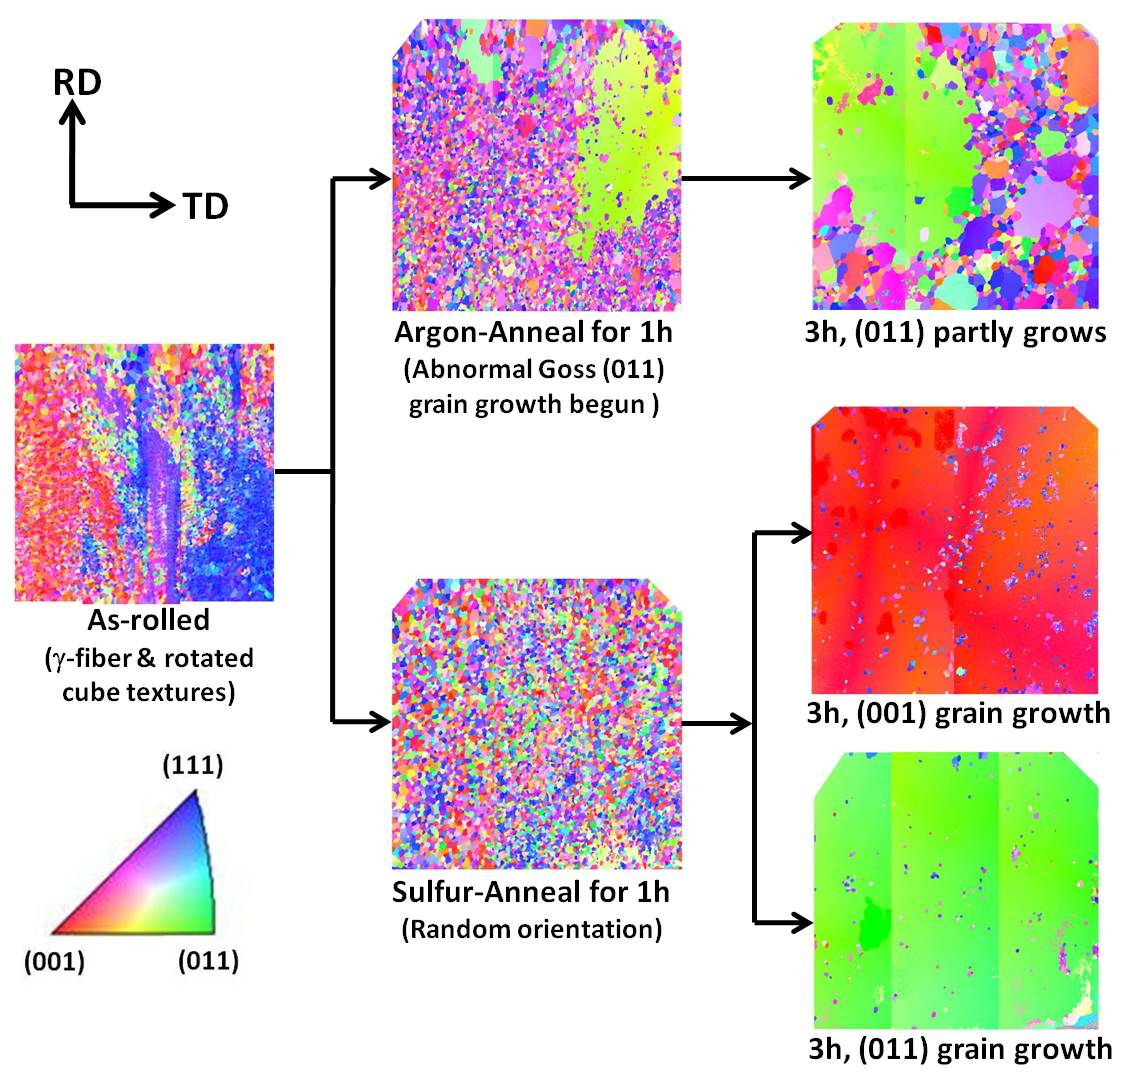
\includegraphics[width=0.6\textwidth]{AGG-diagram}
%	\caption{Diagram of AGG from as-rolled sample of (Fe-19$\%$Ga)+1.0$\%$NbC alloy (left) to argon- (upper) and sulfur-annealed (lower) samples for annealing times of 1h (middle) and 3h (right). EBSD images scanned along the normal direction of 12x12x0.45 mm$^{3}$ sheet. Red, green and blue indicate \hkl(001), \hkl(011) and \hkl(111) grains, respectively. 
%	}
%	\label{fig:AGG-diagram}		
%\end{figure}

In Fig. \ref{fig:AGG-diagram}, as-rolled polycrystalline Galfenol (left image) exhibits a strong $\gamma$-fiber and weak rotated cube textures, and starts with an $\alpha$-iron (B2) structure. A partly grown Goss texture developed over $\sim$39$\%$ of the sample surface area during a 3h argon-anneal (upper right image) due to grain boundary energy alone. We have also demonstrated that small variations in surface energy have a significant impact of the development of texture.\cite{Chun2010,Na2012b} The two lower right images show AGG with fully developed \hkl(001) and \hkl(011) grains over 90-95$ \% $ of the sample surface. AGG of (011) grains is very reproducible (insensitive to small variations in anneal conditions), while the development of (001) grains is challenging to produce/reproduce (highly sensitive to anneal conditions). Saturation magnetostriction values equal to 90$ \% $ and 
\begin{wrapfigure}[15]{l}{0.5\linewidth}
	\centering
	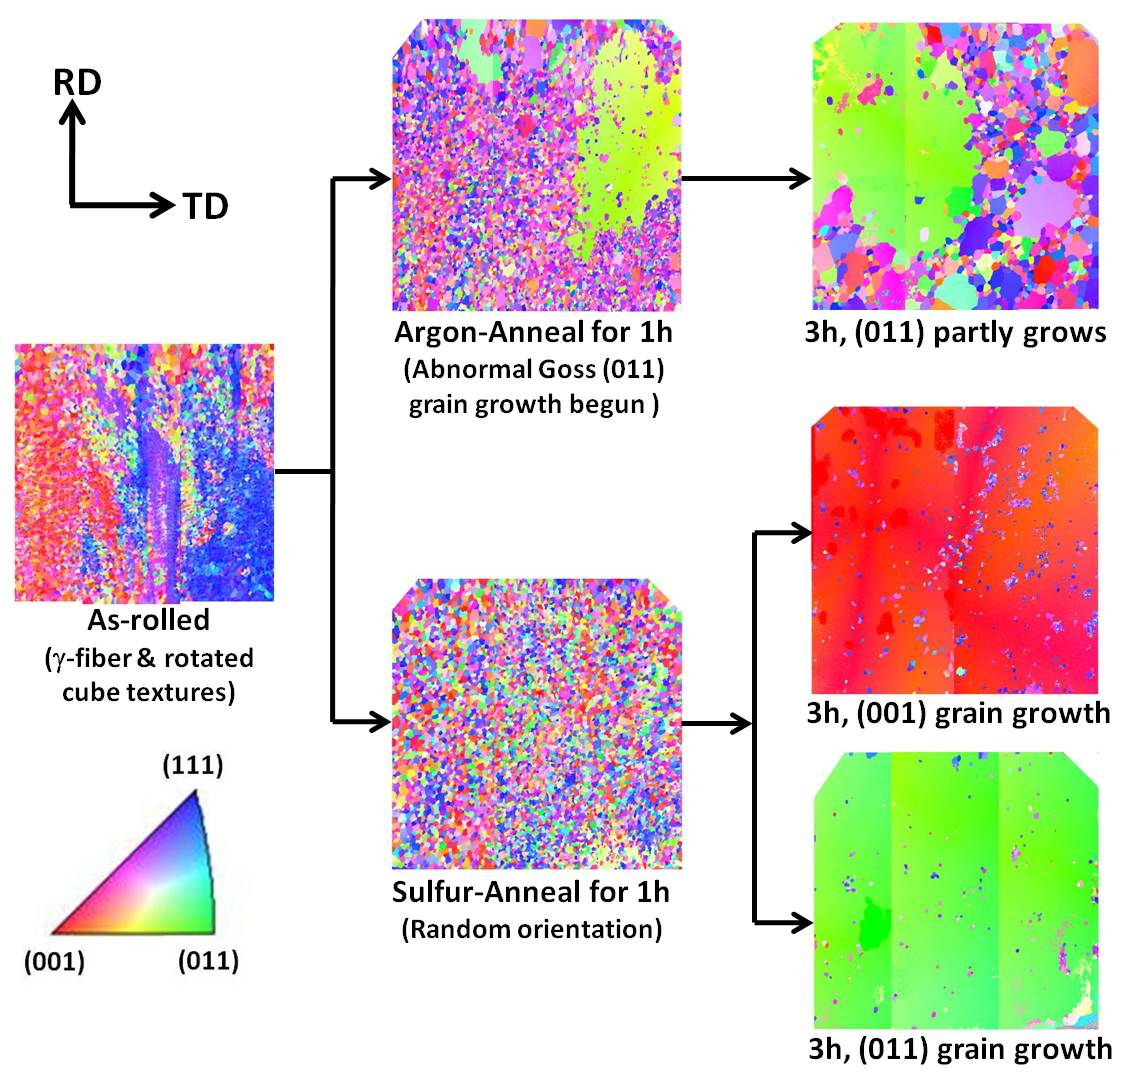
\includegraphics[width=0.45\textwidth,trim={0 0 0 0.5cm}]{AGG-diagram}
	\caption{Diagram of AGG from as-rolled sample of (Fe-19$\%$Ga)+1.0$\%$NbC alloy (left) to argon- (upper) and sulfur-annealed (lower) samples for annealing times of 1h (middle) and 3h (right). EBSD images scanned along the normal direction of 12x12x0.45 mm$^{3}$ sheet. Red, green and blue indicate \hkl(001), \hkl(011) and \hkl(111) grains, respectively. 
	}
	\label{fig:AGG-diagram}	
\end{wrapfigure}
 84$ \% $ of single crystal \hkl(100) values for alloy of the same composition were measured in sulfur-annealed samples with \hkl(001) and \hkl(011) grain growth, respectively.  


Figure \ref{fig:AGG-diagram} results are the first and only that we know of to employ concepts that date back to the mid-1960’s \cite{Walter1965,dunn1962surface,waeckerle1993effect} for developing AGG in irons, Fe-Si and silicon-steels together with Kramer’s work in the 1990’s\cite{Kramer1992} on control of surface energy to develop Cube texture in Fe-Si. Our research hypothesis is motivated by our desire to understand the physical metallurgy that lead to these results and be able to routinely reproduce these results in rare-earth-free anisotropic alloys. \\
\textbf{Alfenol}

The importance of Alfenol surface energy lies in the Aerosmart Lab's need for more efficient energy harvesting materials. Goss-textured Alfenol can reach magnetostrictive constants of ~184 ppm, and the elusive Cube-textured Alfenol would reach even higher magnetostriction values due to the additional direction of easy magnetic axes. An added benefit of developing a Cube texture is that it will make feasible use of magnetic field annealing to maximize performance\cite{Yoo2009,Yoo2008} and thereby eliminate the need for stress annealing or use of pre-stress components in the design of devices that use these materials\cite{Restorff2006,Summers2009}. Clearly, Alfenol AGG is affected differently than Galfenol under sulfur concentrations. This must be due to the differences in orientation-dependent surface energy between Galfenol and Alfenol.
	


 Magnetostrictive Fe–Ga alloys (Galfenol) have promising attributes for application to sensors, actuators and energy harvesting as Clark \etal first reported in 2000\cite{clark2000magnetostrictive}. Galfenol has a body-centered cubic (bcc) crystal structure, and along the \hkl<100> crystal orientations, it exhibits saturation magnetostriction of $\sim$400 ppm in low applied magnetic fields of $\sim$200 Oe. It also has a mechanical strength of $\sim$500 MPa, which is high relative to more costly rare earth magnetostrictive materials. Terfenol-D alloys exhibit giant magnetostriction ($\gtrsim$1600 ppm) but are brittle and require much higher magnetic fields ($\gtrsim$1000 Oe) for saturation\cite{clark2000magnetostrictive,Clark2003,Guruswamy2000}. The large magnetostriction and easy magnetization in Galfenol alloys occur along the \hkl<100> orientation. It is thus desirable to obtain the \hkl<100> orientation in textured polycrystalline Galfenol, with the goal of providing enhanced mechanical properties and lower cost than single-crystal material, while preserving magnetostrictive strain. 

%TODO: Insert paragraph about Alfenol properties and why they are good.
%TODO: CORRECTION -> will insert paragraph about Alfenol if necessary. 



 Two viable approaches have been employed to fabricate highly textured Fe–Ga alloys\cite{srisukhumbowornchai2001large,kellogg2003texture}. One is a directional solidification growth process, and the other is thermomechanical processing involving deformation via rolling and recrystallization through grain growth and  
\begin{figure}[h]
	\centering
	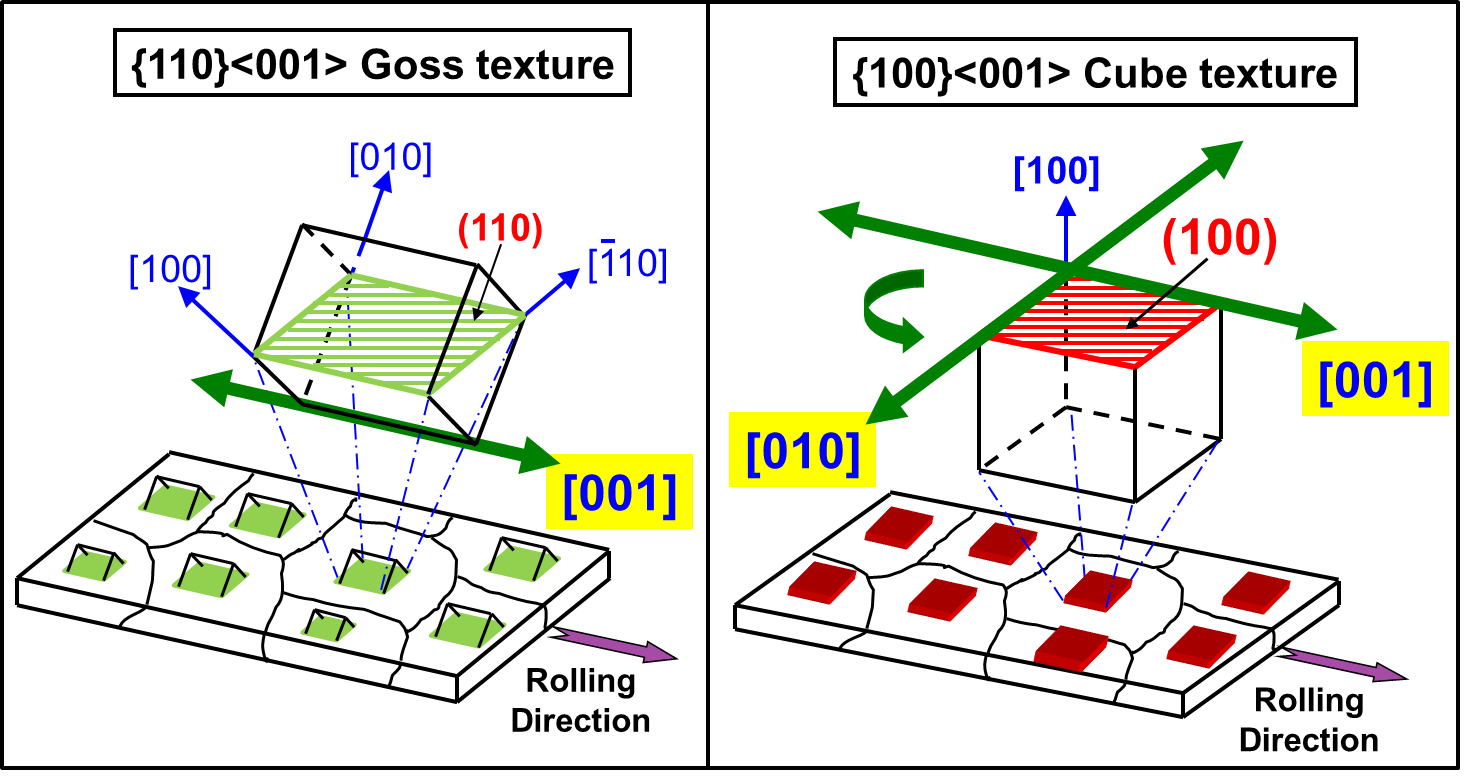
\includegraphics[width=0.8\textwidth,trim={0 0 0 0.5cm}]{goss_cube}
	\caption{This is an illustration of Goss and Cube textures shown with their respective axes of easy magnetization. Goss has one easy axis, and Cube has two easy axes.}
	\label{fig:goss_cube}	
\end{figure}
 orientation mechanisms. Development of a uniform texture over 90\% of the surface has been achieved when samples are first rolled into sheets from ingots, and then atmospherically annealed to develop large grains on the sample surface area by utilizing the abnormal grain growth (AGG) phenomenon.\cite{Na2012a,Na2014}


 AGG is often detrimental in piezoelectric ceramics because it lowers the hardness and the larger developed grain sizes lead to degradation of the piezoelectric effect.\cite{Bing2014} For the Aerosmart group's application goals, AGG is advantageous for targeting Goss \hkl{110} and Cube \hkl{100} textures to obtain one and two directions, respectively, of easy magnetic axes and high magnetostriction in the plane of rolled sheets. This process avoids lengthy and expensive single-crystal growth methods while still producing Galfenol with sufficient magnetostrictive properties for device application. We have been studying the development of Goss- and Cube-textured Galfenol rolled sheet as a low-cost alternative to magnetostrictive single-crystal Galfenol for several years. To optimize specific grain growth, we have  incorporated pinning particles during the rolling process, experimented with different annealing temperatures and times, and modified the annealing environment.\cite{Na2007b,Na2008,Na2009,Na2012} 

 EBSD images spatially map crystal orientations on well-polished specimen by using backscattered electron patterns from the electron beam in a scanning electron microscope (SEM). From these patterns, we can use statistical tools to measure average misorientation, grain size, and crystallographic texture. Figure \ref{fig:AGG-diagram} depicts electron backscatter diffraction (EBSD) images of more successful annealing conditions we have tested. As-rolled polycrystalline Galfenol (left image) exhibits a strong $\gamma$-fiber \hkl<111>$ \parallel $ND (normal direction to the sheet surface) and weak rotated cube textures, and starts with an $\alpha$-iron (B2) structure. A partly grown Goss texture developed over $\sim$39$\%$ of the sample surface area during a 3h argon-anneal (upper right image) due to grain boundary energy alone. This is because large inert argon particles do not react with the Galfenol surface, and do not modify the surface energy. We have demonstrated that small variations in surface energy have a significant impact of the development of texture.\cite{Chun2010,Na2012b} The two lower right images show AGG with fully developed \hkl(001) and \hkl(011) grains over 90-95$ \% $ of the sample surface. 
\begin{wrapfigure}[14]{l}{0.5\linewidth}
	\centering
	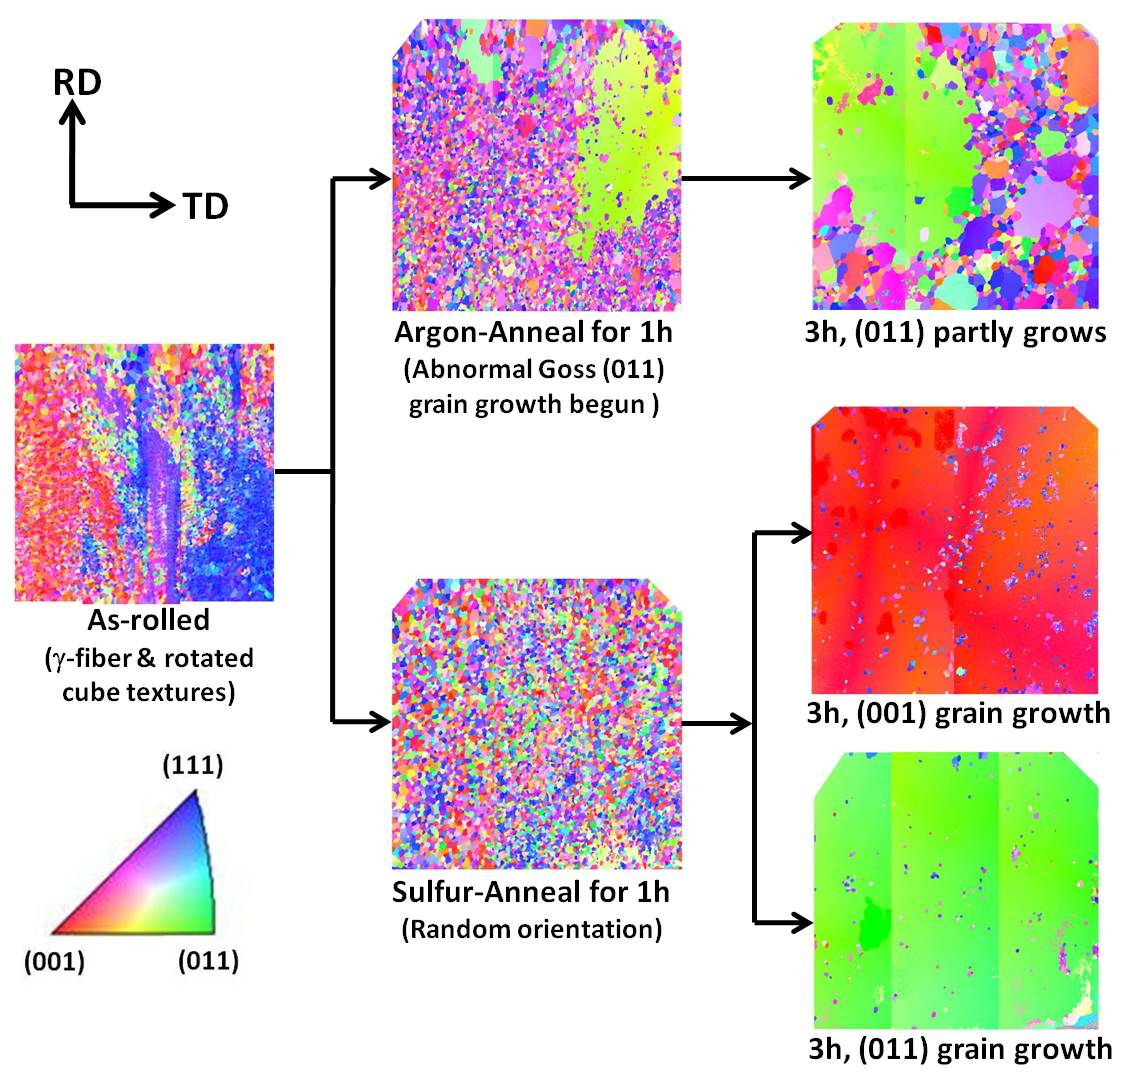
\includegraphics[width=0.45\textwidth,trim={0 0 0 0}]{AGG-diagram}
	\caption{Diagram of AGG from as-rolled sample of (Fe-19$\%$Ga)+1.0$\%$NbC alloy (left) to argon- (upper) and sulfur-annealed (lower) samples for annealing times of 1h (middle) and 3h (right). EBSD images scanned along the normal direction of 12x12x0.45 mm$^{3}$ sheet. Red, green and blue indicate \hkl(001), \hkl(011) and \hkl(111) grains, respectively. 
	}
	\label{fig:AGG-diagram}	
\end{wrapfigure}
 AGG of (011) grains are very reproducible and insensitive to small variations in anneal conditions, while the development of (001) grains are challenging to produce/reproduce due to highly sensitive to anneal conditions. Saturation magnetostriction values equal to 90$ \% $ and 84$ \% $ of single-crystal \hkl(100) values for alloy of the same composition were measured in sulfur-annealed samples with \hkl(001) and \hkl(011) grain growth, respectively.  

 Developing protocols for making thin sheet Galfenol with Goss or Cube textures has been challenging because the mechanisms that regulate grain boundary mobility and texture development in these alloys are not well understood. Modeling techniques that examine grain boundary interactions, coincident site lattice (CSL) and high energy grain boundary (HEGB), have been investigated to understand AGG mechanisms. These techniques sufficiently describe abnormally grown Goss grains in \fegacomp(x=19)+1.0 mol\% NbC rolled sheets, but mechanisms for abnormally grown Cube-grains are still not understood.\cite{Chun2010} We believe these models are insufficient because extraneous driving forces caused by the control of surface energy from atmospheric annealing conditions, as described by Kramer \etal, are not properly incorporated. By characterizing the surface energy of specific Galfenol grains, we can develop a more accurate thermodynamic-based framework for modeling AGG and texture development that will be used to understand why a high temperature atmospheric anneal transforms myriad crystallite grains into the highly textured, single-crystal-like polycrysalline material. 

%Figure \ref{fig:AGG-diagram} results are the first and only that we know of to employ concepts that date back to the mid-1960’s \cite{Walter1965,dunn1962surface,waeckerle1993effect} for developing AGG in irons, Fe-Si and silicon-steels together with Kramer’s work in the 1990’s\cite{Kramer1992} on control of surface energy to develop Cube texture in Fe-Si. Our research hypothesis is motivated by our desire to understand the physical metallurgy that lead to these results and be able to routinely reproduce these results in rare-earth-free anisotropic alloys. 



%\subsubsection{Need for Surface Energy}

%\textbf{Galfenol} 
%\textbf{Galfenol AGG is affected by sulfur surface segregation concentration}

 

%An additional benefit of developing a Cube texture is that it will make feasible use magnetic field annealing to maximize performance\cite{Yoo2008,Yoo2009} and thereby eliminate the need for stress annealing or use of prestress components in the design of devices that use these materials.\cite{Restorff2006,Summers2009b} The preliminary results in Fig. \ref{fig:AGG-diagram} show AGG and texture development in Galfenol rolled sheet for several different anneal protocols. The dramatic difference in abnormal grain growth (AGG) and texture between the result in the top right image and the results in the two lower right images was accomplished by building on empirical insights from studies of Fe and Fe-Si alloys in which control of surface energy was used to regulate grain growth and ultimately to produce Cube-textured material.\cite{Walter1965,dunn1962surface,waeckerle1993effect,Kramer1992}



%In other works, Kellogg et al. reported that binary Fe$_{0.83}$Ga$_{0.17}$ with a somewhat dispersed \hkl{001}\hkl<100> texture along rolling direction (RD) exhibited magnetostrictive strain of $\sim$160 ppm as a consequence of rolling and annealing at 1100$^{\circ}$C for 4 h\cite{kellogg2003texture}. Texture annealing of Fe$_{0.85}$Ga$_{0.15}$ alloy with 1 mol.\% NbC at 1150–1300$^{\circ}$C for 24 h changed the texture from a strong $\alpha$-fiber texture \hkl<110>$\parallel$RD in as-rolled sheet to a preferred texture with \hkl<100> orientation\cite{srisukhumbowornchai2004crystallographic}. In our prior work, we have demonstrated the texture development of Goss \hkl{011}\hkl<100> texture through secondary recrystallization by using NbC particles as an inhibitor of normal grain growth(NGG) \cite{Na2009}.


%\begin{figure}[h!] 
%	\centering
%	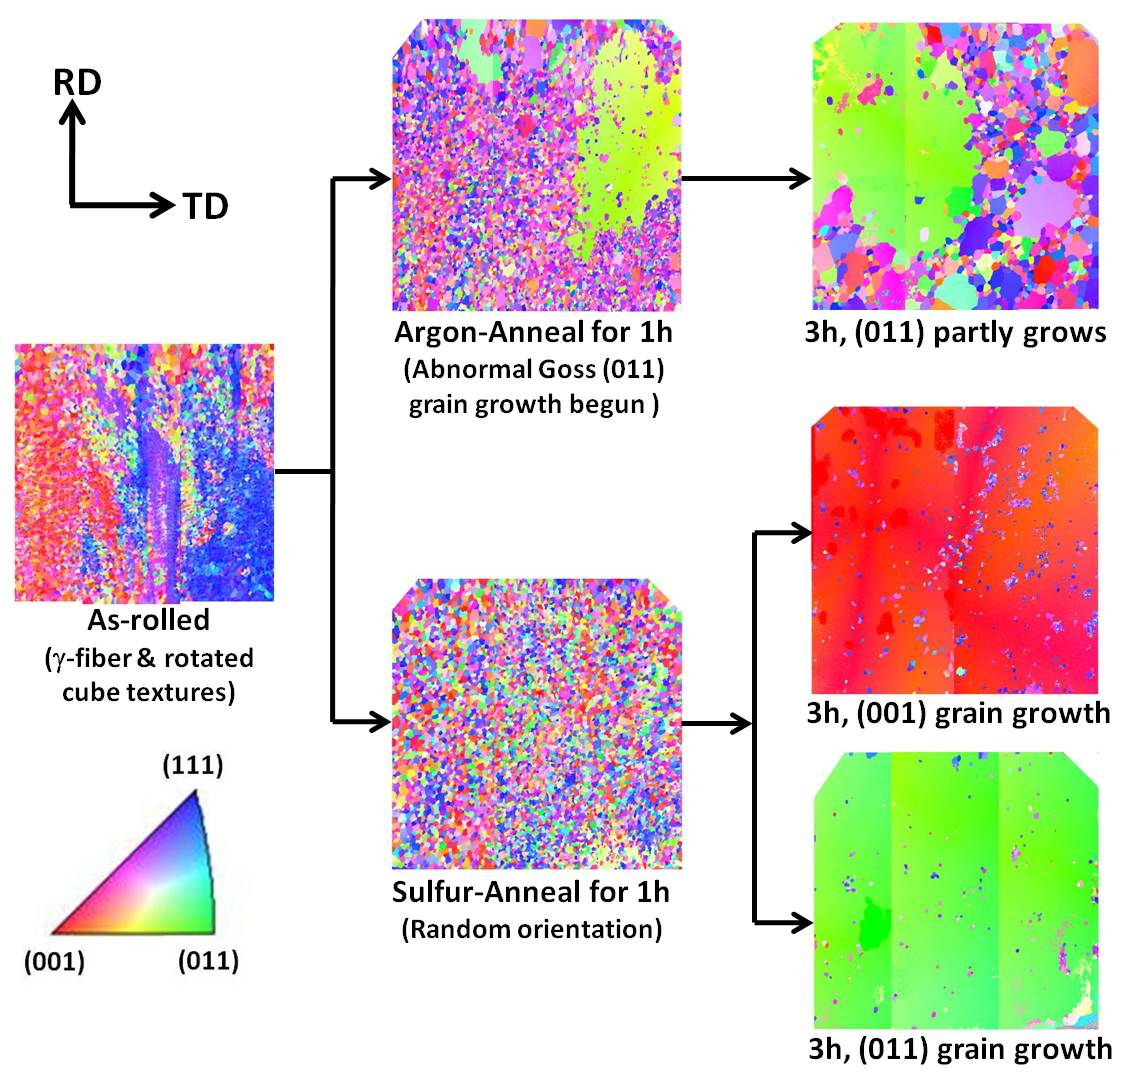
\includegraphics[width=0.6\textwidth]{AGG-diagram}
%	\caption{Diagram of AGG from as-rolled sample of (Fe-19$\%$Ga)+1.0$\%$NbC alloy (left) to argon- (upper) and sulfur-annealed (lower) samples for annealing times of 1h (middle) and 3h (right). EBSD images scanned along the normal direction of 12x12x0.45 mm$^{3}$ sheet. Red, green and blue indicate \hkl(001), \hkl(011) and \hkl(111) grains, respectively. 
%	}
%	\label{fig:AGG-diagram}		
%\end{figure}




%\textbf{Alfenol}

%TODO: Take this paragraph to the end as a future work thing. "This research has the potential for extension to other systems. Specifically, for ou
%The importance of Alfenol surface energy lies in the Aerosmart Lab's need for more efficient energy harvesting materials. Goss-textured Alfenol can reach magnetostrictive constants of ~184 ppm, and the elusive Cube-textured Alfenol would reach even higher magnetostriction values due to the additional direction of easy magnetic axes. An added benefit of developing a Cube texture is that it will make feasible use of magnetic field annealing to maximize performance\cite{Yoo2009,Yoo2008} and thereby eliminate the need for stress annealing or use of pre-stress components in the design of devices that use these materials\cite{Restorff2006,Summers2009}. Clearly, Alfenol AGG is affected differently than Galfenol under sulfur concentrations. This must be due to the differences in orientation-dependent surface energy between Galfenol and Alfenol.


%\subsection{Surface Energy}\label{surface-energy}

\subsubsection{Defining Surface Energy}\label{define-surf-energy}
%TODO: Rewrite entire section in your own words in order to not copyright the author below. 
%\textbf{Interface Science and Composites (Chapter 3: Solid-Liquid Interface), by Soo-Jin Park and Min-Kang Seo\cite{Park2011a}}


 Thermodynamically, the physical origin of the surface free energy is the excess Gibbs free energy of matter at the interface. There is a negative free energy change when two flat surfaces, A and B, are brought into adhesive contact in a medium. Israelachvili describes this as twice the interfacial energy $ \gamma_{AB} $ of the A-B interface, which is positive by convention,\cite{Israelachvili2011n} as seen in Equation \ref{SFE}.
\begin{equation}\label{SFE}
	\Delta W = -2\gamma_{AB}
\end{equation}
 In principle, Equation \ref{SFE} can be used to calculate the surface tension of a condensed phase held together by the long-range forces. 

 The interaction of a liquid with a solid is characterized by the term "wetting." Wetting can be understood as the spreading of a liquid over a solid surface. One way to quantify a liquid's surface wetting characteristics is to measure the contact angle of a drop of liquid placed on the surface of an object. The profile of contact angle formed by the solid-liquid and liquid-vapor interfaces are measured from the side of the liquid. 
 The wetting ability of a liquid is a function of the surface energy of the solid-vapor interface, the liquid-gas interface, and the solid-liquid interface. The surface energy across an interface is a measure of the energy required to form the unit area of a new surface at the interface. The intermolecular bonds, or cohesive forces, between the molecules of a liquid cause surface tension. When the liquid encounters another substance, there is usually an attraction between the two materials. The adhesive forces between the liquid and the second substance will compete against the cohesive forces of the liquid.  Liquids with strong cohesive bonds and weaker adhesive forces will tend to bead-up or form a droplet when in contact with another material. Liquids with relatively weak cohesive bonds and a strong attraction to another material will tend to spread over that material. Here, the energetically favorable outcome is the formation of adhesive bonds, such is the case with water droplets on high-surface energy metal substrates.
 
 \begin{wrapfigure}[8]{R}{0.5\linewidth}
 	\centering
 	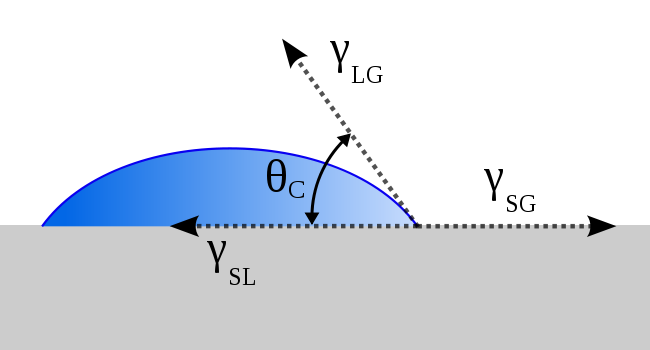
\includegraphics[width=0.5\textwidth,trim={0 0 0 2cm}]{Contact_angle}
 	\caption{This illustration shows a vector representation of the interfacial tensions involved in a solid-liquid-gas contact angle experiment. [Image available in public domain: wikimedia.org]}
 	\label{fig:ca-vector}
 \end{wrapfigure}

 %Depending on the thermodynamic state or the hydrodynamic status of the liquid drop in which the contact angle is measured, two types of contact angels can be defined. If the contact angle is measured when either the liquid drop contines to spread or when its thermodynamic state conditions continue to change, the measured contact angle is termed the dynamic contact angle. However, if the contact angle is measured under conditions in which the liquid drop is stationary and the surrounding conditions in which the liquid drop is stationary and the surrounding conditions are in the steady state, the measured contact angle is known as the static/equilibrium contact angle. The contact angle technique is chosen for studies of the wettability phenomena owing to its simplicity. 


 The solid-liquid interface plays a fundamental role in diverse fields and helps with an understanding of physical phenomena and structural knowledge of the interface at the atomic scale. Fields of interest include catalysis, lubrication, electrochemistry, colloidal systems, biological reactions, and, most relevantly, crystal growth. 

 Contact angle measurements, as described by Thomas Young in 1805, remain the most accurate method for determining the interaction energy between a liquid (\textit{L}) and a solid (\textit{S}). A contact angle is defined geometrically as the angle formed by a liquid at the three-phase boundary, where vapor, liquid, and solid intersect. The magnitude of a contact angle can be directly correlated to the magnitude of liquid cohesion energy, $\gamma_{L}$, and the energy of adhesion between a liquid and solid. Young described the equilibrium contact angle at the three-phase boundary in terms of the vectorial sum, as shown in Figure \ref{fig:ca-vector}, resulting in an equilibrium force balance. The famous Young's equation (Equation \ref{young_eqn}) is derived in Appendix \ref{appendixA} from the Gibbs free energy at equilibrium. 


\hypertarget{youngeqn}{}
\begin{equation}\label{young_eqn}
	\boxed{\gamma_{SV} =\gamma_{SL}-\gamma_{LV}\cos\theta}	
\end{equation}
%\end{tcolorbox}
 %We attempt to model a new contact angle method based on Equation \ref{young_eqn} in Section \ref{section2}

\subsection{Preliminary investigations}
There are currently no experimental methods available to measure surface energies associated with different crystallographic orientations of metals. High temperature methods involving cylindrical metal samples and destructive methods involving drop shape samples of a targeted liquid metal near the melting point are available for measuring surface energy of amorphous and isotropic solid metals.\cite{Egry2010,Aqra2011,Cao2011} For glass and polymeric solids with relatively low surface energies, the water-drop method has been shown to be effective for the determination of surface energy at room temperature.\cite{Ahadian2010,Kwok2000,Tavana2005} A previous group member, Hyunsuk Chun, attempted to use the water drop method for contact angle measurements on \hkl(001), \hkl(011) and \hkl(111) facets of 17.9$\%$Ga Galfenol single-crystal samples using facilities at NIST.\cite{Costa2016} Averaging  water contact angles in air on \hkl(001), \hkl(011) and \hkl(111) facets from 20-30 measurements resulted in 72.$\pm$5.3\degree, 87.01$\pm$5.4\degree, and 63.11\degree, respectively. These measurements were used to estimate surface energy using the Girifalco–Good–Fowkes–Young (GGFY) equation, $\gamma_{LV} (1+\cos\theta) = 2 \sqrt{\gamma_{LV}\gamma_{SV}}$. Determined values of \gamSV for each facet ($ \gamma_{001} $= 0.0277 J/m$^2$, $\gamma_{011}$ = 0.0199 J/m$^2$, $\gamma_{111}$ = 0.0380 J/m$^2 $) are too small to be correct. The values are about two orders of magnitude smaller than expected when compared to values of $\alpha$-iron DFT calculations ($\gamma_{100}$ = 2.6660 J/m$^2$, $\gamma_{110}$ = 2.0535 J/m$^2$, $\gamma_{111}$ = 2.5271 J/m$^2$).\cite{Wang2000} A water contact angle in air works well for estimating surface energy of solids with magnitudes less than water surface tension ($\gamma_W$ $\sim$ 72 mJ/m$^2$), and fails for metallic solids, where the drop surface tension is several orders of magnitude lower than that of metals. 


\subsubsection{Thermal Grooving}

The thermal grooving technique was considered as a possible approach to understanding the interactions between adjacent grains in Galfenol that we target for AGG. Annealed samples were polished and re-annealed to develop thermal grooves. EBSD identified where \hkl(100), \hkl(110), and \hkl(111) orientations met on each sample. By measuring the dihedral angle formed at these grain boundaries, the ratio of grain boundary energy and surface energy was calculated according to the following equation: 
\begin{equation}
\frac{\gamma_{GB}}{\gamma_{S}} = 2\cos\left(\frac{\Psi_{S}}{2}\right) 
\end{equation}
where $\gamma_{GB}$ is the grain boundary energy, $\gamma_{S}  $ is the surface energy, and $\Psi_{S} $ is the dihedral angle, as described in Rohrer \etal\cite{Rohrer2010a} The most symmetric thermal groove came from a \hkl(110)/\hkl(111) grain boundary on a rolled and annealed (Fe-19\%Ga)+1.0\%NbC sample made 
\begin{figure}[h!]
	\centering
	\begin{subfigure}[c]{0.45\textwidth}
		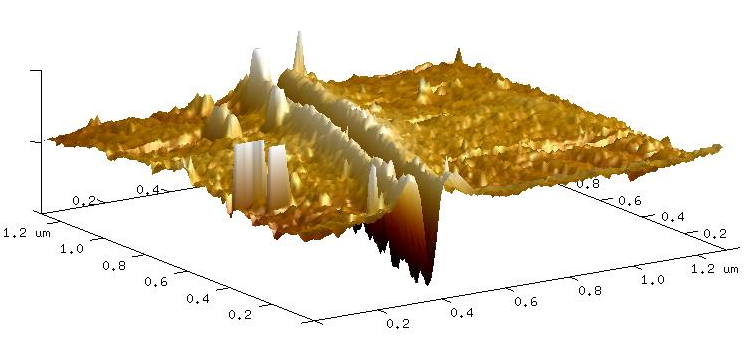
\includegraphics[width=\linewidth]{afm-groove-fega}
		\subcaption{~}
		\label{fig:afm-groove-fega}		
	\end{subfigure}
	\begin{subfigure}[c]{0.45\textwidth} 
		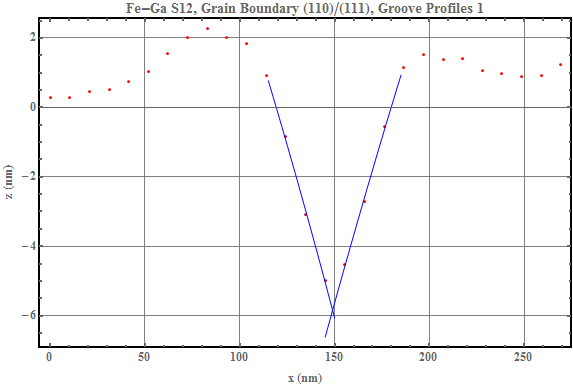
\includegraphics[width=\linewidth]{fega-groove-profile}
		\subcaption{~}
		\label{fig:fega-groove-profile}		
	\end{subfigure}
	\caption{(a) 3D rendering of (110)/(111) grain boundary on surface of  for (Fe-19\%Ga)+1.0\%NbC sample where the depth of groove is ~8 nm. (b) A quadratic fit of a (110)/(111) grain boundary profile for a (Fe-19\%Ga)+1.0\%NbC sample.}
	\label{fig:thermal-groove}
\end{figure}
by Suok-Min Na, as seen in the Figure \ref{fig:thermal-groove}.  The grain boundary profiles were measured using atomic force microscopy (AFM), and the dihedral angles were extrapolated from the profiles using both AFM software by Bruker and a quadratic fit.  The results are shown in Table \ref{groove-analysis}. This groove in particular had a depth of $\sim$8 nm which is significantly smaller in depth compared to grooves of other metal alloys.\cite{Skidmore2004a} Relative energies between 1/4 and 1/2 are expected for metals, but this unusually small groove might explain why we see high variation in dihedral angles. 
%Many of the grain boundary grooves were not suitable for measuring based on their lack of symmetry at the grain boundary interface. 
To properly analyze the thermal grooving technique, an extensive grain boundary study of the effect annealing temperatures and times have on Galfenol would need to be investigated. While this may be an interesting avenue of research in the future, the resultant calculations of relative grain energies do not contribute to the ultimate goal of achieving a comprehensive AGG model for Galfenol. Realization of this project's goal lies in the measurement of orientation-dependent surface energy using contact angle measurements. 


\begin{table}[h!]
	\centering
	\caption{Calculated dihedral angles and relative energies from our most symmetric grain boundary groove.}
	\begin{tabular} { |p{1cm}||c|c|c|c|  } 
		\hline
		\multicolumn{5}{|c|}{fe-ga-s12-006 profile analysis - GB (110)/(111)}\\
		\hline
		~	&\multicolumn{2}{|c|}{Bruker Software}		&\multicolumn{2}{|c|}{Quadratic Fit}	\\
		\hline
		Profile	&Dihedral Angle (\degree)	&Relative Energy	&Dihedral Angle (\degree)	&Relative Energy \\ 
		\hline
		1		&156.957	&0.399471	&151.253	&0.496475	\\
		\hline
		2		&156.244	&0.411657	&157.093	&0.397144	\\
		\hline
		3		&154.402	&0.443063	&155.554	&0.423432	\\
		\hline
		4		&157.221	&0.394955	&152.785	&0.470541	\\
		\hline
		5		&154.732	&0.437445	&154.966	&0.433458	\\
		\hline
		6		&158.386	&0.375003	&154.482	&0.441706	\\
		\hline
		\textbf{Avg}	&156.324~$\pm$1.529	&0.410266 $\pm$0.0261178	&154.356 $\pm$2.069	&0.443793 $\pm$0.0351932\\
		\hline
	\end{tabular}
	\label{groove-analysis}
\end{table}

%\subsubsection{Defining Surface Energy}\label{define-surf-energy}
%TODO: Rewrite entire section in your own words in order to not copyright the author below. 
%\textbf{Interface Science and Composites (Chapter 3: Solid-Liquid Interface), by Soo-Jin Park and Min-Kang Seo\cite{Park2011a}}


Thermodynamically, the physical origin of the surface free energy is the excess Gibbs free energy of matter at the interface. Atoms or molecules exposed at an interface are surrounded by fewer neighbors, such as solid, liquid, and gas phases, resulting in an anisotropic distribution of these neighbors, which is the characteristic of a surface. Interaction energy must be shared between phases with the neighboring molecules. Hence, the surface free energy, $\gamma$, represents the rate of change of the Gibbs free energy of the system with respect to the area, $A$, at a constant pressure and temperature\cite{Chattoraj2012}:
\begin{equation}\label{SFE}
	\gamma = \left(\frac{\partial G}{\partial A}\right)_{T,P}
\end{equation}
In principle, Equation \ref{SFE} can be used to calculate the surface tension of a condensed phase held together by the long-range forces. 

The interaction of a liquid with a solid is characterized by the term "wetting." Wetting can be understood as the spreading of a liquid over a solid surface, the penetration of a liquid into porous materials, or the displacement of one liquid by another. This phenomenon can help to characterize a surface, and to determine the interaction between a solid and a liquid. 

One way to quantify a liquid's surface wetting characteristics is to measure the contact angle of a drop of liquid placed on the surface of an object. The contact angle formed by the solid-liquid and liquid-vapor interfaces are measured from the side of the liquid. Liquids wet surfaces when the contact angle is less than 90\degree. For a penetrant material to be effective, the contact angle should be as small as possible. In fact, the contact angle for most liquid penetrants approach 0\degree. 

The wetting ability of a liquid is a function of the surface energy of the solid-vapor interface, the liquid-gas interface, and the solid-liquid interface. The surface energy across an interface or the surface tension at the interface is a measure of the energy required to form the unit area of a new surface at the interface. The intermolecular bonds, or cohesive forces, between the molecules of a liquid cause surface tension. When the liquid encounters another substance, there is usually an attraction between the two materials. The adhesive forces between the liquid and the second substance will compete against the cohesive forces of the liquid.  Liquids with strong cohesive bonds and weaker adhesive forces will tend to bead-up or form a droplet when in contact with another material. Liquids with relatively weak cohesive bonds and a strong attraction to another material, or the desire to create adhesive bonds, will tend to spread over the material, such is the case with water droplets on high-surface energy metal substrates.

Depending on the thermodynamic state or the hydrodynamic status of the liquid drop in which the contact angle is measured, two types of contact angels can be defined. If the contact angle is measured when either the liquid drop contines to spread or when its thermodynamic state conditions continue to change, the measured contact angle is termed the dynamic contact angle. However, if the contact angle is measured under conditions in which the liquid drop is stationary and the surrounding conditions in which the liquid drop is stationary and the surrounding conditions are in the steady state, the measured contact angle is known as the static/equilibrium contact angle. The contact angle technique is chosen for studies of the wettability phenomena owing to its simplicity. 

The solid-liquid interface plays a fundamental role in diverse fields and helps with an understanding of physical phenomena and structural knowledge of the interface at the atomic scale. Fields of interest include catalysis, lubrication, electrochemistry, colloidal systems, biological reactions, and, most relevantly, crystal growth. Therefore, unravelling the atomic structure at the solid-liquid interface is one of the major challenges. 
\begin{wrapfigure}[8]{R}{0.5\linewidth}
	\centering
	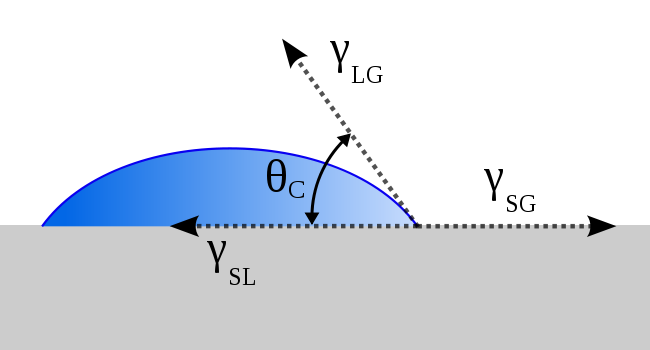
\includegraphics[width=0.5\textwidth,trim={0 0 0 2cm}]{Contact_angle}
	\caption{This illustration shows a vector representation of the interfacial tensions involved in a solid-liquid-gas contact angle experiment. [Image available in public domain: wikimedia.org]}
	\label{fig:ca-vector}
\end{wrapfigure}

Contact angle measurements, as described by Thomas Young in 1805, remain the most accurate method for determining the interaction energy between a liquid (L) and a solid (S) in a condensed state at the minimum equilibrium distance of S and L. This is defined geometrically as the angle formed by a liquid at the three-phase boundary, where vapor, liquid, and solid intersect. It measures the result of liquid cohesion energy, in the guise of $\gamma_{L}$ and the energy of adhesion between a liquid and solid. Young described the equilibrium contact angle at the three-phase boundary in terms of the vectorial sum, as shown in Figure \ref{fig:ca-vector}, resulting in an equilibrium force balance. The famous Young's equation is derived from the Gibbs free energy at equilibrium, as seen from the result of Equation \ref{young_eqn}. 



%TODO: put derivation in an Appendix

\begin{equation}\label{young_eqn}
	\boxed{\gamma_{SV} =\gamma_{SL}-\gamma_{LV}\cos\theta}	
\end{equation}
%\end{tcolorbox}
We attempt to model a new contact angle method based on Equation \ref{young_eqn} in Section \ref{section2}

%\subsubsection{\textbf{Insula}}
%Surfaces have energy associated with them because work is needed to form them. Surface energy is the work per unit area done by the force that creates the new surface.
%
%In the bulk, atoms are evenly surrounded and the cohesive forces between the atoms tend to balance. On the surface there are atoms on one side only, so there is a net inward cohesive force. This creates a force on the surface that tries to minimise its area. When considered as a force rather than an energy, the force is called "surface tension".
%
%As temperature increases, the atoms in a solid vibrate more, and reduce the cohesive force binding the atoms. The surface energy depends on the net inward cohesive force and so surface energy decreases with increasing temperature. The surface energy for many metals (e.g. Ag, Au, and Cu) goes down by about 0.5 mJ/(m$^{2}\cdot K$) with increasing temperature. Water goes down by about 160 mJ/(m$^{2}\cdot K$).
%
%\subsubsection{\textbf{Wikipedia}}
%%TODO: Find citations from this snippet
%The energy of the bulk component of a solid substrate is determined by the types of interactions that hold the substrate together. High energy substrates are held together by bonds, while low energy substrates are held together by forces. Covalent, ionic, and metallic bonds are much stronger than forces such as van der Waals and hydrogen bonding. High energy substrates are more easily wet than low energy substrates.[5] In addition, more complete wetting will occur if the substrate has a much higher surface energy than the liquid.[6]
%
%Many techniques can be used to enhance wetting. Surface treatments (such as Corona treatment and acid etching) can be used to increase the surface energy of the substrate.[7][8] Additives can also be added to the liquid to decrease its surface energy. This technique is employed often in paint formulations to ensure that they will be evenly spread on a surface.[9]




The interactions of water with a low-energy and high-energy solid surface differ significantly. The relative energy of a solid compared to a liquid has to do with the bulk nature of the solid. Solids with weak molecular crystals (e.g., fluorocarbons, hydrocarbons, etc.) where the molecules are held together by weak physical forces (e.g., van der Waals and hydrogen bonds) are termed low-energy solids. A very low input of energy is required to break these solids, thus they typically have surface energy values $<$72 mJ/m$^2$.  Metals, glasses, and ceramics are known as "hard solids" because the chemical bonds that hold them together (e.g., covalent, ionic, or metallic) are very strong. Thus, these surfaces are high-energy because of the high amount of energy needed to break these solids to make two new surfaces, (e.g. see Equation \ref{SFE} in Section \ref{define-surf-energy}). High energy solids typically have surfaces energies $>$72 mJ/m$^2$.  The threshold between these two types of surfaces lies in their surface energy values relative to the surface tension of water, $\sim$72 mJ/m$^2$. Water tends to partially wet a low energy surface and completely wet a high energy surface based on how much lesser or greater the surface energy of the solid is compared to water, respectively. 

I will investigate two approaches to overcome the challenges involved in measuring the surface energy of metals using contact angle measurements in the next two chapters. The first will study temperature variations of Galfenol surface energy using a droplet of gallium as the probe liquid. Gallium is a liquid at room temperature with a surface tension that is roughly one order of magnitude higher than that of water: $\gamma_{Ga}\sim$715.3 mJ/m$^2$. It is expected that a measurable contact angle will form between Galfenol and liquid gallium, and this information will be incorporated into an analytical model to extract the solid surface energy. The second will build on the two-liquid-phase technique to form a measurable water contact angle on the surface of Galfenol. To supplement this measurement, Galfenol samples will be patterned with a planned surface geometry to increase the water contact angle and properly determine the Young's contact angle to be used in surface energy calculations. Both experiments will use highly Goss textured Galfenol as well as single-crystal Galfenol samples to assure isotropic crystal orientation for contact angle measurements. 

Once experimental results are validated with published values, DFT predictions of the surface energy associated with different crystallographic orientations in Fe-Ga will be tested and verified. This task and the resultant capability should have broad applicability beyond the needs of this dissertation for extension to polycrystalline textured metals and thin films.
%This method has the potential to become a valuable tool for obtaining empirical surface energy data associated with AGG of Galfenol grains as well as other metallurgical studies.
%/research that lack experimental verification of surface energy around room temperature. 
%


\newpage
\chapter{Gallium Drop Contact Angle Experiment}\label{chapter2}


This chapter will focus on the gallium drop contact angle experiment. Its theory, development, results, and thoughts on improvement in future studies. 





\section{Theory behind model}\label{section2-1}

\subsection{thesis proposal}

\begin{figure}
	\centering
	\begin{subfigure}[b]{0.7\textwidth}
		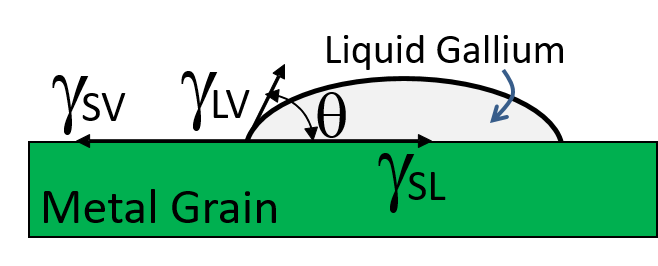
\includegraphics[width=\textwidth,trim={0 0 0 2cm}]{youngs-ga}
	%	\caption{Interfacial tensions on Ga drop on solid surface}
		\label{fig:youngs-ga}
	\end{subfigure}
	%add desired spacing between images, e. g. ~, \quad, \qquad, \hfill etc. 
	%(or a blank line to force the subfigure onto a new line)
	\begin{subfigure}[b]{0.7\textwidth}
		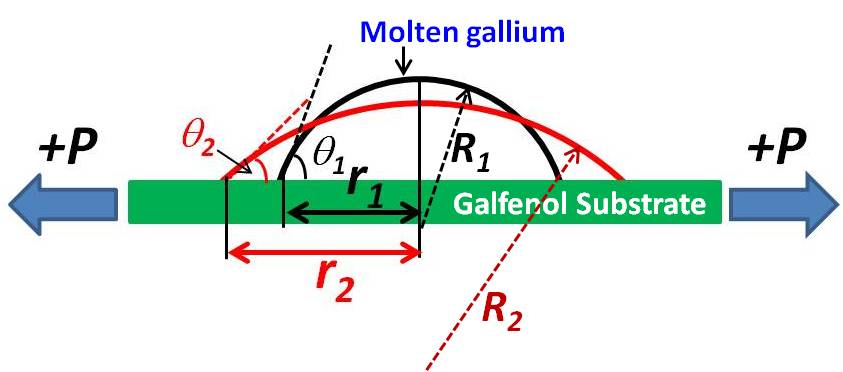
\includegraphics[width=\textwidth,trim={0 2cm 0 0}]{thermal-expand-drop}
	%	\caption{Thermal expansion of drop}
		\label{fig:thermal-expand-drop}
	\end{subfigure}
	\caption{Schematics indicating notation used and contact angles $\theta_{i}$, radii of drop-solid contact area $r_{i}$, and radii of curvature for a spherical drop $R_{i}$, for two temperatures as thermal expansion induced tension $P$ strains the substrate.}
	\label{fig:therm-exp-ga}
\end{figure}
The gallium drop contact angle technique uses classic contact angle measurement techniques and drop size analysis on a liquid metal, gallium, resting on a metal surface as the metal is heated. Figure \ref{fig:therm-exp-ga} illustrates the experiment. Gallium was chosen as the probe liquid for our high surface energy metals, \gamSV $\sim$2000 mJ/m$^2$, because it is a liquid above 29.8\degree C and it has an average surface tension of $\gamma_{Ga}\sim$715.3 mJ/m$^2$.\cite{Hardy1985} This means that liquid Ga will not completely wet a bare metal surface as water does. Water has a relatively low surface tension, $\gamma_{water}\sim$72.0 mJ/m$^2$, compared to a solid metal surface energy, hence when interacting with a bare metal surface the water contact angle will reduce to zero, and no solid surface energy can be calculated, which can be seen in Equation \ref{young_eqn}. The surface tension of Ga varies by 5 mJ/m$^2$ in the temperature range that this experiment will be carried out, $\sim$30-100\degree C, and will be accounted for in the final surface energy calculation. Ga surface tension can be linear plotted as $\gamma_{Ga} = 709 - 0.066(T-29.8)$, where $T$ is the temperature and 29.8 is the melting point of Ga.\cite{Hardy1985} A plot of Ga surface tension vs. temperature from Hardy \etal is shown in Figure \ref{fig:se-vs-temp-ga}. 

%%%%%%%%%%%%%%%%%%%
%This paragraph explains the choice of gallium as a probe liquid in a contact angle experiment for a metal surface instead of water. 
%It establishes Ga as a main contributor to the experiment. One that must be characterized well. 
%%%%%%%%%%%%%%%%%%%


\begin{figure}
	\centering
	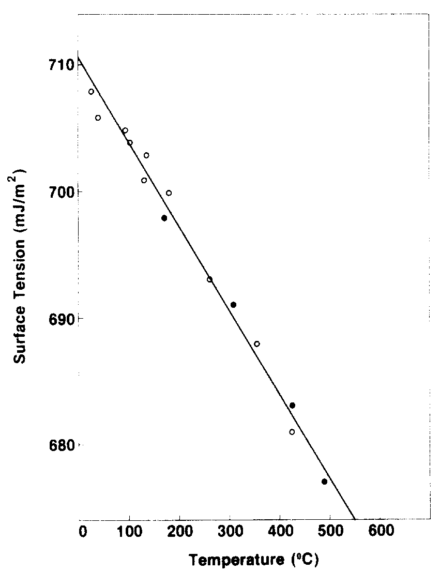
\includegraphics[width=0.5\linewidth,trim={0 0 0 1cm}]{se-vs-temp-ga}
	\caption{This figure plots the surface tension of pure Ga as temperature increases. This figure is from Hardy \etal \cite{Hardy1985}.}
	\label{fig:se-vs-temp-ga}
\end{figure}


Surface energy of FeGa will be calculated at temperatures ranging from 30-100\degree C in 10\degree C intervals. Changes in surface energy are introduced by thermal expansion of the substrate. By expanding the distance between atoms at the surface of the solid, the solid surface energy decreases. Intuitively, this makes sense because as the metallic bond distance increases, the less energy it would take to break those bonds. Electrons will begin to localize around the nuclei, as the attractive forces between atoms will decrease with the increased atomic separation. Ultimately, it will become easier for the metal to cleave and form two new surfaces, hence the surface energy decreases as temperature increases. 

Since a heated sample thermally expands, we can say that there is a tensile force on the edges of the stationary droplet of Ga. The triple point at every point of the droplet contact radius expands outward due to the thermal expansion of the probed surface. This tensile load can be called $ +P(T) $, seen in Figure \ref{fig:therm-exp-ga}, which effectively appears as a uniform radial force of the planar solid surface as temperature increases. By slowly heating the system by $\sim$1\degree C/min, the substrate expands uniformly while equilibrating at each temperature. Hence, terms due to variation in thermal energy and variation of the total Gibbs free energy are negligible. 

The surface energy of the substrate as a function of temperature, $\gamma_{SV}(T)$, can be related to $ +P(T) $ through the changes in the liquid Ga drop contact angle $\theta$, the radius $ r $ of the liquid gallium drop in contact with the metal surface, and the height $ h $ of the droplet hemisphere. A video system is used to precisely quantify dimension changes in substrate and liquid metal drop during thermal expansion.
%%%%%%%%%
%this paragraph introduces the model of finding solid surface energy from the gallium drop experiment. 
%
%As temperature is increased, a force is exerted on the triple line of the gallium sessile drop by the thermal expansion of the substrate.
%%%%%%%%%

The interfacial energy between the substrate solid and the liquid gallium drop, \gamSL, can be written as \gamSL$=P(T)/2\pi r$. The uniform tension introduced by thermal expansion of substrate can be expressed as:
\begin{equation}\label{uniform-tension}
	P(T) = E_{sub}\alpha_{sub}(T-T_{mp})
\end{equation}
where $T_{mp}$ is the melting temperature of gallium, $E$  is the substrate Young’s modulus, and $\alpha$ is the linear thermal expansion coefficient. A linear function can be used to write the gallium-air interfacial tension a function of temperature, \gamLV $= a-b(T-T_{mp})$, where \textit{a} and \textit{b} are positive constants found experimentally.\cite{Hardy1985,Alchagirov2005} Putting the terms for \gamSL and \gamSV into \hyperlink{youngeqn}{Young’s equation}\cite{Rudawska2009,Tadmor2004}:
\begin{equation*}%\label{youngs-eqn-ga1}
	\gamma_{SV} =  \frac{E_{sub}\alpha_{sub}(T-T_{mp})}{2\pi r} + \left[a-b(T-T_{mp})\right]\cos\theta
\end{equation*}
%%%%%%%%%%%%%%%%%%%%%
%Fully derives the gallium drop surface energy equation.
%This paragraph needs to be partially combined with the previous paragraph. 
%%%%%%%%%%%%%%%%%%%%%


A relationship between the variable radius $r(T)$ associated with the area of the circular region of solid-liquid contact $A_{SL}(T)$, the contact angle $\theta(T)$ and the volume $V$ of the spherical cap formed by the drop is derived next. To determine the radius $r(T)$, the geometric relationships based on the radius of curvature $R(T)$ of a sphere is mapped onto the hemispherical liquid cap. The drop is modeled as being part of a sphere whose radius is $R(T)$. It is assumed that he volume $V$ of the drop is the volume of the spherical cap, and remains constant. The radius $R(T)$ can then be expressed in terms of the volume and the angle:
\begin{equation*}\label{drop-geom}
	R(T) = V^{1/3} \left[\frac{\pi}{3} \left(2-3\cos\theta(T)+\cos^{3}\theta(T)\right)\right]^{-1/3}
\end{equation*}
Using the relation $r(T)=R(T)\sin\theta(T)$ (i.e. $\theta=$0\degree corresponds to complete wetting of the surface and at $\theta=90$\degree,  $r=R$) the following formula for surface energy as a function of temperature $T$ and contact angle $\theta(T)$ (shown as $\theta_{T}$) is:
\begin{equation}\label{youngs-eqn-ga}
	\gamma_{SV} =  \underbracket{\frac{E_{sub}\alpha_{sub}(T-T_{mp})}{2\pi}\left[\frac{\pi\left(2-3\cos\theta_{T}+\cos^{3}\theta_{T}\right)}{3V\sin^{3}\theta_{T}} \right]^{1/3}}_{\text{\gamSL(T)}} + \underbracket{\left[a-b(T-T_{mp})\right]}_{\text{\gamLV(T)}} \cos\theta_{T}
\end{equation}
This gives the surface energy \gamSV of specific grains as a function of temperature by measuring $T$ and $\theta$ at thermal equilibrium.





\section{Preliminary experiments}\label{section2-2}
In order to perform contact angle measurements on any material, the surface of that material must be pristine and well characterized. There can be no doubt that the probed surface is free of debris, organics, or oxides, for the case of metals, lest the contact angle be influenced by something other than the probed material. Proper sample storage and chemical cleaning (acetone $\Rightarrow$ methanol $ \Rightarrow $ DI rinse $ \Rightarrow $ N$_2$ dry) is satisfactory for removing particulates and organic residue, but exposing a bare metal surface by removing the native oxide layer is challenging. This chapter provides basic oxide removal techniques, but there is a more detailed oxide removal study in Chapter \ref{chapter3}. 
The surface must also be as close to atomically flat as possible. Most literature will approximate their surfaces as flat as long as the roughness is 10$^2$ greater than the contact area radius. 

One of the challenges in developing this new surface energy measurement capability is the need to expose the surface of the metal substrate that is shielded by surface oxides. The following strategies for removing the oxide layer and preventing  natural oxidation, thereby increasing the accuracy of measurement, will be employed independently and in combination:
\begin{outline}
	\1 A flux used in high-temperature metal joining processes plays roles of dissolving of the oxides on the metal surface and preventing of re-oxidation as a chemical agent.
	\1 Colloidal silica polishing with nano-sized particles, such as is used for precise surface observations, like EBSD scans, which require clean surfaces to accurately detect patterns.
	\1 Electro-polishing is effective for passivation of clean surfaces after chemical and mechanical polishing for removal of surface oxides. 
\end{outline}
%Results using the proposed approach were to be validated through comparison of results for oriented single crystals with published theoretical values for pure metal elements of a specific crystallography (e.g. Ni, Cu, Fe)  and comparison with experimental data from amorphous metals (e.g. Vitreloy or liquid steel) with destructive high temperature methods for measuring surface energy. 
It should be noted that all of these techniques will not prevent oxides from forming for an extended period of time. Therefore, the cleaning would have to be followed by isolation in high vacuum, an inert environment, or another liquid environment that prevents oxidation.

\subsection{Sample Preparation}
\subsubsection{Rolling and annealing}
Single crystal ingots were prepared by DOE Ames Laboratory, most likely using the Czochralski Method. Polycrystalline samples are prepared in the Aerosmart lab by Dr. Suok-Min Na using a progressive hot, warm, then cold rolling technique from a polycrystalline Galfenol ingot. The annealing process is described in \hyperlink{abnormal-grain-growth}{Chapter 1}. Single crystal samples are preferred for contact angle experiments because the prepared surface is isotropic, therefore multiple locations on a single sample surface can be probed and compared as equal surfaces. 


\subsubsection{Polishing}


Samples were prepared by manual grinding with incrementally higher grit SiC paper up to 1200 fine grit and then fine polishing using silica gel with 60 nm sized particles to minimize the roughness as well as the stressed surface states created during grinding.\cite{Hoffmann1987} Roughness measurements were performed on ten different 1$\mu$m x 1$\mu$m areas with an atomic force microscope (Veeco Dimension 3100) after fine polishing. Surface roughness values of ~1 nm were measured, thus there is minimal roughness influence on the contact angle measurements. Below are AFM images showing the difference between 1200 fine polishing and subsequent silica gel polishing. 
\begin{figure}
	\centering
	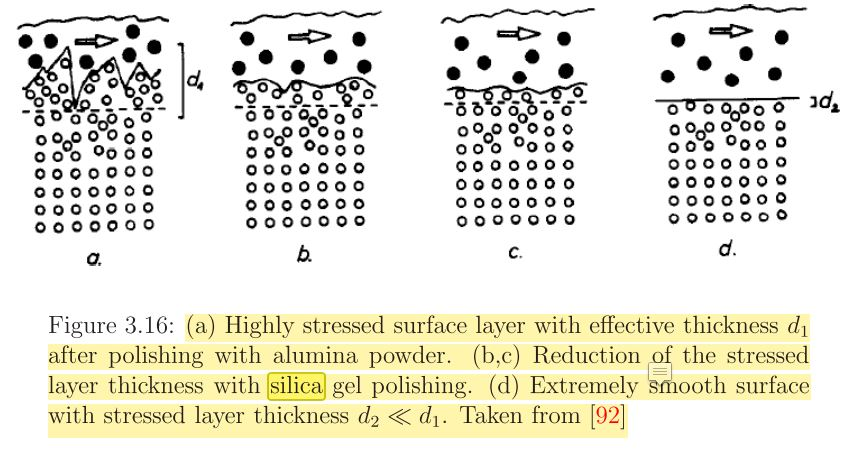
\includegraphics[width=\linewidth,trim={0 0 0 1cm}]{silica-polish}
	\caption{}
	\label{fig:silica-polish}
\end{figure}


%TODO insert an AFM image here to show roughness after a silica polish



\subsubsection{Electron Backscatter Diffraction}
%TODO Insert highly-textured polycrystal sample EBSD image made near beginning of project. 

%TODO single crystal EBSD images for (100), (110), and (111) samples that were vibratory polished
\subsubsection{Atomic Force Microscopy}
%TODO Expand on why AFM is a good enough calculator of roughness at a nanoscale. 

AFM is one of the simplest ways to determine roughness at the sub-nanometer scale, as opposed to profilometry which tends to lack the $<$100 nm resolution.

\subsection{Thermal Chamber Design Progression}
\subsubsection{Contact Angle Goniometer (Verison 1)}
Preliminary designs of my contact angle goniometer implement a radiative temperature control box which encloses an argon gas filled container where the sample resides, as seen in Figure \ref{fig:rad-temp-box}.  The presence of argon is meant to prevent any further oxidation of the Galfenol sample as well as the gallium droplet. The container was initially made of a clear acrylic plastic, but prolonged exposure to temperatures above 80\degree C caused thermal deformation of the plastic making longer experiments impossible to perform without environment contamination.  A clear pyrex container replaced the acrylic box to fix this issue.  Application of the liquid gallium drop to our surfaces was done via a mounted plastic syringe with disposable stainless steel hypodermic needles that were available at the time. Liquid gallium tends to adhere strongly to the stainless steel needle tips which makes wetting to the sample very difficult. The stainless steel tip tends to deform the highly viscous gallium drop resulting in non-uniform hemispheric drop shapes, as shown in Figure \ref{fig:deformed-ga}.
\begin{figure}[h]
	\centering
	\begin{subfigure}[c]{0.45\textwidth}
		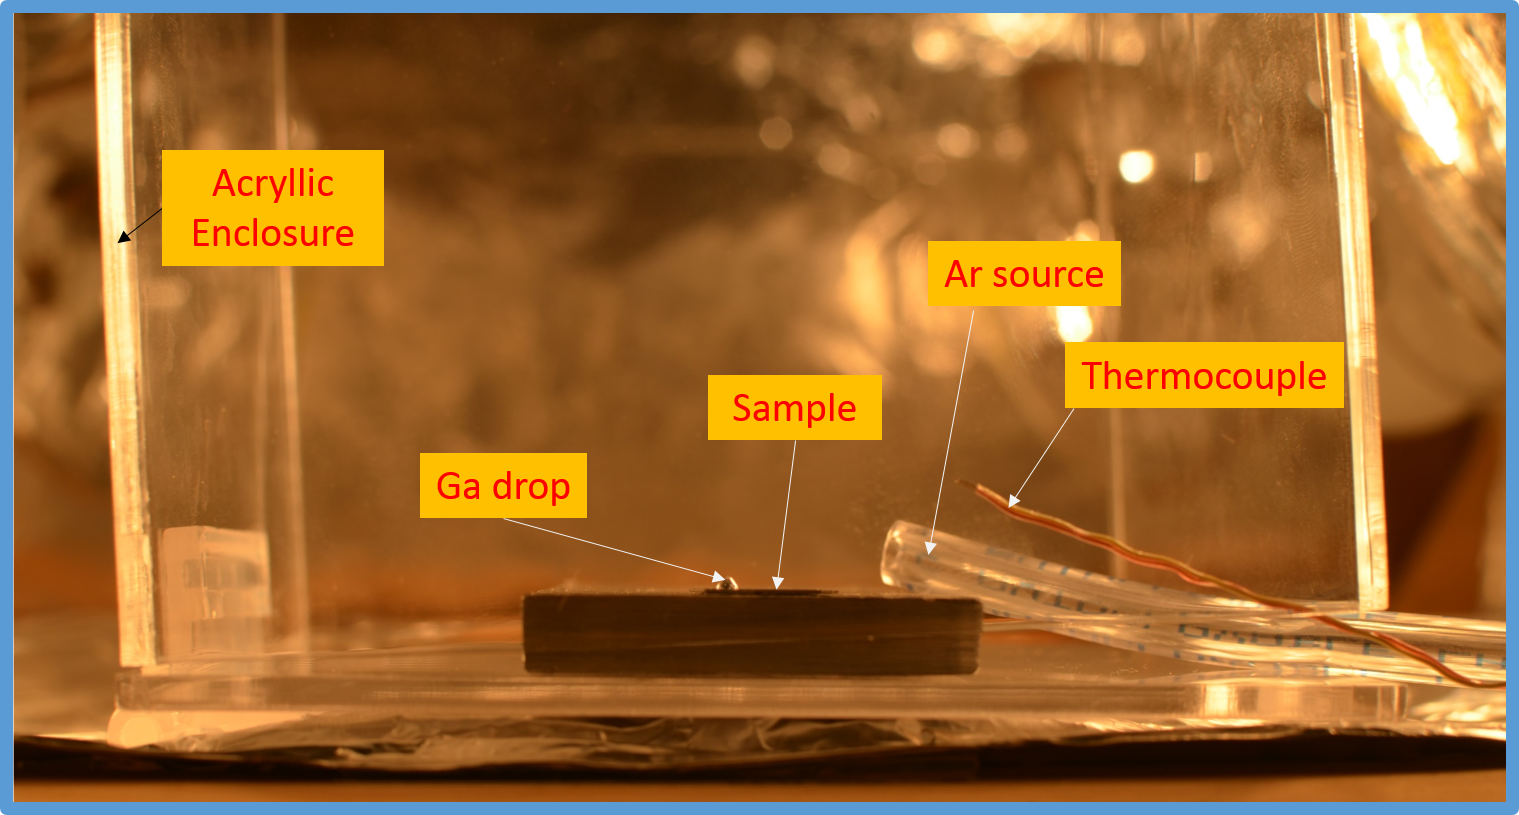
\includegraphics[width=\linewidth]{rad-temp-box}
		\subcaption{~}
		\label{fig:rad-temp-box}		
	\end{subfigure}
	\begin{subfigure}[c]{0.45\textwidth} 
		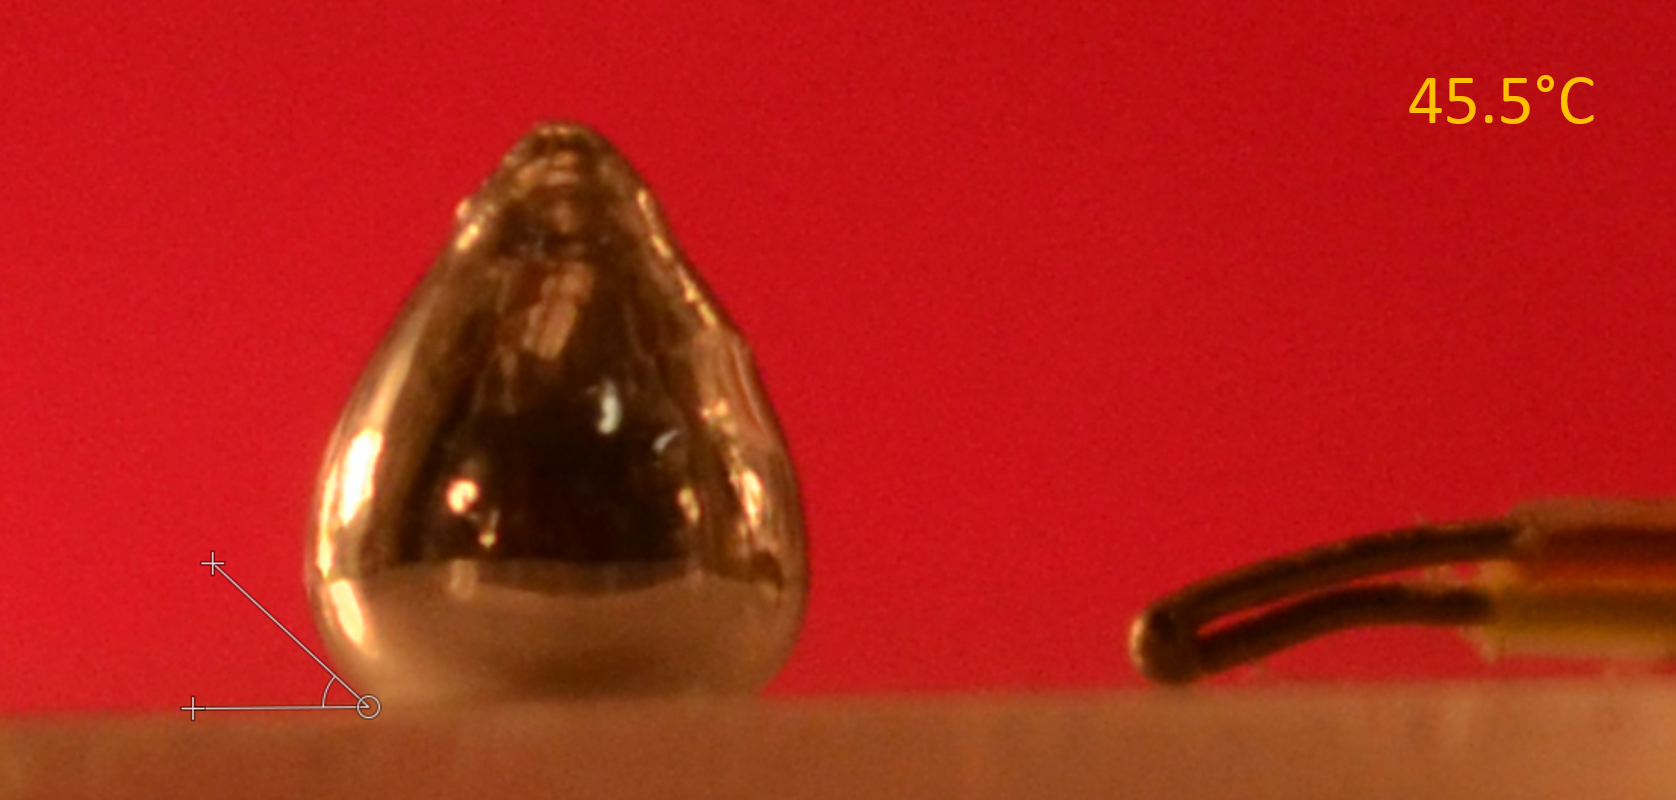
\includegraphics[width=\linewidth]{deformed-ga}
		\subcaption{~}
		\label{fig:deformed-ga}		
	\end{subfigure}
	\caption{(a) The first design of our contact angle goniometer.  The acrylic container houses the argon environment and sample.  This design was modified with a more stable glass enclosure. (b) A highly deformed gallium drop next to the thermocouple on a ceramic YAG test sample at 45.5\degree C. The angle measured on this droplet was subtracted from 180\degree since it was not measured through the liquid.}
	\label{fig:prelim-design}
\end{figure}



%\begin{figure}
%	\centering
%		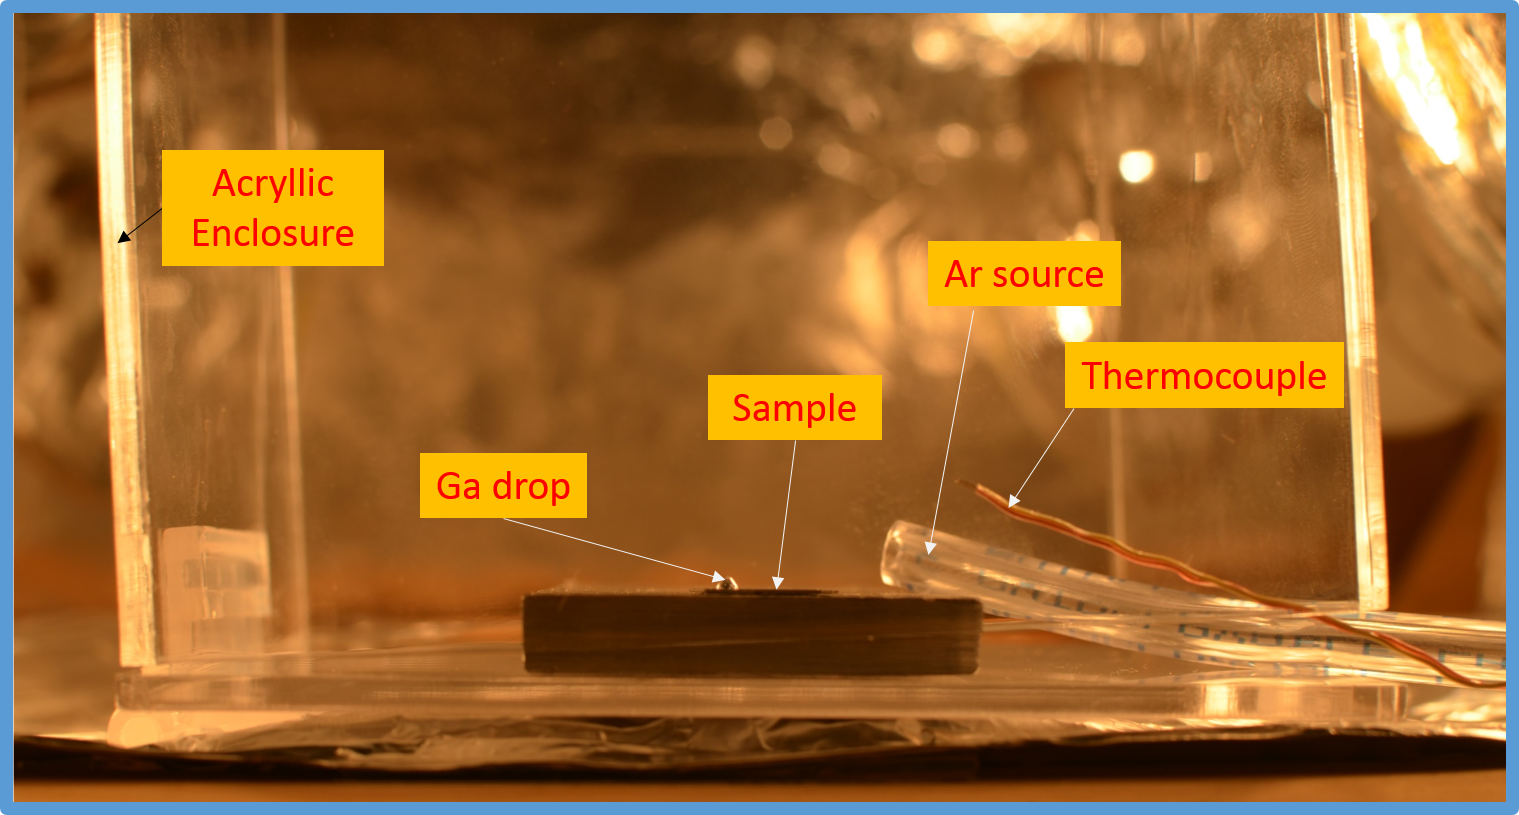
\includegraphics[width=\linewidth]{rad-temp-box}
%	\caption{(a) The first design of our contact angle goniometer.  The acrylic container houses the argon environment and sample.  This design was modified with a more stable glass enclosure. (b) A highly deformed gallium drop next to the thermocouple on a ceramic YAG test sample at 45.5\degree C.}
%	\label{fig:prelim-design}
%\end{figure}
The radiative box that housed this experiment had a high variability in temperature according to thermocouple readings, so a smaller apparatus with a top-side syringe opening is made to properly perform gallium drop tests at specific temperatures and prevent interaction with the experiment environment. There must also be bright white backlighting to obtain a high contrast drop profile. In this radiative box configuration, the high-reflecting liquid metal surface prevents a high contrast drop profile image, as seen in Figure \ref{fig:deformed-ga}. Proper contact angle measurements also require the gallium droplets to carefully wet the surface while forming an axisymmetric and spherical-like shape on the solid surface. A height adjustment system must be used to move the gallium pendant drop close enough to the sample surface for solid adhesive forces to overcome the adhesion to the needle. Lastly, the argon gas environment could be more well contained, instead of just filling up the glass sample enclosure from the bottom and spilling out the top due to higher density argon displacing the surrounding air environment. 

\subsubsection{Version 2}
\begin{figure}
	\centering
	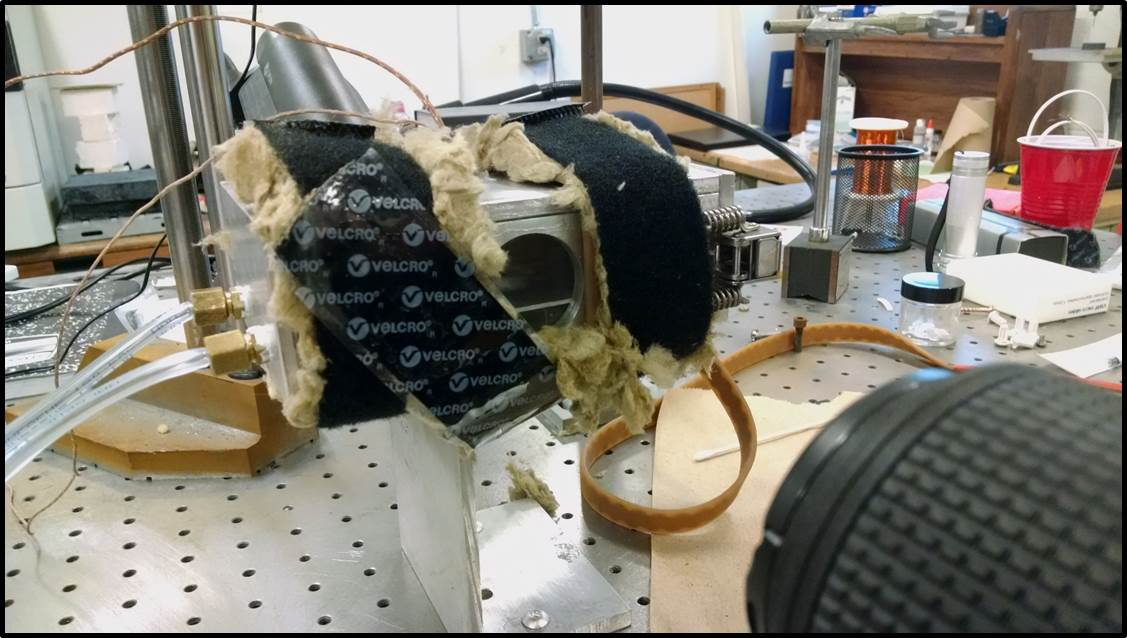
\includegraphics[width=\linewidth,trim={0 0 0 1cm}]{enviro_chamber}
	\caption{The second version of our gallium contact angle goniometer. The aluminum enclosure conductively transfers heat, the gas lines flow Ar gas into the chamber, top-mounted thermocouples monitor the gas and sample temperature, and the glass windows allow for backlighting of the drop profile along with high resolution image capture using a DSLR camera.}
	\label{fig:enviro_chamber}
\end{figure}
The new experimental apparatus can be seen in Figure \ref{fig:enviro_chamber}. The main structure is made of aluminum with two round glass windows on the front and back. The aluminum is meant to conductively transfer heat to the substrate by means of a heating cable wrapped around the outside of the structure. The high thermal conductivity of aluminum allows for a quick transfer of heat, thus an increased control of sample temperature. The time percentage dial controller attached to the heating tape is calibrated with the sample temperature using a thermocouple placed on the sample surface. Sample temperature can be consistently controlled with $\pm$0.5\degree C accuracy. Backlighting greatly improved the drop profile contrast by having only one white light source coming from one side of the droplet, as seen in Figure \ref{fig:deformed_ga}. The Ar environment is also far more contained and controlled. The silicone sealant creates a nearly air-tight system where the Ar gas will displace all gas contaminants that could further oxidize the sample or gallium droplet. 
%These precautions are suitable for any metals samples tested because each sample is polished according to the procedure described above and then cleaned with acetone to remove any oxides. 
Once the sample is inserted and sealed in the environmental chamber, Ar gas prevents further oxidation throughout the experiment. A positive partial pressure is achieved in the chamber with an in- and out-valve to constant flow air out of the chamber.  
A high quality macro lens (Nikon AF Micro Nikkor 200-mm 1:4 D) is used to precisely quantify dimension changes in substrate and liquid metal drop during thermal expansion. 
\begin{figure}
	\centering
	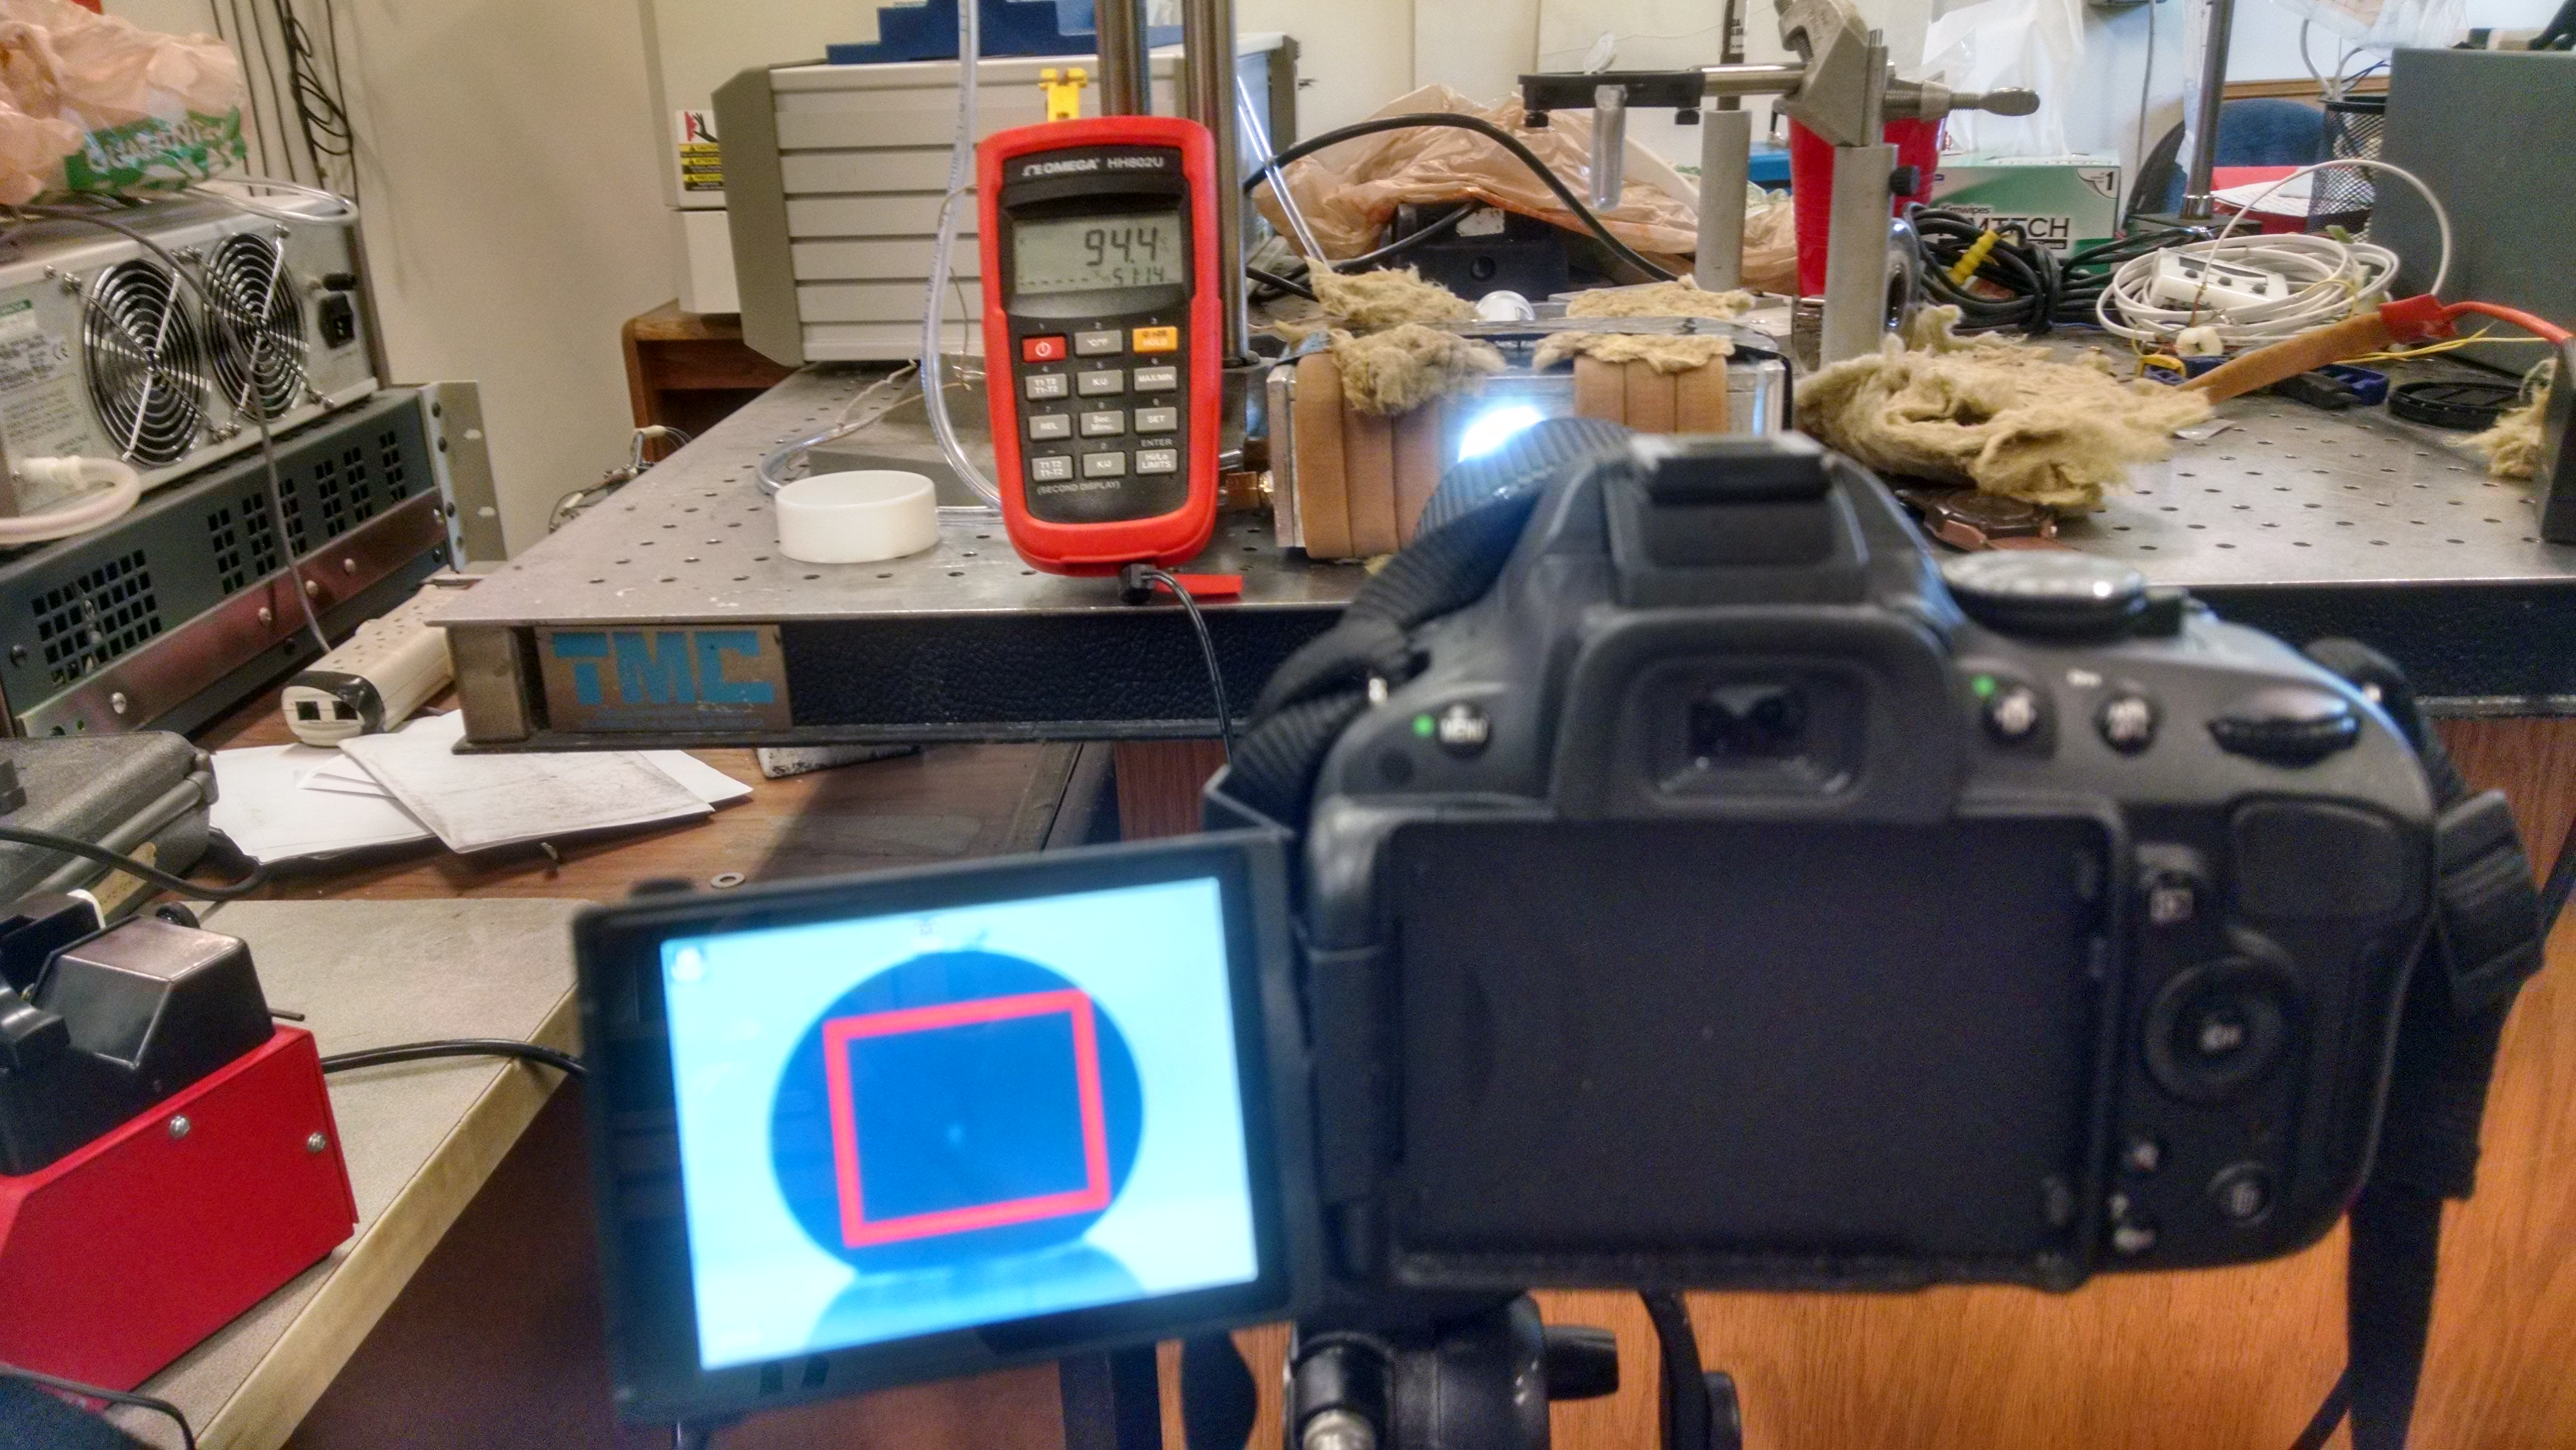
\includegraphics[width=\linewidth,trim={0 0 0 1cm}]{DSLRcamera}
	\caption{This is a photograph of a picture being taken of a gallium droplet on highly-textured polycrystalline at 94.4\degree C (seen from thermocouple meter) using a Nikon DSLR camera with a long macro-lens. }
	\label{fig:DSLRcamera}
\end{figure}

\subsection{Gallium Oxide removal}


While extensive steps have been taken to inhibit oxidation on the metal surfaces, preventing oxidation on the surface of liquid gallium was a greater challenge. Pure gallium and Gallium-based alloy surfaces very quickly oxidize in ambient air environments, and form turning a thin layer of gallium oxide (Ga$_{2}$O$_{3}$ and Ga$_{2}$O).\cite{Regan1995,Regan1997,Scharmann2004} Like any other metal, Ga has a high potential for spontaneous oxidation, or passivation. This oxide layer is solid and remains elastic until it experiences a yield stress. Therefore, that an oxidized gallium droplet does not behave as a simple liquid, but as a viscoelastic material. In addition, the oxide layer of gallium is known to adhere to almost any solid surface, causing a severe stiction problem that interferes with interfacial energy measurements.\cite{Scharmann2004}. This shows how dramatically the gallium surface tension decreases when the oxide forms. Khan \etal showed that gallium oxide forms hydroxyl groups on their exterior surface, making the drops lyophilic as opposed to the expected lyophobic behavior of pure gallium, a high surface tension liquid.\cite{Hardy1985,Alchagirov2005} 

\begin{figure}
	\centering
	\begin{subfigure}[c]{0.45\textwidth}
		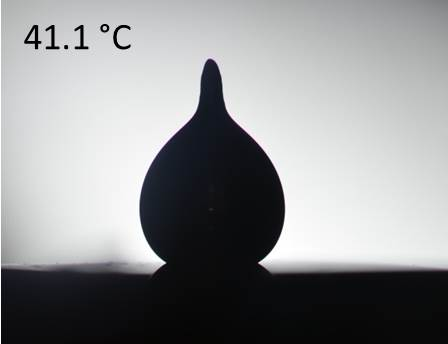
\includegraphics[width=\linewidth,trim={0 0 0 0}]{ga_41c}
		\subcaption{~}
		\label{fig:ga_41c}		
	\end{subfigure}
	\begin{subfigure}[c]{0.45\textwidth} 
		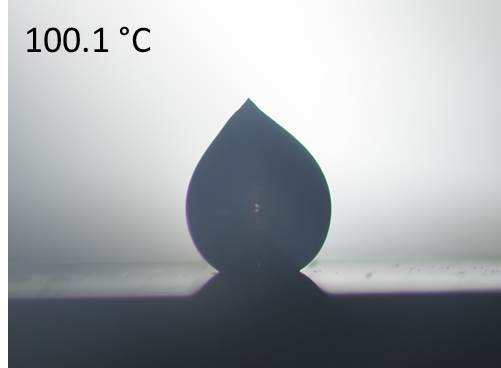
\includegraphics[width=\linewidth,trim={0 0 0 0}]{ga_100c}
		\subcaption{~}
		\label{fig:ga_100c}		
	\end{subfigure}
	\caption{Pure liquid gallium obtains viscoelastic properties when trace amounts of oxygen are present via formation of oxide shell. Non-axisymmetric Ga drops form on this iron substrate.}
	\label{fig:deformed_ga}
\end{figure}
Figure \ref{fig:deformed_ga} shows our direct observation of this phenomenon with teardrop shaped droplets formed by adhering to the iron surface while simultaneously being pulled upwards by the deposition needle. The general shape of these drops were unchanged for many hours even at temperatures approaching $\sim$100\degree C, thus exhibiting the stability of viscoelastic properties caused by the solid oxide layer. Removing the oxide layer from liquid gallium will return normal liquid properties to gallium and allow the use of axisymmetric drop analysis calculations: Young-Laplace equation, tangent method, and circle approximation method. 

Oxide removal permits liquid gallium to directly interact with metal surfaces instead of gallium oxide; the derived terms for \gamSL and \gamLV in Equation \ref{youngs-eqn-ga} become more robust. A number of techniques have been developed to remove and recover gallium oxide on liquid gallium: ultra-high vacuum (UHV) techniques,\cite{Regan1995,Regan1997} chemical vapor etching,\cite{Kim2013,Doudrick2014} and electrohydrodynamic phenomena.\cite{Khan2014} A chemical vapor etch is the best option for this experiment because it has a minimal effect on the surface of metals and the experimental apparatus does not need to be changed.  
To execute the vapor etch, a pendant drop of gallium was formed and a pipette of 37wt\% HCl was brought in close proximity to etch away the oxide layer. The same procedure was performed on the sessile drop of gallium on the desired surface to etch away any oxide left on top of the droplet, as seen in Figure \ref{fig:hcl_vapor_treat}. The contact angles of gallium on bare glass before and after HCl vapor treatment are similar to respective contact angle values in Kim \etal\cite{Kim2013}

The HCl vapor etch may even have the benefit of removing any native iron oxides (Fe$_2$O$_3$) from the FeGa surface itself since HCl is a known etchant of Fe$_2$O$_3$.\cite{Walker1991}



\begin{figure}
	\centering
	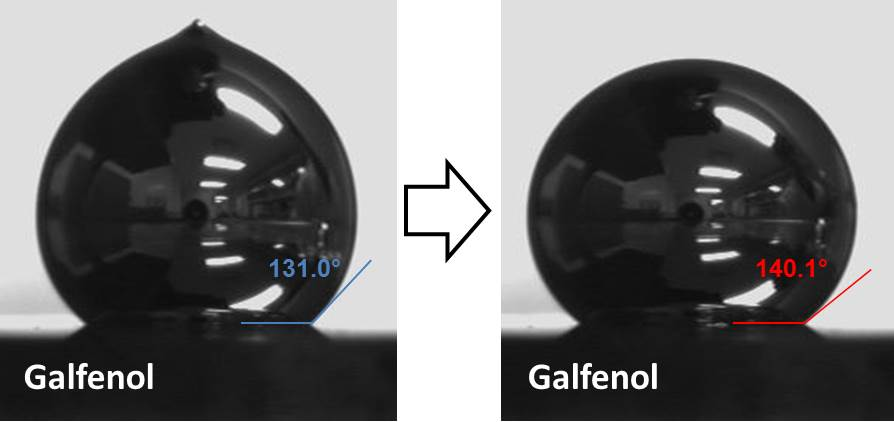
\includegraphics[width=\linewidth,trim={0 0 0 1cm}]{hcl_vapor_treat}
	\caption{This image shows the contact angle of gallium on a Galfenol sample in an argon environment before and after HCl vapor treatment.}
	\label{fig:hcl_vapor_treat}
\end{figure}







\section{Final experimental design and Results}\label{section2-3}

\subsubsection{Polycrystalline Metals}

With the HCl vapor treatment added to the procedure, temperature-varying gallium contact angle measurements in an argon environment were executed in the aluminum chamber on multiple metal substrates. Polycrystalline samples of high purity ($>$99.99\%) tin, copper, and iron were polished and had liquid gallium deposited on their surfaces. The temperature in the chamber was slowly ($<$10\degree C/min) increased from ~30\degree C to just below 100\degree C. Beyond 100\degree C, the heating tape becomes inconsistent with the intervals of heat applied to the chamber. Photographs of gallium drop profiles are taken at ~10\degree C intervals to observe progression of the drop shape as temperature increases. The same procedure is done as the temperature is decreased to 30\degree C to observe reversibility of this process, since we assume that the thermal expansion of the substrate drives the change in \gamSL from Equation \ref{youngs-eqn-ga}. 

A chemical vapor etch is used to replace the gallium oxide () layer with a gallium chloride layer, restoring the droplet surface tension to nearly that of pure Ga, as shown by Kim \etal To execute the vapor etch, a sessile drop of gallium was formed on the desired surface and a pipette of 37wt\% HCl was brought within 2 cm to etch away the gallium oxide layer. 

It is known that liquid gallium tends to corrode most metal surfaces.\cite{Lewandowski2015,Narh1998,Fitzgerald1999} Since experiments lasted for less than one hour, corrosion between the two metals should not be significant enough to effect the measurement. Later in this \hyperlink{xps-gallium}{section}, the surface stoichiometry effects of the liquid Ga droplet on Galfenol for varying temperatures is examined using X-ray photoelectron spectroscopy (XPS). For the polycrystalline tin and copper samples, gallium began to visibly corrode through the surface between 60\degree C and 70\degree C, as evident by a rapid contact angle decrease on only side of the drop profile, as seen in Figure \ref{fig:copper-tin-gallium-CA}. Polycrystalline iron samples did not experience corrosion problems throughout the experiments. It is expected that as the temperature increases, the thermal expansion of the solid will isotropically expand the drop thus decreasing the contact angle. Some gallium contact angles decrease on iron, but it is often that the decrease occurs on one side of the drop profile as the temperature increases. This is most likely due to the polycrystalline grains having different thermal expansions, hence the drop spreading is anisotropic. This suggests that a single-crystal grain or highly-textured surface grain is needed to properly observe an isotropic drop expansion. 
\begin{figure}
	\centering
	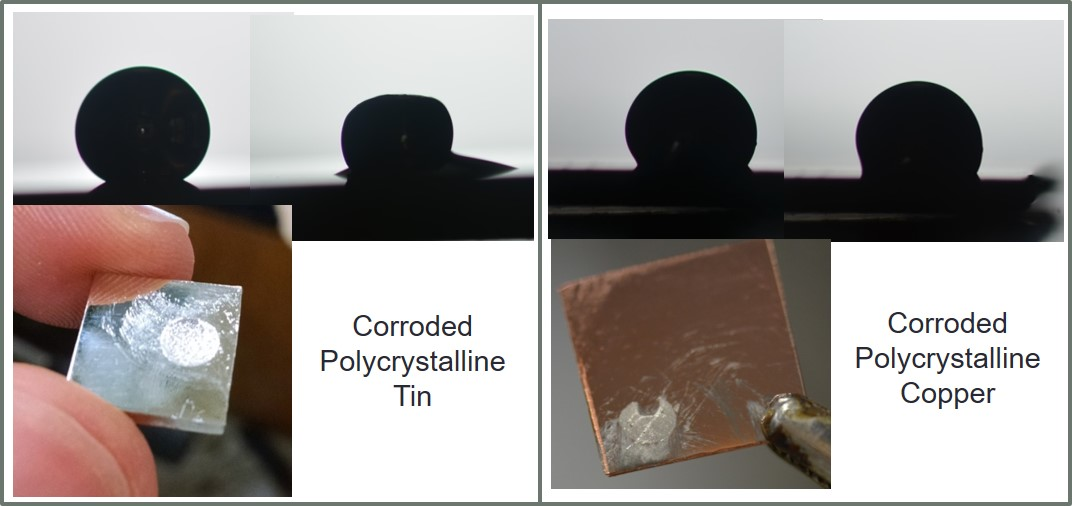
\includegraphics[width=\linewidth,trim={0 0 0 2cm}]{copper-tin-gallium-CA}
	\caption{These photographs show a gallium drop contact angle on polycrystalline Sn (left) and polycrystalline Cu (right), and the corrosive effects of the gallium on the same substrates.}
	\label{fig:copper-tin-gallium-CA}
\end{figure}



Since the iron sample did not corrode in the presence of gallium, we proceeded to a Galfenol sample with an abnormally grown \hkl(110) grain. Figure \ref{fig:ca_ebsd} shows the location of a gallium droplet in contact with the highly Goss-textured surface. Using the same temperature intervals, the right and left contact angles were measured and the surface energy
\begin{figure}
	\centering
	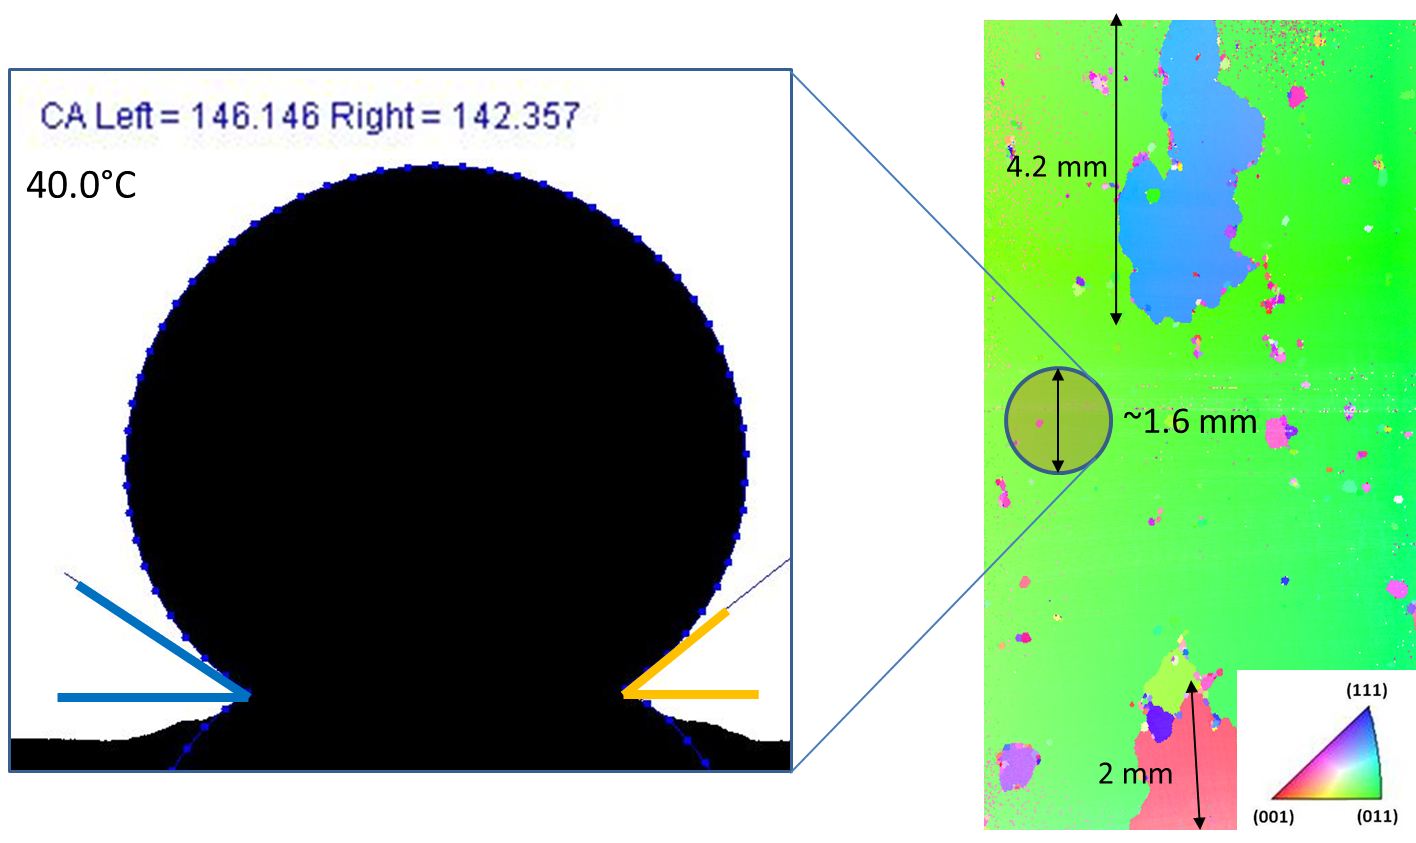
\includegraphics[width=\linewidth,trim={0 0 0 2cm}]{ca_ebsd}
	\caption{The location of a gallium drop on highly Goss-textured surface.}
	\label{fig:ca_ebsd}
\end{figure}
was calculated using Equation \ref{youngs-eqn-ga}. The contact angle measurements and surface energy calculations are shown in Figure \ref{fig:goss_se_msrmnt}. The contact angle measurements show anisotropic spreading behavior since the left contact angle recedes as temperature increases while the right contact angle advances. At 60.7\degree C, the contact angles reached close to the same value which may indicate an equilibrium point of combating thermal expansions caused by nearby island grains. 

Both right and left contact angles were measured at each temperature and used in Equation \ref{youngs-eqn-ga} to calculate the substrate surface energy. Plots of contact angle measurements and surface energy estimates are shown in Figure \ref{fig:goss_se_msrmnt}. The contact angle measurements show anisotropic spreading behavior since the left contact angle recedes as temperature increases while the right contact angle advances. Asymmetries may be associated with nearby island grains that are evident in the electron backscatter diffraction (EBSD) scan of Figure \ref{fig:ca_ebsd}. The magnitude of surface energy values in Figure \ref{fig:goss_ga_se} are on the order of 100 J/m$^2$ and the values increase as temperature increases. We had expected surface energy values to be closer in magnitude to DFT predicted values for $\alpha$-iron of $ \gamma_{SV}(T)$ = 2.0535 J/m$^2$, which has the same body-centered cubic crystal structure as Galfenol.\cite{Wang2000} We had also expected a decrease in surface energy with increasing temperature. This is because surface energy depends on the net inward cohesive force between atoms, and the cohesive force binding atoms to one another will decrease as a temperature increase causes atoms to vibrate more rapidly. We do not yet understand why the model leads to unexpected trends. We are currently examining the role of the $\gamma_{SL}(T)$ term in the model, as it is three orders of magnitude larger than the $\gamma_{SV}(T)$ term (due to the contribution from the Young's modulus value associated with Galfenol) and dominates the results.

\begin{figure}[h]
	\centering
	\begin{subfigure}[c]{0.47\textwidth}
		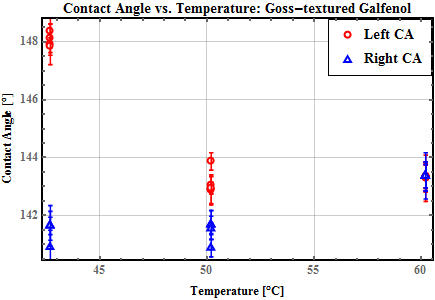
\includegraphics[width=\linewidth]{CAvsTemp_Goss-Galfenol3}
		\subcaption{~}
		\label{fig:goss_ga_ca}		
	\end{subfigure}
	\begin{subfigure}[c]{0.47\textwidth} 
		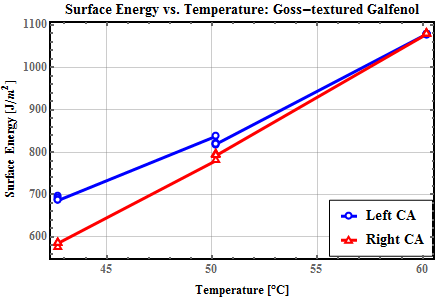
\includegraphics[width=\linewidth]{SEvsTemp_Goss-Galfenol3}
		\subcaption{~}
		\label{fig:goss_ga_se}		
	\end{subfigure}
	\caption{(a) Blue and red dots show left and right contact angle, respectively, of liquid gallium on \hkl(110) Fe-Ga. (b) Calculated surface energy values of \hkl(110) Fe-Ga grains using Equation \ref{youngs-eqn-ga}.}
	\label{fig:goss_se_msrmnt}
\end{figure}





\subsubsection{Single-crystal Galfenol}
Using the same acid vapor etch, Ga droplets were placed on samples of single crystal Galfenol. Contact angle values decrease from the (110), (100), and (111) facets (Figure 4), in that order, although the angles for the (100) and (111) facets are not statistically different (within one standard deviation of one another). According to Young’s equation, these contact angles should be inversely proportional to surface energy. The measurements indicate that the surface energy of a (110) surface has the lowest surface energy as expected based on DFT predictions.[5] The magnitudes of angles for (100) and (111) surfaces were statistically similar. Ga contact angles values on highly-textured Goss (110) grains and the (110) single crystal facet are within one standard deviation of one another, and thus in excellent agreement. 
%TODO insert single xtal figures here

\subsubsection{X-ray photoelectron spectroscopy study on Ga corrosion}

\hypertarget{xps-gallium}{XPS} measurements were performed after Ga drop experiments at the University of Maryland Surface Analysis Center using a high sensitivity Kratos AXIS 165 spectrometer to examine the effect of Ga droplets with a chloride shell affects the surface stoichiometry of Galfenol. Samples were prepared by placing a Ga drop on the Galfenol surface, heating the sample to a temperature of 30\degree C, 50\degree C ,70\degree C or 90\degree C, and holding that temperature for 15 minutes. The 70\degree C sample was damaged during XPS testing. XPS was also performed on a control sample that was not exposed to a Ga drop or elevated temperatures. 


XPS measurements show an increasing intensity in the Ga$_2$O$_3$ (1116.7 eV) peak in samples at elevated temperatures. This was expected as surface adhesion of Ga was likely greater in samples exposed to higher temperatures. Excess surface Ga would have oxidized in the time between the thermal tests and XPS due to exposure to ambient conditions. In the Fe region, a strong signal of Fe$_2$O$_3$ (710.8 eV) with a small peak of metallic Fe (706.7 eV) was present on the control sample. On the 30\degree C, 50\degree C and 90\degree C samples, the Fe$_2$O$_3$ peaks diminished and the metallic Fe peak became dominant. The increased presence of Ga at elevated temperatures suggests that the Ga may have etched away the Fe$_2$O$_3$ and exposed metallic Fe, as Ga is a corrosive element in the liquid state. The Ga signal is attributed solely to the Ga droplet as Fe has a higher potential for oxidation than Ga, shown by the heavy presence of Fe$_2$O$_3$ at the surface, and therefore Fe has a dominant concentration at the surface. 

%TODO insert figure of XPS measurements that show the above results. 
	
	

\section{Conclusions and next steps}\label{section2-4}
We have developed a new method for measuring the surface energy of targeted crystal orientations on metal surfaces. The model calculates surface energies on Goss-textured polycrystalline Galfenol and single crystal samples that are two orders of magnitude greater than theoretical predictions for $\alpha$-Fe. We have observed a qualitative trend in single crystal samples of different crystallographic orientations that matches predictions made using DFT simulations, where $\gamma_{100}$ and $\gamma_{111}$  are similar in magnitude ($<$5\% difference) and $\gamma_{110}$ is ~20\% less than values of $\gamma_{100}$ and $\gamma_{111}$. Future contact angle experiments will be performed strictly on single crystal samples due to greater uniformity of crystal orientations at the surface when compared to highly-textured rolled Galfenol sheets with multiple island grains at the surface. This uniformity will guarantee consistent interactions at the Ga-Galfenol-Ar triple line. The presence of a nanometer layer of Fe$_2$O$_3$ on Galfenol hinders this surface energy measurement. More thorough cleaning and polishing techniques, including chemical and plasma etches, in inert environments will be employed to eliminate or mitigate this layer formation. The model will be tested on large grains of oriented iron crystals and on well-characterized low energy surfaces (i.e. PTFE, etc.) with water as the probe liquid at temperatures below room temperature. We will revisit our derivation to address potential sources of error in magnitude. The interaction between the Ga and Galfenol interface is not well understood, and an in-situ measurement would need to be done to observe this reaction or lack thereof. Currently, this in-situ measurement is beyond current capabilities, so it is unknown how it would even affect the Ga contact angle measurement. Further investigation of this model and method offers potential for surface energy characterization of any metal with grain sizes $ > $2 mm to accommodate the minimum size of the probe droplet.

After presenting these preliminary findings at the XXIV International Materials Research Congress and 2015 MRS Fall Meeting,\cite{VanOrder2015a,VanOrder2015} I discussed possible avenues of improvement for the gallium contact angle experiment with colleagues and potential collaborators. A more concrete measurement of \gamSL between liquid gallium and solid would need to be examined, a very non-trivial task. Ultimately, we decided to suspend the gallium drop experiment and re-evaluate the measurement strategy. 
 %for obtaining orientation-dependent surface energies of magnetostrictive materials. 
 
Overall, this was an exploration of well-proposed and innovative research. Assumptions were made about how the system would interact and efforts to achieve good results in the lab were made. It was determined that these assumptions were too great and the experiment failed to meet expectations. Much was learned about the complexity of surface energy research from both a theoretical and experimental perspective. This failure persuaded me to find a more robust and promising method for accomplishing project goals within the constraints of orientation-dependent surface energy characterization. 

%TODO parse this section of article to LAtex code



\section{Metal Surface Energy Measurement}\label{section2}

\begin{outline}[enumerate]
\1 See MRS Advances paper
	
\end{outline}

%
The interactions of water with a low-energy and high-energy solid surface differ significantly. The relative energy of a solid compared to a liquid has to do with the bulk nature of the solid. Solids with weak molecular crystals (e.g., fluorocarbons, hydrocarbons, etc.) where the molecules are held together by weak physical forces (e.g., van der Waals and hydrogen bonds) are termed low-energy solids. A very low input of energy is required to break these solids, thus they typically have surface energy values $<$72 mJ/m$^2$.  Metals, glasses, and ceramics are known as "hard solids" because the chemical bonds that hold them together (e.g., covalent, ionic, or metallic) are very strong. Thus, these surfaces are high-energy because of the high amount of energy needed to break these solids to make two new surfaces, (e.g. see Equation \ref{SFE} in Section \ref{define-surf-energy}). High energy solids typically have surfaces energies $>$72 mJ/m$^2$.  The threshold between these two types of surfaces lies in their surface energy values relative to the surface tension of water, $\sim$72 mJ/m$^2$. Water tends to partially wet a low energy surface and completely wet a high energy surface based on how much lesser or greater the surface energy of the solid is compared to water, respectively. 

I will investigate two approaches to overcome the challenges involved in measuring the surface energy of metals using contact angle measurements. The first will study temperature variations of Galfenol surface energy using a droplet of gallium as the probe liquid. Gallium is a liquid with a surface tension at room temperature that is roughly one order of magnitude higher than that of water: $\gamma_{Ga}\sim$715.3 mJ/m$^2$. It is expected that a measurable contact angle will form between Galfenol and liquid gallium, and this information will be incorporated into an analytical model to extract the solid surface energy. The second will build on the two-liquid-phase technique to form a measurable water contact angle on the surface of Galfenol. To supplement this measurement, Galfenol samples will be patterned with a planned roughness to increase the water contact angle and properly determine the Young's contact angle to be used in surface energy calculations. Both experiments will use highly Goss textured Galfenol as well as single-crystal Galfenol samples to assure isotropic crystal orientation for contact angle measurements. 

Once experimental results are validated with published values, DFT predictions of the surface energy associated with different crystallographic orientations in Fe-Ga and Fe-Al will be tested and verified. This task and the resultant capability should have broad applicability beyond the needs of this proposal for extension to polycrystalline textured metals and thin films.
%This method has the potential to become a valuable tool for obtaining empirical surface energy data associated with AGG of Galfenol grains as well as other metallurgical studies.
%/research that lack experimental verification of surface energy around room temperature. 
%




\subsection{Phase I: Gallium Drop Method}


\begin{wrapfigure}[12]{R}{0.5\linewidth}
	\begin{subfigure}[b]{0.5\textwidth}
		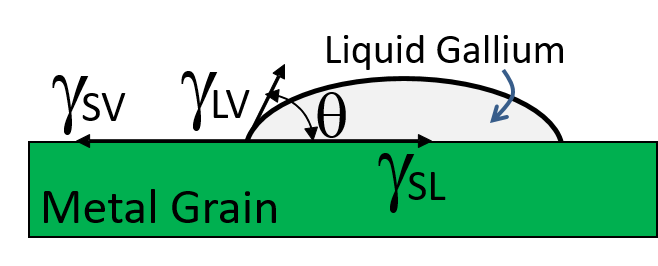
\includegraphics[width=\textwidth,trim={0 0 0 2cm}]{youngs-ga}
	%	\caption{Interfacial tensions on Ga drop on solid surface}
		\label{fig:youngs-ga}
	\end{subfigure}
	%add desired spacing between images, e. g. ~, \quad, \qquad, \hfill etc. 
	%(or a blank line to force the subfigure onto a new line)
	\begin{subfigure}[b]{0.5\textwidth}
		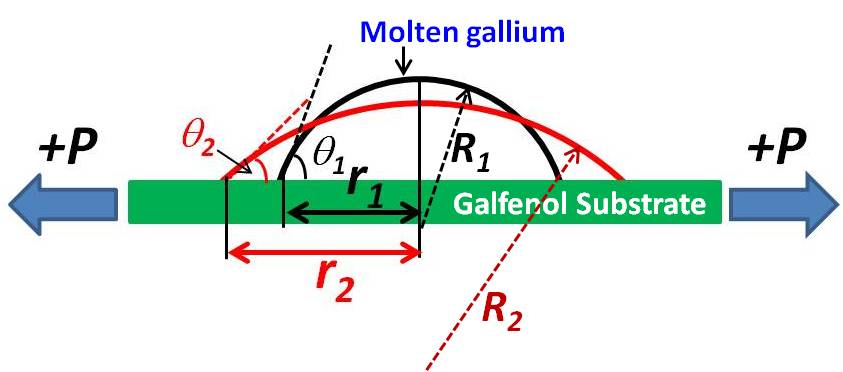
\includegraphics[width=\textwidth,trim={0 2cm 0 0}]{thermal-expand-drop}
	%	\caption{Thermal expansion of drop}
		\label{fig:thermal-expand-drop}
	\end{subfigure}
	\caption{Schematics indicating notation used and contact angles $\theta_{i}$, radii of drop-solid contact area $r_{i}$, and radii of curvature for a spherical drop $R_{i}$, for two temperatures as thermal expansion induced tension $P$ strains the substrate.}
	\label{fig:therm-exp-ga}
\end{wrapfigure}
The first technique employs measurement of contact angles and drop size of a liquid metal, gallium, resting on a metal surface as the metal is heated. Changes in surface tension will be introduced by controlled thermal expansion of the substrate at temperatures ranging from $\sim$30-100\degree C to give mobility to the molten gallium drop.
% and ensure that surface heterogeneities do not obscure the drop-substrate contact angle. 
A video system will be used to precisely quantify dimension changes in substrate and liquid metal drop during thermal expansion will be used. The surface energy of the free surface of the substrate as a function of temperature, $\gamma_{SV}(T)$, can be related to thermal-expansion-induced changes in the liquid gallium drop contact angle $\theta$, the radius $r$ of the liquid gallium drop in contact with the metal surface, and the height $h$ of the hemisphere of liquid gallium. 

These can be modeled as a tensile load +$P(T)$ caused by substrate thermal expansion (Figure \ref{fig:therm-exp-ga}), which effectively appears as a uniform radial expansion of the planar solid surface as temperature increases. By letting the system equilibrate at different temperatures before measuring liquid drop geometry, terms due to variation in thermal energy and variation of the total Gibbs free energy vanish. Then, the interface energy between the substrate solid and the liquid gallium drop, \gamSL, is given as \gamSL$=P(T)/2\pi r$. The uniform tension introduced by thermal expansion of substrate can be expressed as:
\begin{equation}\label{uniform-tension}
	P(T) = E_{sub}\alpha_{sub}(T-T_{mp})
\end{equation}
where $T_{mp}$ is the melting temperature of gallium, $E$  is the substrate Young’s modulus, and $\alpha$ is the linear thermal expansion coefficient. A linear function can be used to write the gallium-air interfacial tension a function of temperature, \gamLV $= a-b(T-T_{mp})$, where \textit{a} and \textit{b} are positive constants found experimentally.\cite{Hardy1985,Alchagirov2005} Putting the terms for \gamSL and \gamSV into \hyperlink{youngeqn}{Young’s equation}\cite{Rudawska2009,Tadmor2004}:
\begin{equation*}%\label{youngs-eqn-ga1}
	\gamma_{SV} =  \frac{E_{sub}\alpha_{sub}(T-T_{mp})}{2\pi r} + \left[a-b(T-T_{mp})\right]\cos\theta
\end{equation*}

A relationship between the variable radius $r(T)$ associated with the area of the circular region of solid-liquid contact $A_{SL}(T)$, the contact angle $\theta(T)$ and the volume $V$ of the spherical cap formed by the drop is derived next. To determine the radius $r(T)$, the geometric relationships based on the radius of curvature $R(T)$ of a sphere is mapped onto the hemispherical liquid cap. The drop is modeled as being part of a sphere whose radius is $R(T)$. It is assumed that he volume $V$ of the drop is the volume of the spherical cap, and remains constant. The radius $R(T)$ can then be expressed in terms of the volume and the angle:
\begin{equation*}\label{drop-geom}
	R(T) = V^{1/3} \left[\frac{\pi}{3} \left(2-3\cos\theta(T)+\cos^{3}\theta(T)\right)\right]^{-1/3}
\end{equation*}
Using the relation $r(T)=R(T)\sin\theta(T)$ (i.e. $\theta=$0\degree corresponds to complete wetting of the surface and at $\theta=90$\degree,  $r=R$) the following formula for surface energy as a function of temperature $T$ and contact angle $\theta(T)$ (shown as $\theta_{T}$) is:
\begin{equation}\label{youngs-eqn-ga}
	\gamma_{SV} =  \underbracket{\frac{E_{sub}\alpha_{sub}(T-T_{mp})}{2\pi}\left[\frac{\pi\left(2-3\cos\theta_{T}+\cos^{3}\theta_{T}\right)}{3V\sin^{3}\theta_{T}} \right]^{1/3}}_{\text{\gamSL(T)}} + \underbracket{\left[a-b(T-T_{mp})\right]}_{\text{\gamLV(T)}} \cos\theta_{T}
\end{equation}
This gives the surface energy \gamSV of specific grains as a function of temperature by measuring $T$ and $\theta$ at thermal equilibrium.

One of the challenges in developing this new surface energy measurement capability is the need to expose the surface of the metal substrate that is shielded by surface oxides. The following strategies for removing the oxide layer and preventing  natural oxidation, thereby increasing the accuracy of measurement, will be employed independently and in combination:
\begin{outline}
	\1 A flux used in high-temperature metal joining processes plays roles of dissolving of the oxides on the metal surface and preventing of re-oxidation as a chemical agent.
	\1 Colloidal silica polishing with nano-sized particles, such as is used for precise surface observations, like EBSD scans, which require clean surfaces to accurately detect patterns.
	\1 Electro-polishing is effective for passivation of clean surfaces after chemical and mechanical polishing for removal of surface oxides. 
\end{outline}
%Results using the proposed approach were to be validated through comparison of results for oriented single crystals with published theoretical values for pure metal elements of a specific crystallography (e.g. Ni, Cu, Fe)  and comparison with experimental data from amorphous metals (e.g. Vitreloy or liquid steel) with destructive high temperature methods for measuring surface energy. 
It should be noted that all of these techniques will not prevent oxides from forming for an extended period of time. Therefore, the cleaning would have to be followed by isolation in high vacuum, an inert environment, or another liquid environment that prevents oxidation.







%todo: Go through each version, and mark what was improved upon from experimental progression. 

\subsubsection{Contact Angle Goniometer (Verison 1)}
Preliminary designs of my contact angle goniometer implement a radiative temperature control box which encloses an argon gas filled container where the sample resides, as seen in Figure \ref{fig:rad-temp-box}.  The presence of argon is meant to prevent any further oxidation of the Galfenol sample as well as the gallium droplet. The container was initially made of a clear acrylic plastic, but prolonged exposure to temperatures above 80\degree C caused thermal deformation of the plastic making longer experiments impossible to perform without environment contamination.  A clear pyrex container replaced the acrylic box to fix this issue.  Application of the liquid gallium drop to our surfaces was done via a mounted plastic syringe with disposable stainless steel hypodermic needles that were available at the time. Liquid gallium tends to adhere strongly to the stainless steel needle tips which makes wetting to the sample very difficult. The stainless steel tip tends to deform the highly viscous gallium drop resulting in non-uniform hemispheric drop shapes, as shown in Figure \ref{fig:deformed-ga}.
\begin{figure}[h]
	\centering
	\begin{subfigure}[c]{0.45\textwidth}
		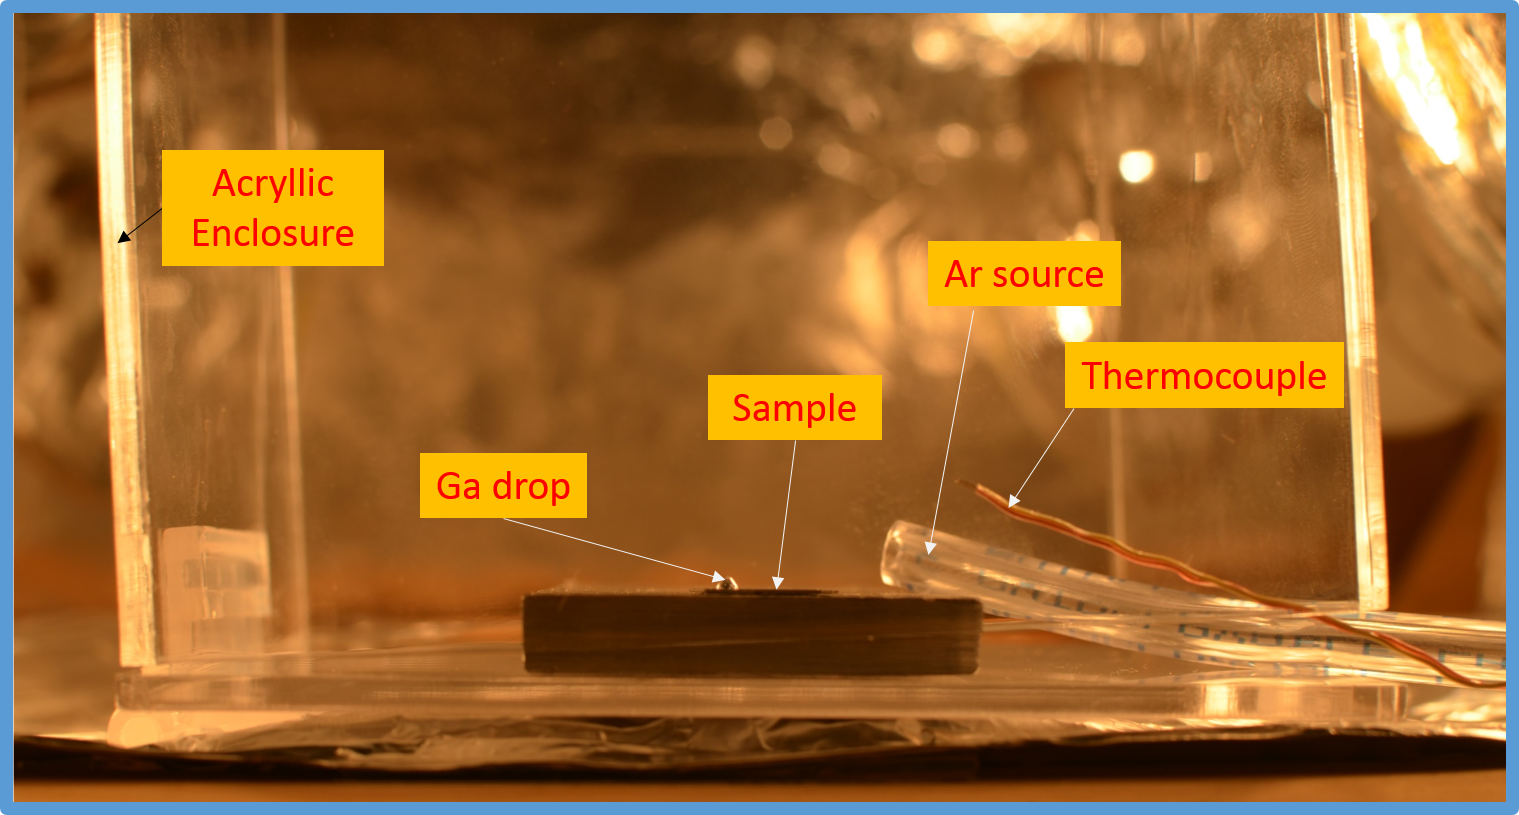
\includegraphics[width=\linewidth]{rad-temp-box}
		\subcaption{~}
		\label{fig:rad-temp-box}		
	\end{subfigure}
	\begin{subfigure}[c]{0.45\textwidth} 
		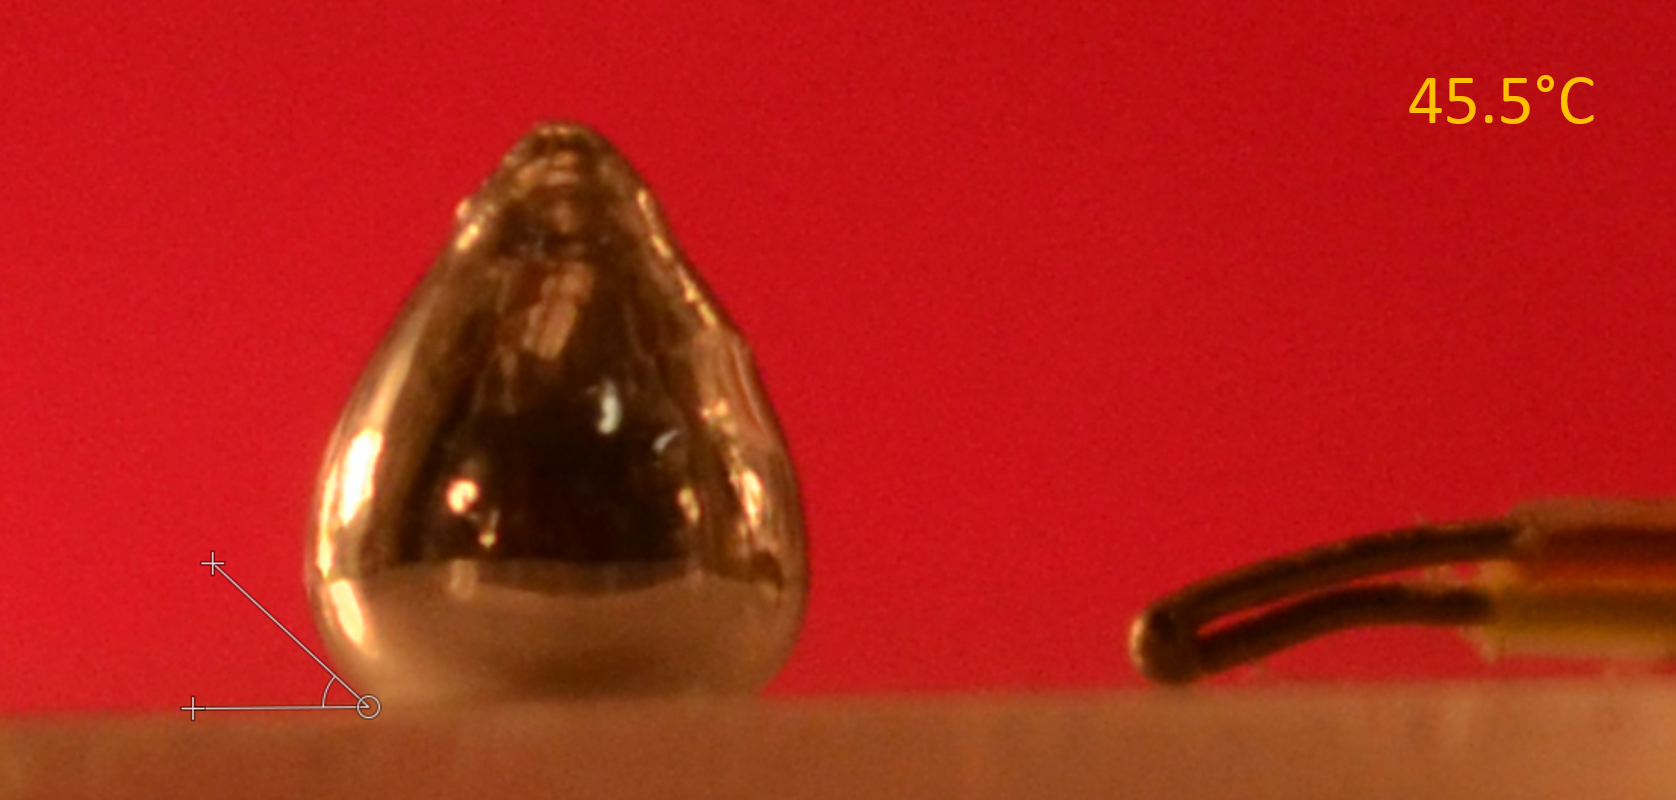
\includegraphics[width=\linewidth]{deformed-ga}
		\subcaption{~}
		\label{fig:deformed-ga}		
	\end{subfigure}
	\caption{(a) The first design of our contact angle goniometer.  The acrylic container houses the argon environment and sample.  This design was modified with a more stable glass enclosure. (b) A highly deformed gallium drop next to the thermocouple on a ceramic YAG test sample at 45.5\degree C.}
	\label{fig:prelim-design}
\end{figure}

For this experiment to succeed, a number of challenges were overcome. The simplest task involved polishing Galfenol samples using incrementally higher grit SiC paper and subsequent 0.1 $\mu$m colloidal silica particles to decrease the roughness to below 40 nm, as proven using AFM measurements. %TODO: Find AFM roughness picture?
% AFM roughness pic
%\begin{figure}
%	\centering
%		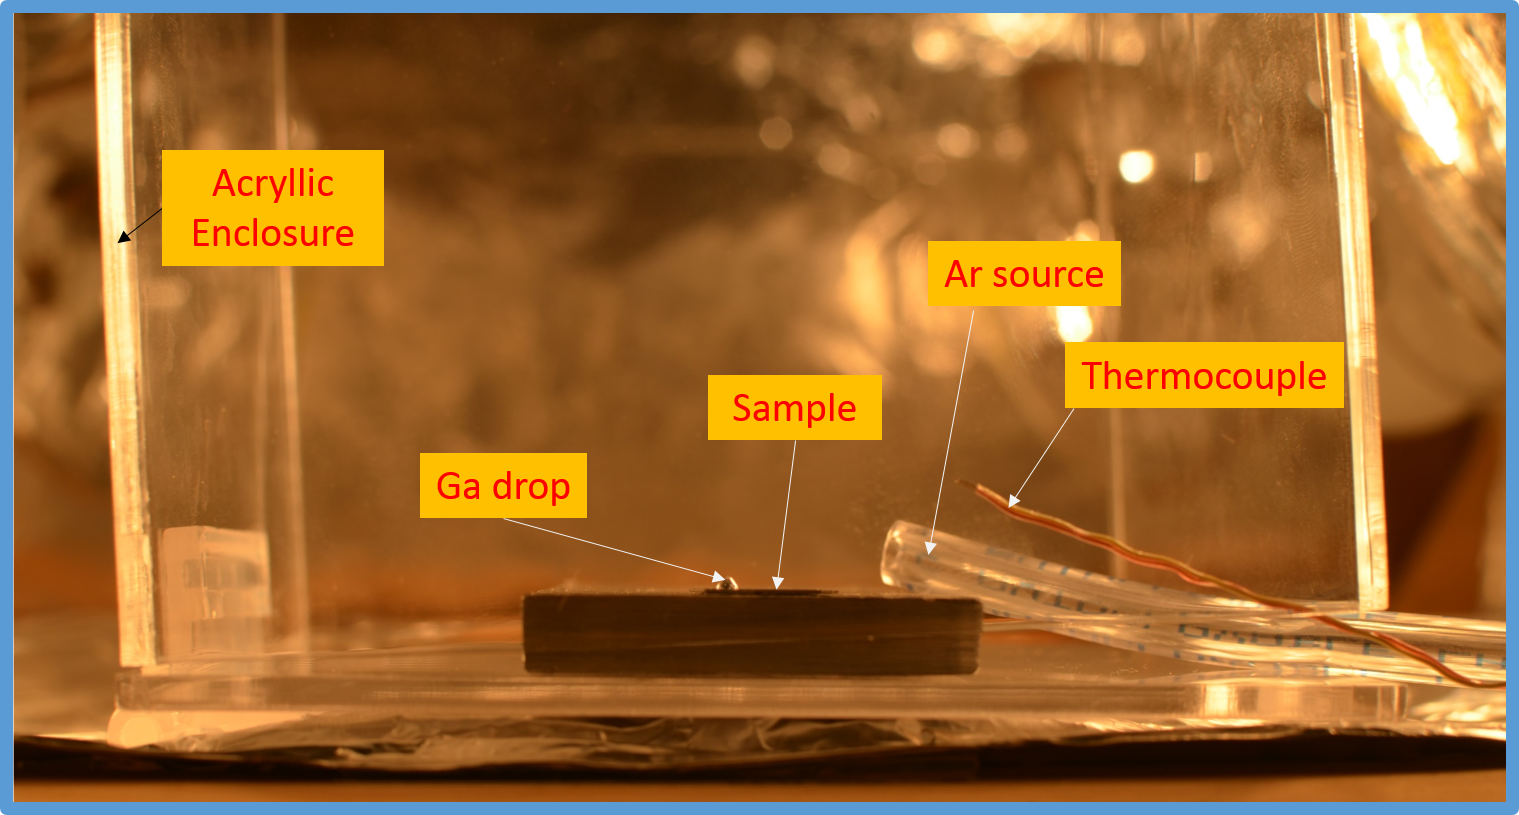
\includegraphics[width=\linewidth]{rad-temp-box}
%	\caption{(a) The first design of our contact angle goniometer.  The acrylic container houses the argon environment and sample.  This design was modified with a more stable glass enclosure. (b) A highly deformed gallium drop next to the thermocouple on a ceramic YAG test sample at 45.5\degree C.}
%	\label{fig:prelim-design}
%\end{figure}
The radiative box that housed this experiment had a high variability in temperature according to thermocouple readings, so a smaller apparatus with a top-side syringe opening is made to properly perform gallium drop tests at specific temperatures and prevent interaction with the experiment environment. There must also be bright white backlighting to obtain a high contrast drop profile. In this radiative box configuration, the high-reflecting liquid metal surface prevents a high contrast drop profile image, as seen in Figure \ref{fig:deformed-ga}. Proper contact angle measurements also require the gallium droplets to carefully wet the surface while forming an axisymmetric and spherical-like shape on the solid surface. A height adjustment system must be used to move the gallium pendant drop close enough to the sample surface for solid adhesive forces to overcome the adhesion to the needle. Lastly, the argon gas environment could be more well contained, instead of just filling up the glass sample enclosure from the bottom and spilling out the top due to higher density argon displacing the surrounding air environment. 

\subsubsection{Version 2}
\begin{figure}
	\centering
	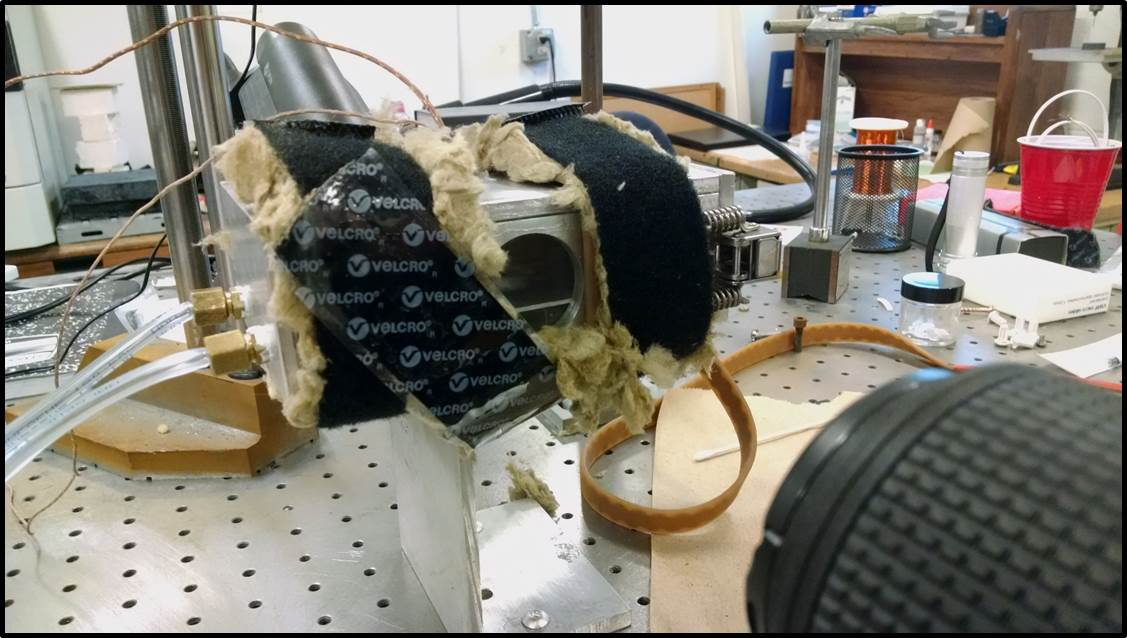
\includegraphics[width=\linewidth,trim={0 0 0 1cm}]{enviro_chamber}
	\caption{The second version of our gallium contact angle goniometer. The aluminum enclosure conductively transfers heat, the gas lines flow Ar gas into the chamber, top-mounted thermocouples monitor the gas and sample temperature, and the glass windows allow for backlighting of the drop profile along with high resolution image capture using a DSLR camera.}
	\label{fig:enviro_chamber}
\end{figure}
The new experimental apparatus can be seen in Figure \ref{fig:enviro_chamber}. The main structure is made of aluminum with two round glass windows on the front and back. The aluminum is meant to conductively transfer heat to the substrate by means of a heating cable wrapped around the outside of the structure. The high thermal conductivity of aluminum allows for a quick transfer of heat, thus an increased control of sample temperature. The time percentage dial controller attached to the heating tape is calibrated with the sample temperature using a thermocouple placed on the sample surface. Sample temperature can be consistently controlled with $\pm$0.5\degree C accuracy. Backlighting greatly improved the drop profile contrast by having only one white light source coming from one side of the droplet, as seen in Figure \ref{fig:deformed_ga}. The Ar environment is also far more contained and controlled. The silicone sealant creates a nearly air-tight system where the argon will displace all gas contaminants that could oxidize the sample or gallium droplet. 
%These precautions are suitable for any metals samples tested because each sample is polished according to the procedure described above and then cleaned with acetone to remove any oxides. 
Once the sample is inserted and sealed in the environmental chamber, the Ar prevents oxidation throughout the experiment. 
%A positive partial pressure is achieved in the chamber with an in- and out-valve. %TODO find more sufficient answer to how this removes oxides. 

While extensive steps have been taken to inhibit oxidation on the metal surfaces, preventing oxidation on the surface of liquid gallium was a greater challenge. Pure gallium and Gallium-based alloy surfaces instantly oxidize in ambient environments, turning into a thin layer of gallium oxide (Ga$_{2}$O$_{3}$ and Ga$_{2}$O).\cite{Regan1995,Regan1997,Scharmann2004} This oxide layer is solid and remains elastic until it experiences a yield stress. Therefore, that an oxidized gallium droplet does not behave as a simple liquid, but as a viscoelastic material. In addition, the oxide layer of gallium is known to adhere to almost any solid surface, causing a severe stiction problem that interferes with interfacial energy measurements.\cite{Scharmann2004}. This shows how dramatically the gallium surface tension decreases when the oxide forms. Khan \etal showed that gallium oxide forms hydroxyl groups on their exterior surface, making the drops lyophilic as opposed to the expected lyophobic behavior of pure gallium, a high surface tension liquid.\cite{Hardy1985,Alchagirov2005} 

\begin{figure}
	\centering
	\begin{subfigure}[c]{0.45\textwidth}
		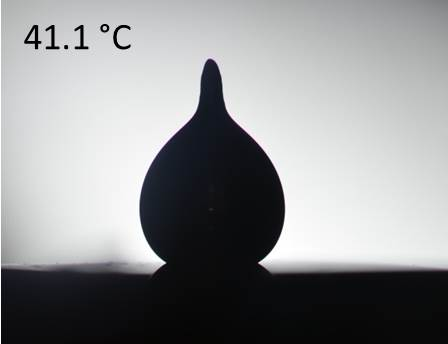
\includegraphics[width=\linewidth,trim={0 0 0 0}]{ga_41c}
		\subcaption{~}
		\label{fig:ga_41c}		
	\end{subfigure}
	\begin{subfigure}[c]{0.45\textwidth} 
		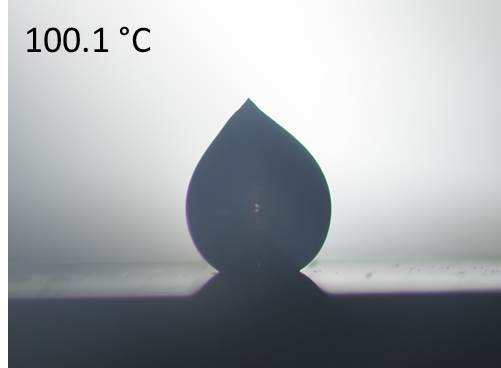
\includegraphics[width=\linewidth,trim={0 0 0 0}]{ga_100c}
		\subcaption{~}
		\label{fig:ga_100c}		
	\end{subfigure}
	\caption{Pure liquid gallium obtains viscoelastic properties when trace amounts of oxygen are present via formation of oxide shell. Non-axisymmetric Ga drops form on this iron substrate.}
	\label{fig:deformed_ga}
\end{figure}
Figure \ref{fig:deformed_ga} shows our direct observation of this phenomenon with teardrop shaped droplets formed by adhering to the iron surface while still being pulled upwards by the deposition needles. The general shape of these drops were unchanged for many hours even at temperatures approaching $\sim$100\degree C, thus exhibiting the stability of viscoelastic properties caused by the solid oxide layer. Removing the oxide layer from liquid gallium will return normal liquid properties to gallium and allow the use of axisymmetric drop analysis calculations: Young-Laplace equation, 
%todo: [NEED MORE TECHNIQUES FROM KRUSS GONIOMETER]



Oxide removal permits liquid gallium to directly interact with metal surfaces instead of gallium oxide; the derived terms for \gamSL and \gamLV in Equation \ref{youngs-eqn-ga} become more robust. A number of techniques have been developed to remove and recover gallium oxide on liquid gallium: ultra-high vacuum (UHV) techniques,\cite{Regan1995,Regan1997} chemical vapor etching,\cite{Kim2013,Doudrick2014} and electrohydrodynamic phenomena.\cite{Khan2014} A chemical vapor etch is the best option for this experiment because it has a minimal effect on the surface of metals and the experimental apparatus does not need to be changed. To execute the vapor etch, a pendant drop of gallium was formed and a pipette of 37wt\% HCl was brought in close proximity to etch away the oxide layer. The same procedure was performed on the sessile drop of gallium on the desired surface to etch away any oxide left on top of the droplet, as seen in Figure \ref{fig:hcl_vapor_treat}. The contact angles of gallium on bare glass before and after HCl vapor treatment are similar to respective contact angle values in Kim \etal\cite{Kim2013}

\begin{figure}
	\centering
	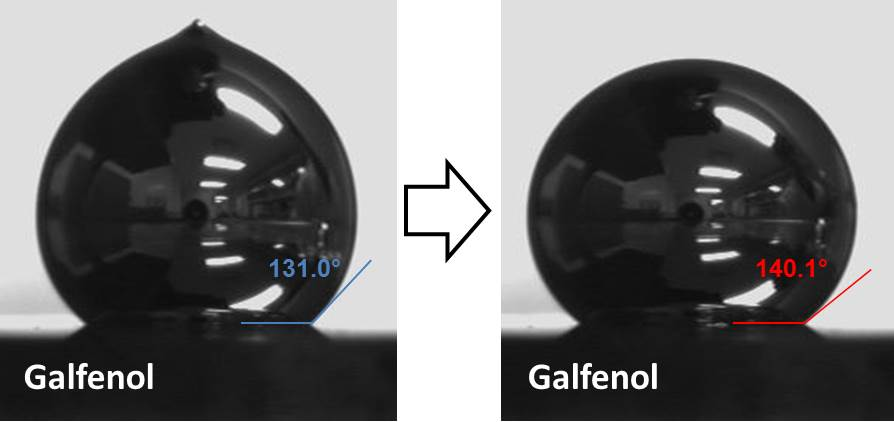
\includegraphics[width=\linewidth,trim={0 0 0 1cm}]{hcl_vapor_treat}
	\caption{This image shows the contact angle of gallium on a Galfenol sample in an argon environment before and after HCl vapor treatment.}
	\label{fig:hcl_vapor_treat}
\end{figure}

With the HCl vapor treatment added to the procedure, temperature-varying gallium contact angle measurements in an argon environment were executed in the aluminum chamber on multiple metal substrates. Polycrystalline samples of high purity ($>$99.99\%) tin, copper, and iron were polished and had liquid gallium deposited on their surfaces. The temperature in the chamber was slowly ($<$10\degree C/min) increased from ~30\degree C to just below 100\degree C. Beyond 100\degree C, the heating tape becomes inconsistent with the intervals of heat applied to the chamber. Photographs of gallium drop profiles are taken at ~10\degree C intervals to observe progression of the drop shape as temperature increases. The same procedure is done as the temperature is decreased to 30\degree C to observe reversibility of this process, since we assume that the thermal expansion of the substrate drives the change in \gamSL from Equation \ref{youngs-eqn-ga}. 

It is known that liquid gallium tends to corrode most metal surfaces.\cite{Lewandowski2015,Narh1998,Fitzgerald1999} Since experiments lasted for less than one hour, corrosion between the two metals should not be significant enough to effect the measurement. For the polycrystalline tin and copper samples, gallium began to visibly corrode through the surface between 60\degree C and 70\degree C, as evident by a rapid contact angle decrease on only side of the drop profile. Polycrystalline iron samples did not experience corrosion problems throughout the experiments. It is expected that as the temperature increases, the thermal expansion of the solid will isotropically expand the drop thus decreasing the contact angle. Some gallium contact angles decrease on iron, but it is often that the decrease occurs on one side of the drop profile as the temperature increases. This is most likely due to the polycrystalline grains having different thermal expansions, hence the drop spreading is anisotropic. This suggests that a single-crystal grain or highly-textured surface grain is needed to properly observe an isotropic drop expansion. 


Since the iron sample did not corrode in the presence of gallium, we proceeded to a Galfenol sample with an abnormally grown \hkl(110) grain. Figure \ref{fig:ca_ebsd} shows the location of a gallium droplet in contact with the highly Goss-textured surface. Using the same temperature intervals, the right and left contact angles were measured and the surface energy
\begin{figure}
	\centering
	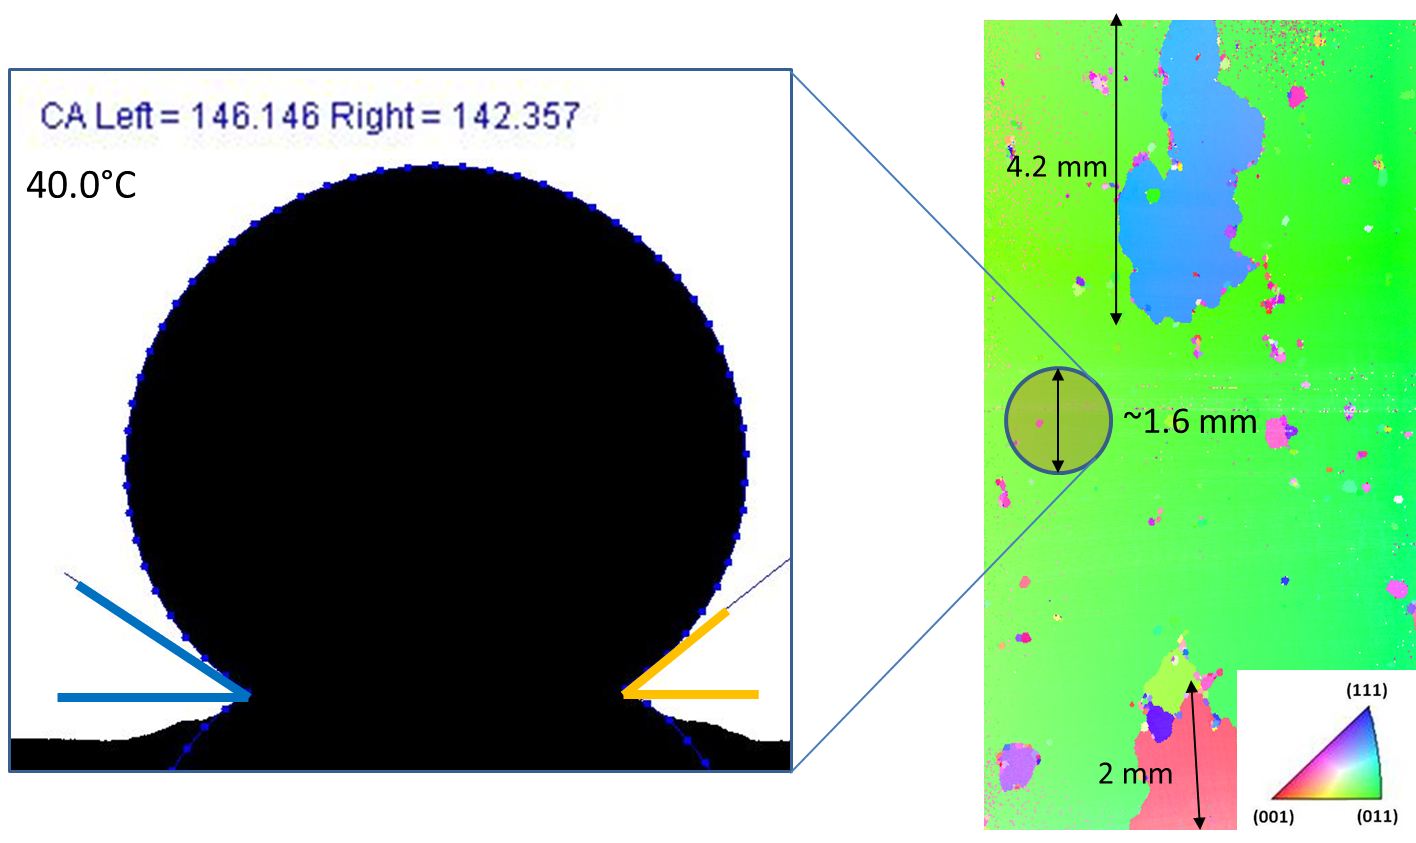
\includegraphics[width=\linewidth,trim={0 0 0 2cm}]{ca_ebsd}
	\caption{The location of a gallium drop on highly Goss-textured surface.}
	\label{fig:ca_ebsd}
\end{figure}
 was calculated using Equation \ref{youngs-eqn-ga}. The contact angle measurements and surface energy calculations are shown in Figure \ref{fig:goss_se_msrmnt}. The contact angle measurements show anisotropic spreading behavior since the left contact angle recedes as temperature increases while the right contact angle advances. At 60.7\degree C, the contact angles reached close to the same value which may indicate an equilibrium point of combating thermal expansions caused by nearby island grains. 

 The increasing surface energy trend as the temperature increased was not an expected result. As the temperature of a metal surface increases, the cohesive force binding atoms will decrease because the atoms will vibrate more rapidly. Since surface energy depends on the net inward cohesive force, a decrease in surface energy with increasing temperature was expected. Moreover, such a high difference in surface energy as the temperature increased was not expected. The $ \gamma_{SL}(T) $ term is extremely dominant compared to the $ \gamma_{LV}(T) $ term. This is due to the high Young's modulus value associated with Galfenol. The values of surface energy for the \hkl(110) Galfenol grain are two orders of magnitude greater than predicted values of $\alpha$-iron, \gamSV = 2.0535 J/m$^2$.\cite{Wang2000} 
\begin{figure}[h]
	\centering
	\begin{subfigure}[c]{0.47\textwidth}
		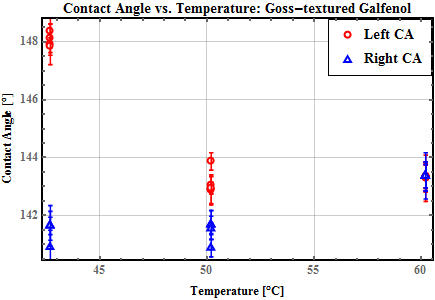
\includegraphics[width=\linewidth]{CAvsTemp_Goss-Galfenol3}
		\subcaption{~}
		\label{fig:goss_ga_ca}		
	\end{subfigure}
	\begin{subfigure}[c]{0.47\textwidth} 
		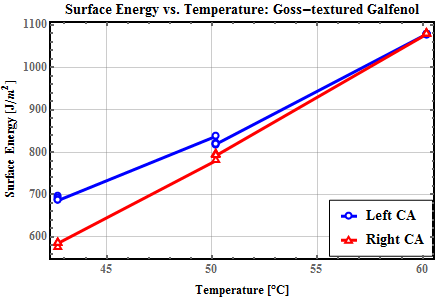
\includegraphics[width=\linewidth]{SEvsTemp_Goss-Galfenol3}
		\subcaption{~}
		\label{fig:goss_ga_se}		
	\end{subfigure}
	\caption{(a) Blue and red dots show left and right contact angle, respectively, of liquid gallium on \hkl(110) Fe-Ga. (b) Calculated surface energy values of \hkl(110) Fe-Ga grains using Equation \ref{youngs-eqn-ga}.}
	\label{fig:goss_se_msrmnt}
\end{figure}
 After presenting these preliminary findings at the XXIV International Materials Research Congress and 2015 MRS Fall Meeting,\cite{VanOrder2015a,VanOrder2015} I discussed possible avenues of improvement for the gallium contact angle experiment with colleagues and potential collaborators. A more concrete measurement of \gamSL between liquid gallium and solid would need to be examined, a very non-trivial task. Ultimately, we decided to suspend the gallium drop experiment and re-evaluate the measurement strategy. 
 %for obtaining orientation-dependent surface energies of magnetostrictive materials. 
 
Overall, this was an exploration of well-proposed and innovative research. Assumptions were made about how the system would interact and efforts to achieve good results in the lab were made. It was determined that these assumptions were too great and the experiment failed to meet expectations. Much was learned about the complexity of surface energy research from both a theoretical and experimental perspective. This failure persuaded me to find a more robust and promising method for accomplishing project goals within the constraints of orientation-dependent surface energy characterization. 
%TODO: don't say failure in the last sentence. Find a different way to build yourself up.




%\subsection{Results and Presentations}

%TODO: Explain why this method is not possible from a fundamental thermodynamic position (ie using one thermodynamic equilibirum and plugging it in to another equation at thermodynamic equilibrium). Should be able to go from one thermodynamic equilibrium equation to another, but that is not the case here. The method could still be feasible if more terms (\gamSL between liquid-Ga and solid) were known



\chapter{Patterned Two-Liquid-Phase Method}\label{chapter3}

\begin{outline}[enumerate]
\1 Schultz Method (Two-liquid-phase method)
	\2 Experimental Apparatus
\1 Nearly-flat surface results
	\2 Polishing procedure to remove oxide layer
		\3 Polishing and cleaning options at UMD
			\4 XPS results + quantitative analysis
		\3 Polishing at NSWC Carderock
	\2 Results for Carderock polished single crystal samples
		\3 Retained presence of iron oxide
	\2 Dry polish results (Week of Jan 2nd)
	
	\2 Plasma sputtered result (Week of Jan 9)
		\3 Using sputterer in Phaneuf glovebox
		
\1 Patterned surface results
	\2 Learn to use sputterer in Phaneuf glovebox?
	\2 Learn to do spin-coating from FabLab
		\3 Thick photoresist using A2 4620 (suggested by FabLab), which can get a 14 $\mu$m thick layer
	\2 Perform dry etch and spin coating in Phaneuf glovebox
	\2 Do UV processing somewhere
		\3 FabLab?
	\2 Use Ion mill for etching by scheduling with Xiaohang on Google Calendar
		\3 Ask for one more demo with him supervising. 
	
\1 Force curve measurement
	
	
	
\end{outline}


\subsection{Phase II: Two-liquid-phase contact angle method}

The next method returns to the idea of water contact angles on metal surfaces. As described previously, water will spread completely on a nearly-flat metal surface surrounded by a gaseous environment. Instead of a gaseous environment, the water-metal system can be surrounded by another liquid. It has been observed that instead of wetting completely, a water droplet will only partially wet a metal when the surrounding environment is an immiscible liquid. This is called the two-liquid-phase contact angle method developed by Jacques Schultz.\cite{Schultz1977,Schultz1977a,Schultz1992} 


A full derivation of this method can be found in Appendix \ref{appendixB}. In order to calculate the dispersive component of \gamSV for a solid surface, the water \ca must be measured on a solid immersed in \nalk[s]. By interpreting Equation \ref{schultz2} as a classic linear function, $y = mx + b$:

\[
\underbracket{\gamma_{W}-\gamma_{H}+\gamma_{WH}\cos\theta_{W}}_{\text{\normalsize{$y$}}} =
\underbracket{2(\gamma_{S}^{D})^{1/2}}_{\text{\normalsize{$m$}}}  
\underbracket{[(\gamma_{W}^{D})^{1/2}-(\gamma_{H}^{D})^{1/2}] }_{\text{\normalsize{$x$}}} + 
\underbracket{I_{SW}^{P}}_{\text{\normalsize{$b$}}} 
\] 
$\gamma_{W}$, $\gamma_{H}$, and $\gamma_{WH}$ are known from consistently confirmed literature values,\cite{Chassin1986,Smitthipong2004,Takanashi2013,Nakamura2015} and are listed in Table \ref{knownsurften}. A data set of \textit{xy}-coordinates will be made by dropping water in an \nalk environment to determine $\gamma_{S}^{D}$ and $I_{SW}^{P} $. $\gamma_{S}^{D} $ will be calculated from the slope of the measured dataset. 

\begin{table}[h!]
	\centering
	\caption{Hydrocarbon surface tension and water-hydrocarbon interfacial energy}
	\begin{tabular} { |c||c|c|  } %\label{nalkSE}
		%	\hline
		%	\multicolumn{3}{|c|}{Hydrocarbon surface tension and water-hydrocarbon interfacial energy}\\
		\hline
		\textbf{\nalk[s]}	&\textbf{$\bm{\gamma_{H}}$ (mJ/m$\bm{^{2}}$)}	&\textbf{$\bm{\gamma_{WH}}$ (mJ/m$\bm{^{2}}$)}	\\
		\hline
		hexane		&18.4	&50.1 \\
		\hline
		octane		&21.7	&49.8 \\
		\hline
		decane		&23.8	&51.0 \\
		\hline
		hexadecane	&27.5	&51.3 \\
		\hline
	\end{tabular}
	\label{knownsurften}
\end{table}

%TODO: define London 

The polar component of the solid surface energy is determined using the same method described above,\cite{Schultz1977} but the bulk liquids now have both dispersive and polar components. This is also derived in Appendix \ref{appendixB}. These bulk liquids of chloroalkanes, nitroalkanes, aromatics, or alcohols are expected to establish a linear relationship between $I_{SW}^{P} $ and the square root of the polar component of surface tension from the bulk liquids. Schultz \etal suggests that this result allows all nondispersive interactions to be grouped together as a polar interaction, and they may be represented by the geometric mean of the polar component of the surface free energy of liquid and solid, as proposed by Owens and Wendt in Equation \ref{Isw}. This expression is verified experimentally, but there are no theoretical reasons why all nondispersive interactions should be represented by a geometric-mean expression.\cite{Fowkes1964}

\begin{equation}
\label{Isw}
	\begin{split}
	I_{SW}^{P} 							& = 2 (\gamma_{S}^{P}\gamma_{L}^{P})^{1/2} \\
	\rightarrow ~ \gamma_{S}^{P}	& = \frac{(I_{SW}^{P})^{2} }{4\gamma_{L}^{P}} 
	\end{split}
\end{equation}
The solid surface energy can then be determined from Equation \ref{gamS}:
\begin{equation}
\label{gamS}	\gamma_{S} = \gamma_{S}^{D} + \gamma_{S}^{P}	
\end{equation}

\begin{figure}[h]
	\centering
	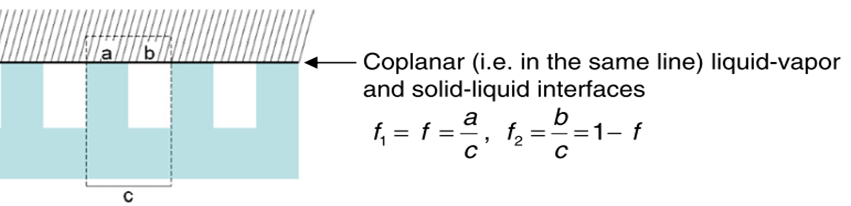
\includegraphics[width=0.7\linewidth]{cassie_coplanar}
	\caption{Schematic close up of three rough 2-D surfaces. Solid is blue/gray, air is white, liquid is the cross-hatched area above the surface. Liquid–vapor and solid–liquid interfaces of drop are denoted by the black line. A smooth-topped rough surface, which (for zero penetration of liquid) has coplanar solid–liquid and liquid–vapor interface (i.e. interfaces are in line with each other). This yields $ f_{1}=f $ and $ f_{2}=(1-f) $. Image source: \cite{Milne2012}}
	\label{fig:cassie_coplanar}
\end{figure}

Preliminary two-liquid-phase method experiments on muscovite mica showed quick and complete wetting of water on pristine mica surfaces cleaved in decane and hexadecane, contradictory to published results.\cite{Schultz1992} Clearly, more iterations of this experiment must be done to recreate this seminal paper's data, but this made me consider how a water droplet on a mirror-finished material of even greater surface energy (e.g. Fe and Fe alloys) would spread even faster than it had on a pristine mica surface. A \ca may not stabilize on a well-polished Galfenol sample even using this two-liquid-phase method, thus we must consider more options to create a measurable \ca that can extract Young's \ca. 

When mica samples were removed from the decane environment, they were wiped clean with lint-free wipes and further cleaned with acetone. When the samples were returned to the decane environment, a droplet wet the surface with an observable \ca. When this process was repeated in hexadecane, the observed \ca increased as observed in Schultz \etal This shows that even a rough surface can be measured for surface energy using the two-liquid-phase method. If this roughness is controlled by patterning the surface to a specific geometry, the same trend can be observed with the added benefit of a robust calculation of Young's contact angle by way of Equation \ref{cassie_coplanar}. 

Since Schultz published his seminal paper, his method has been used to measure very high surface energy materials ranging from ~50 mJ/m$^{2}$ to 487 mJ/m$^{2}$.\cite{Nakamura2015} However, many of these studies fail to consider the wetting modes of water on their solid surfaces in a bulk \nalk environment. Giljean \etal examines the dependence of contact angles on the roughness of high surface energy titanium surfaces using the two-liquid-phase method. They show that, depending on the cleaning technique used to remove surface contaminations, the contact angle will change more with a decrease in roughness. Sound arguments are made for the type of wetting regime (Wenzel, Cassie-Baxter, or somewhere in-between) encountered at each step of wetting. An issue occurs when the authors attempt to use the Cassie-Baxter equation to calculate the Young \ca. The Cassie-Baxter equation (Equation \ref{cassie_gen}), as defined in the original publication,\cite{Cassie1944} is designed for a general surface, where $f_1$ is the \textit{total} area of solid under the drop per unit projected area under the drop and $\theta_Y,1$ is the contact angle on a smooth surface of material 1. $f_2$ is defined similarly to $f_2$ where material 2 is air or some other medium. Many papers, as pointed out by Milne \etal,\cite{Milne2012} falsely use Equation \ref{cassie_coplanar} for randomly rough surfaces when this equation is for the special case of a coplanar liquid-vapor and solid-liquid interface, as illustrated in Figure \ref{fig:cassie_coplanar}. To use this simple equation, a surface would have to be patterned with rectangular pillars with a small enough spacing to prevent capillary forces from causing the liquid to penetrate the roughness. Keeping this in mind, I moved to the two-liquid-phase experiment originally performed on cleaved mica sheets. 
\begin{equation}
\label{cassie_gen}	
\cos\theta_{CB} = f_{1}\cos\theta_{Y} - f_{2}
\end{equation}
\begin{equation}
\label{cassie_coplanar}	
\cos\theta_{CB} = f\cos\theta_{Y} - (1-f)
\end{equation}

Considering all these factors, I postulate that by combining the two-liquid-phase method with a patterned surface of single-crystal Galfenol, the probe water droplet will not spread and a Young's \ca can be calculated for use in measuring the orientation-dependent surface energy of Galfenol. Single-crystal Galfenol samples were prepared at the DOE Ames Laboratory by the modified Bridgman technique at compositions of \fegacomp where $x=19,25$. These samples can be cut to obtain target orientations \hkl(100), \hkl(110), and \hkl(111) using electro-discharge machining. The isotropic surface created by single-crystal samples ensure that the triple-phase-line will maintain exactly the same $L_1-S$ interaction about the entire droplet perimeter. The patterned surfaces will be etched to have large enough pillars which retain as much surface orientation dependence on the contact angle as possible, as well as small enough gaps to allow for a Cassie-Baxter state in the $ L_1-L_2-S $ system. A Cassie-Baxter wetting mode would offer the greatest \ca of the three main wetting modes illustrated in Figure \ref{fig:young_cassie_wenzel}, and if a well patterned surface can be achieved similar to Figure \ref{fig:cassie_coplanar}, the Young \ca can be easily calculated from Equation \ref{cassie_coplanar}. 

Possible errors with this method will arise from non-atomically flat surfaces and pillars, imperfect Cassie-Baxter states caused by gravity or capillary forces drawing the probe liquid into the gaps between pillars, and oxide formation at the sample surface. However, such errors should be neglible given extensive polishing protocol, the immiscibility of water with \nalk[s], a controlled surface patterning, and a known cleaning procedure for rough metal surfaces. Therefore, I propose the assumption that our $ L_1-L_2-S $ system can be treated as the coplanar state depicted in Figure \ref{fig:cassie_coplanar} is reasonable. Concerning the displacement of \nalk[s] by water during the droplet depositing step, the wetting criteria has been proven by Schultz \etal\cite{Schultz1992,Giljean2011}. 

%This observable \ca is obviously a result of roughening the surface. , but because the trend of increasing \ca persists, I hypothesize that an induced roughness on isotropic metal surfaces could show increasing \ca[s] with increasing \nalk chain lengths. These induced roughnesses will be known, and using Wenzel\cite{Wenzel1936,Wenzel1949a} and Cassie\cite{Cassie1944} methods for calculating equilibrium \ca[s] and, resultantly, the orientation-dependent Galfenol surface energy. 
%TODO: CONTINUE HERE PLEASE. INSERT ASSUMPTIONS TO BE MADE AND THEN EXTEND TO ORIENTATION DEPENDENCE ON GALFENOL SINGLE CRYSTALS.

%\begin{figure}[h]
%	\centering
%	\begin{subfigure}[c]{0.47\textwidth}
%		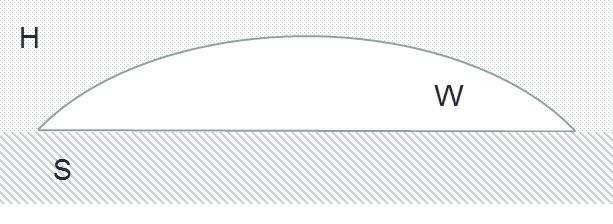
\includegraphics[width=\linewidth]{ideal-flat-two-liq}
%		\subcaption{~}
%		\label{fig:ideal-flat-two-liq}		
%	\end{subfigure}
%	\begin{subfigure}[c]{0.47\textwidth} 
%		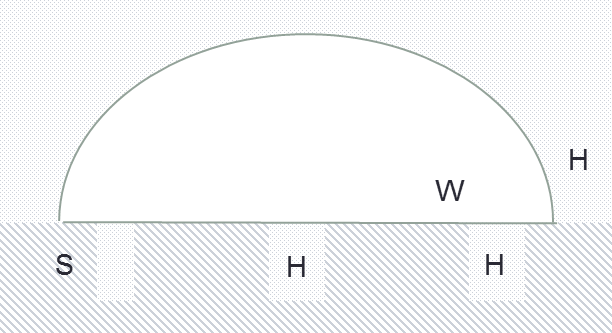
\includegraphics[width=\linewidth]{cassie-two-liq}
%		\subcaption{~}
%		\label{fig:cassie-two-liq}		
%	\end{subfigure}
%	\caption{(a) Ideally flat two-liquid-phase method (b) Cassie mode two-liquid-phase method }
%	\label{fig:goss_se_msrmnt}
%\end{figure}

\begin{figure}[h]
	\centering
	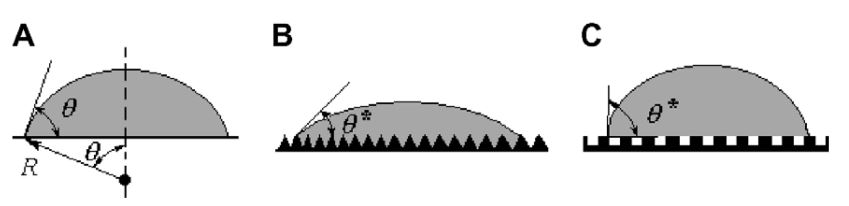
\includegraphics[width=\linewidth]{young_cassie_wenzel}
	\caption{Schemes of different wetting regimes. A – flat substrate; B – rough substrate, the Wenzel regime; C – rough substrate with air trapped under the drop, the Cassie–Baxter regime.\cite{Whyman2008}}
	\label{fig:young_cassie_wenzel}
\end{figure}

%The procedure for carrying out this study is as follows:
\subsubsection{Experimental plan}
%\renewcommand{\outlineii}{cenumerate}
%\begin{outline}[enumerate]
%\setlength{\itemindent}{0em}
\textbf{1)} For measuring the dispersive solid surface energy component, four different acrylic glass (Poly(methyl methacrylate), PMMA) boxes for hexane, octane, decane, and hexadecane environments will be used to contain the experiment. Acrylic has a high chemical compatibility with \nalk[s], and the transparent optical properties will not affect the contact angle pictures taken.\cite{Thermoscientific} Since most adhesives are stored in \nalk[s] (also commonly used as industrial strength degreasers), PMMA boxes must be chemically welded together by a solvent at room temperature to keep the liquid environment contained. The same boxes will be created for the other liquid mediums used to measure the polar solid surface energy component. \\
\textbf{2)} Single-crystal samples (\fegacomp where $x=19,25$) will be polished using SiC paper followed by 0.1 $\mu$m particle colloidal silica gel to achieve a mirror finish. EBSD or single-crystal XRD is used to find surface orientation. After the main sample surface orientation is discovered, the sample can be cut using wire cut electric discharge machining to obtain \hkl(001), \hkl(110), and \hkl(111) facets. Each sample is then polished again for EBSD measurement and surface energy measurement. As soon as polished samples have reached a mirror-finish, they will be immersed in the \nalk environment. \\ 
\textbf{3)} Samples will be mounted with the surface perpendicular to the dispensing needle and the two-liquid-phase method will be administered. This first experiment will attempt to measure a \ca on the polished Galfenol samples, but the probe water will likely spread over the surface very quickly to achieve complete wetting. Advancing and receding \ca[s] will be measured to find the contact angle hysteresis (CAH), as well as the drop volume of respective angles.  A group from the Max Planck Institute for Polymer Research has recently observed microscopic videos of water CAH on pillared polymer surfaces using laser scanning confocal microscopy.\cite{Butt2016,Schaffel2016} The UMD Department of Cell Biology and Molecular Genetics has two confocal microscopes that will be utilized to accurately measure the CAH of every Galfenol sample. By comparing this result to the CAH measured using the telescopic goniometer, we determine the necessity of confocal microscopy in future measurements. Another option for recording CAH is a high speed camera that to capture the wetting line spreading and receding. Coupled with the telescopic lens on the Kruss goniometer provided by UMD's Civil \& Environmental Engineering we can use a high speed CCD camera to capture such images. From the advancing and receding \ca[s], a proper averaging can be used to estimate the most stable contact angle, as seen in Equation \ref{avg_cah}.\cite{Andrieu1994} The most stable contact angle has also been measured by simply vibrating the system for ~15 s.\cite{Meiron2004} An averaging of advancing and receding \ca[s] is reasonable considering the practical advancing and receding \ca[s] are metastable states on opposite sides of a Gibbs energy vs. contact angle plot, seen in Figure \ref{fig:gibbs_ca}.
\begin{equation}
	\label{avg_cah}	
	\cos\theta_{ms} = (\cos\theta_{a} + \cos\theta_{r})/2 
\end{equation}
\begin{wrapfigure}[16]{r}{0.45\linewidth}
	\centering
	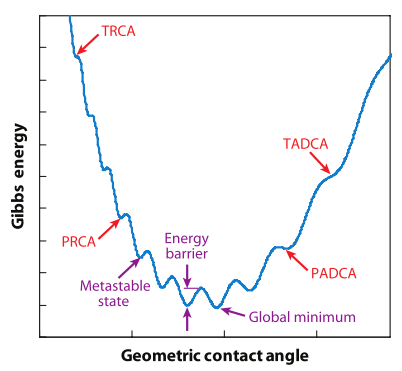
\includegraphics[width=\linewidth,trim={0 0 0 1cm}]{gibbs_ca}
	\caption{The curve of Gibbs energy versus geometric contact angle for a two-dimensional drop on a heterogeneous solid surface. Each minimum represents a metastable equilibrium state. The lowest of all minima indicates the most stable state. In between every pair of equilibrium states there exists an energy barrier. Abbreviations used: PADCA, practical advancing contact angle; PRCA, practical receding contact angle; TADCA, theoretical advancing contact angle; TRCA, theoretical receding contact angle.\cite{Marmur2009b}}
	\label{fig:gibbs_ca}
\end{wrapfigure}
The drop volumes of advancing and receding \ca[s] will give us a range of volumes for static \ca measurements on the same surfaces, which are also expected to totally wet our flat surfaces, but will be measured to validate that assumption.\\
\textbf{4)} I will  work with UMD's FabLab to determine the best protocol for creating a patterned surface on Fe-Ga samples. Patterning will occur on the mirror-finish samples made in Step 2 to ensure the flattest possible pillars. With well patterned surfaces, I will execute the same two-liquid-phase method procedure described in Step 3. I expect much greater contact angles for every surface based on the controlled roughness, and I also expect dramatic differences in the calculated solid surface energies for the \hkl(100), \hkl(110), and \hkl(111) Fe-Ga surfaces using Equation \ref{gamS}. \\
\textbf{5)} These surface energy values should be similar to the $\alpha$-iron DFT calculations of $\gamma_{100}$ = 2.6660 J/m$^2$, $\gamma_{110}$ = 2.0535 J/m$^2$, and $\gamma_{111}$ = 2.5271 J/m$^2$.\cite{Wang2000} While testing single-crystal samples of two different compositions (\fegacomp where $x=19,25$), it is unclear how the surface energy of Fe-Ga will change with composition. I have asked our collaborator, Dr. Ruqian Wu, to use computer simulations to try and find such a change in surface energy with composition, which I will compare with upon experimentally determining these values. 
%Pattern surfaces with transparency paper $\gtrsim$40 $\mu$m since this is the lower limit of transparency paper. 



%	\2 The assumption of this patterned surface is that the Cassie-Baxter or Wenzel contact angle is the most stable contact angle, and the Young contact angle can be approximated using the Cassie-Baxter and Wenzel equations. This contact angle will be suitable for the of metal surface energy that will be calculated from Equation \ref{schultz2}.
%		\3 There seems to be controversy in literature on whether the equilibrium contact angle calculated in Cassie and Wenzel equations can be used as the Young \ca.\cite{Attension2015,Marmur2009b,Bracco2013}
%		\3 The Cassie-Baxter contact angle is an equilibrium contact angle as proven by Johnson and Dettre using thermodynamic principles.\cite{Johnson1964}
%		\3 The most stable contact angle on a rough surface is either the Wenzel or Cassie angle, IF the size of the drop is two to three orders of magnitude larger than the typical scale of roughness.\cite{Meiron2004} %TODO: read the paper cited, about sufficient drop size vs. roughness
%	\2 Preliminary two-liquid-phase method experiments on muscovite mica showed quick and complete wetting of water on pristine mica surfaces cleaved in decane and hexadecane, contradictory to published results.\cite{Schultz1992} When mica samples were removed from the decane environment, they were wiped clean with KimWipes and further cleaned with acetone. When the samples were returned to the decane environment, a droplet wet the surface with an observable \ca. When this process was repeated in hexadecane, the observed \ca increased as observed in Schultz et al.\cite{Schultz1992} 
%	
%	This observable \ca is a result of roughening the surface, but because the trend of increasing \ca persists, I hypothesize that an induced roughness on isotropic metal surfaces could show increasing \ca[s] with increasing \nalk chain lengths. These induced roughnesses will be known, and using Wenzel\cite{Wenzel1936,Wenzel1949a} and Cassie\cite{Cassie1944} methods for calculating equilibrium \ca[s] and, resultantly, the orientation-dependent Galfenol surface energy. 
%		
%	\2 Per conversation with Dave Shahin, an experienced student in patterning surfaces, an array of roughnesses can be made on a single sample to test roughness effects on surface energy measurements of single crystal Galfenol and Alfenol. 
%		\3 There is a criteria for determining if the calculated contact angle on a rough surface is in Wenzel and Cassie-Baxter modes.\cite[p. 53]{Milne2012}
%	
%\1 Redo two-liquid-phase experiment for patterned surface
%	\2 Calculate the Cassie and Wenzel mode equilibrium CA
%		\3 Expecting Cassie mode because the patterned channels will ideally be completely filled with hydrocarbon/\nalk liquid, thus \underline{repelling} the water droplet on the surface. This is due to the immiscibility of polar (distilled water) and non-polar (\nalk) solvents. 
%	\2 \textbf{Is there a difference from one patterned orientation to another?} This will show if the patterning (induced roughness) will have a large impact on the CA and, as a result, \underline{Surface Energy}. 
%		\3 If we have a defined roughness for {100}, {110}, and {111} samples, and the apparent \ca[s] do not change with orientation, the geometry of the roughness dictates the \ca. 
%		\3 If the \ca[s] do change with orientation, the surface orientation determines the \ca, and surface energy can be confidently measured.
%\end{outline}

Pending the success of this proposed research, our group will incorporate these experimentally determined orientation-dependent surface energies into to our AGG model to elucidate the driving forces of grain growth methods in Galfenol. We would like to expand this experiment to single-crystal Alfenol samples as well as many other pure and alloyed metals. Metal surface energies are extremely elusive values due to their complexities and lack of consistent experimental confirmation. My goal is that this work will contribute to the vast body of work on experimental wetting dynamics and surface energy determination for the benefit research in the near future and push the boundaries of understanding.


%\subsection{Timeline}
%What follows in Table [  ] is a projected timeline for completion of the proposed research, leading to a defense and graduation in the Winter of 2017. 
%
%\begin{table}[h]
%	\renewcommand\arraystretch{1.4}%\arrayrulecolor{LightSteelBlue3}
%	\captionsetup{singlelinecheck=false, labelfont=sc, labelsep=quad}
%	\caption{Timeline of proposed research}\vskip -1.5ex
%	\begin{tabular}{@{\,}r <{\hskip 2pt} !{\foo} >{\raggedright\arraybackslash}p{13.7cm}}
%		\toprule
%%		\addlinespace[1.5ex]
%		June 2016 & AT and T Bell Labs develop the idea of cellular phones\\
%		July 2016 & Xerox Palo Alto Research Centre envisage the 'Dynabook\\
%		Aug 2016 & Busicom 'Handy-LE' Calculator\\
%		Sept 2016 & First mobile handset invented by Martin Cooper\\
%		Oct 2016 & Parker Bros. Merlin Computer Toy\\
%		Nov 2016 & Osborne 1 Portable Computer\\
%		Dec 2016 & Grid Compass 1100 Clamshell Laptop\\
%		Jan 2017 & TRS-80 Model 100 Portable PC\\
%	\end{tabular}
%\end{table}

%\subsection{Induced roughness for Wenzel and Cassie modes}

%\subsection{DFT measurements from collaborator}
%\subsubsection{Cassie-Baxter or Wenzel mode}
%\textbf{Can Dr. Ruqian Wu simulate a sessile drop in a two-liquid-phase experiment on a patterned surface?} This can tell us if we can expect Cassie of Wenzel mode of water drop in hydrocarbon/\nalk environment. 
%
%\subsubsection{Two compositions of single crystal Galfenol}
%Dr. Wu has assigned a student to working on a difference in \fegacomp surface energy where $x =$ 19 and 25.

\chapter{Conclusion}
In conclusion...

\newpage
\appendix
\chapter{Derivation of Young's Equation}\label{appendixA}


Assuming an ideally flat surface
\begin{equation} \label{dropvol}
V_{drop} = \frac{\pi R^{3}}{3} (1-\cos\theta)^{2} (2+\cos\theta)
\end{equation}
\begin{equation} \label{liqvapSA}
S_{LV} = 2\pi R^{2} (1-\cos\theta)
\end{equation}

Where $S_{LV}$ is the surface area of the droplet liquid-vapor interface. The Gibbs free energy of a droplet is depicted in Equation \ref{gibbsdroplet}.

\begin{equation} \label{gibbsdroplet}
G = \gamma_{LV} S_{LV} + \pi(R \sin\theta)^{2} \underbracket{(\gamma_{SL}-\gamma_{SV})}_{\text{\normalsize{$a$}}}\\
\end{equation}

where \gamLV, \gamSL, and \gamSV are the liquid-vapor, solid-liquid, and solid-vapor interaction energies, respectively. Let $a = \gamma_{SL}-\gamma_{SV}$. 

Assuming the the volume of the droplet remains constant:
\begin{equation*}
	\begin{gathered}
		G = \left[\frac{9\pi V^{2}}{(1-\cos\theta)(2+\cos\theta)^{2}}\right]^{2/3}
		\left[2\gamma_{LV} - a(1+\cos\theta)\right]\\
		\frac{dG}{d\theta} = \left[\frac{9\pi V^{2}}{(1-\cos\theta)^{4}(2+\cos\theta)^{5}}\right]^{1/3}
		2\left[a-\gamma_{LV}\cos\theta)\right]\sin\theta\\ \\
		\begin{split}
			\left[\frac{dG}{d\theta}\right]_{\theta=\theta_{eq}}&=0=a-\gamma_{LV}\cos\theta\\
			\therefore a 	&= \gamma_{LV}\cos\theta\\
		\end{split}					
	\end{gathered}
\end{equation*}

\chapter{Derivation of Schultz's two-liquid-phase method}\label{appendixB}
\subsection{Measuring dispersive solid surface energy, $\gamma_{S}^{D}$}
	
Assuming Young's equation (Equation \ref{young_eqn}) can be applied to a liquid-liquid(bulk phase)-solid ($L_{1}-L_{2}-S$) system, and the relationship follows:
\begin{equation}
\label{youngs}
	\gamma_{SL_{2}} = \gamma_{L_{1}L_{2}}\cos\theta_{SL_{1}} + \gamma_{SL_{1}}
\end{equation}

In this way, \gamSV, which is the driving force of spreading the one-liquid-phase method that causes complete wetting on high-surface energy metal surfaces, is replaced by $ \gamma_{SL_{2}} $, where $\gamma_{SL_{2}} <$ \gamSV. Hence, the contact angle in this system is measurable. According to Fowkes\cite{Fowkes1964}, $\gamma_{SL_{1}}$ and $\gamma_{SL_{2}}$ are given by:
\begin{equation} 
\label{gSL1}
	\gamma_{SL_{1}} = \gamma_{S} + \gamma_{L_{1}} - 2(\gamma_{S}^{D}\gamma_{L_{1}}^{D}) - I_{SL_{1}}^{P}
\end{equation}
\begin{equation}
\label{gSL2}
	\gamma_{SL_{2}} = \gamma_{S} + \gamma_{L_{2}} - 2(\gamma_{S}^{D}\gamma_{L_{2}}^{D}) - I_{SL_{2}}^{P}
\end{equation} 
where $\gamma$ and $\gamma^{D}$ are the surface energy and its dispersive component, respectively, and $I_{SL_{1}}^{P}$ is a specific (nondispersive) interaction term that encompasses all interactions between the solid and the liquid (dipole-dipole, dipole-induced dipole, hydrogen bonds, $\pi$ bonds, etc.) except London dispersion interactions.

%TODO Define and understand dispersive vs. polar components of surface energy.
%TODO Define and understand London dispersion forces
Substituting Equations \ref{gSL1} and \ref{gSL2} into \ref{youngs}:

\begin{equation} 
\label{schultz1}
	\gamma_{SL_{1}}-\gamma_{SL_{2}}+\gamma_{L_{1}L_{2}}\cos\theta_{SL_{1}} = 2(\gamma_{S}^{D})^{1/2}  [(\gamma_{L_{1}}^{D})^{1/2}-(\gamma_{L_{2}}^{D})^{1/2}] + I_{SL_{1}}^{P} - I_{SL_{2}}^{P}
\end{equation}

$L_{1}$ will signify water, $L_{2}$ as \nalk[s], and $I_{SL_{2}}^{P}$ may be considered equal to zero because the surface free energy of \nalk[s] only consists of the London dispersion term. This is because \nalk[s] only contain C-C and C-H atoms connected by $\sigma$-bonds, with a generic formula of C$_{n}$H$_{2n+2}$. C and H have very similar electronegativities of $\chi_{C}=2.55$ and $\chi_{H}=2.20$, respectively. This shows that all bonds in \nalk[s] are non-polar, hence there are no polar interactions in \nalk[s]. Our final equation is now:

\begin{equation} 
\label{schultz2}
	\gamma_{W}-\gamma_{H}+\gamma_{WH}\cos\theta_{W} = 2(\gamma_{S}^{D})^{1/2}[(\gamma_{W}^{D})^{1/2}-(\gamma_{H}^{D})^{1/2}] + I_{SW}^{P} 
\end{equation} 

In order to calculate the dispersive component of \gamSV for a solid surface, the water \ca must be measured on a solid immersed in \nalk[s]. By interpreting Equation \ref{schultz2} as a classic linear function, $y = mx + b$:

\[
\underbracket{\gamma_{W}-\gamma_{H}+\gamma_{WH}\cos\theta_{W}}_{\text{\normalsize{$y$}}} =
\underbracket{2(\gamma_{S}^{D})^{1/2}}_{\text{\normalsize{$m$}}}  
\underbracket{[(\gamma_{W}^{D})^{1/2}-(\gamma_{H}^{D})^{1/2}] }_{\text{\normalsize{$x$}}} + 
\underbracket{I_{SW}^{P}}_{\text{\normalsize{$b$}}} 
\] 

\subsection{Measuring polar solid surface energy, $\gamma_{S}^{P}$}

Beginning with Equation \ref{schultz1} in the previous section and solving for $ I_{SL_{2}}^{P} $, with liquid $L_1$ as water (subscript $ W $):

\begin{equation}
	I_{L_2}^{P} = \gamma_{SL_2}-\gamma_{WL_2}\cos\theta_{SW}-2(\gamma_{S}^{D}\gamma_{L_2}^{D})^{1/2} + C
\end{equation}
\begin{equation}
	C = I_{SW}^{P} + 2(\gamma_{S}^{D}\gamma_{W}^{D})^{1/2} - \gamma_W
\end{equation}

In the above two equations, the values of $ \gamma_W$, $ \gamma_{W}^{D} $, $ \gamma_{S}^{D} $, and $I_{SW}^{P}$ are available experimentally from the previous section. Therefore, measurements of $ \gamma_{L_2}$, $ \gamma_{L_2}^{D} $, $\theta_{SW}$, and $ \gamma_{L_2}^{D} $ lead to a calculation of the polar interaction $I_{SL_{2}}^{P}$. 

For calculating the polar interaction between a solid and a liquid from the polar term of their surface free energy, a geometric-mean relation is used, shown in Equation \ref{polarinteractionline}. 
\begin{equation} \label{polarinteractionline}
	I_{SL_{2}}^{P} = 2(\gamma_{S}^{P}\gamma_{L_{2}}^{P})^{1/2}
\end{equation}

We find $ \gamma_{S}^{P} $ by plotting values of $ I_{SL_{2}}^{P} $ vs. $\sqrt{ \gamma_{L_{2}}^{P} }$ for a set of chloroalkane and nitroalkane bulk liquids with a polar component of surface tension.

\[
\underbracket{ I_{SL_{2}}^{P}}_{\textbf{\normalsize{$y$}} } =
\underbracket{ 2\sqrt{\gamma_{S}^{P} }} _{\textbf{\normalsize{$m$}} }
\underbracket{ \sqrt{\gamma_{L_{2}}^{P} }} _{\textbf{\normalsize{$x$}}  }
\]





\newpage
\bibliographystyle{unsrt}
\bibliography{Bibtex/library}


\end{document}